\documentclass[aspectratio=169,compress]{beamer}

\usepackage{biblatex}
\bibliography{citation.bib}

\usepackage{fontawesome}
\usepackage[english]{babel}
\usepackage{metalogo}
\usepackage{listings}
\usepackage{fontspec}
\usepackage{tikz}

\usepackage{caption}
\usepackage{subcaption}

\lstdefinelanguage
   {SASS}     % add a "x64" dialect of Assembler
   [x86masm]{Assembler} % based on the "x86masm" dialect
   % with these extra keywords:
   {morekeywords={LDS,STS,ISETP.EQ.AND,MOV32I,STG.E,IADD,LDG.E,ISETP.NE.AND,BRA,LDG.E.STRONG.SYS,
                  IMAD.MOV.U32,STG.E.STRONG.SYS}}

\usetikzlibrary{calc}
\usetikzlibrary{shapes.geometric}
\usepackage{etoolbox}

\pgfdeclarelayer{background}
\pgfdeclarelayer{foreground}
\pgfdeclarelayer{sankeydebug}
\pgfsetlayers{background,main,foreground,sankeydebug}

\newif\ifsankeydebug

\newenvironment{sankeydiagram}[1][]{

  \def\sankeyflow##1##2{% sn, en
    \path[sankey fill]
    let
    \p1=(##1.north east),\p2=(##1.south east),
    \n1={atan2(\y1-\y2,\x1-\x2)-90},
    \p3=(##2.north west),\p4=(##2.south west),
    \n2={atan2(\y3-\y4,\x3-\x4)+90}
    in
    (\p1) to[out=\n1,in=\n2] (\p3) --
    (\p4) to[in=\n1,out=\n2] (\p2) -- cycle;
    \draw[sankey draw]
    let
    \p1=(##1.north east),\p2=(##1.south east),
    \n1={atan2(\y1-\y2,\x1-\x2)-90},
    \p3=(##2.north west),\p4=(##2.south west),
    \n2={atan2(\y3-\y4,\x3-\x4)+90}
    in
    (\p1) to[out=\n1,in=\n2] (\p3)
    (\p4) to[in=\n1,out=\n2] (\p2);
  }


  \tikzset{
    sankey tot length/.store in=\sankeytotallen,
    sankey tot quantity/.store in=\sankeytotalqty,
    sankey min radius/.store in=\sankeyminradius,
    sankey arrow length/.store in=\sankeyarrowlen,
    sankey debug/.is if=sankeydebug,
    sankey debug=false,
    sankey flow/.style={
      to path={
        \pgfextra{
          \pgfinterruptpath
          \edef\sankeystart{\tikztostart}
          \edef\sankeytarget{\tikztotarget}
          \sankeyflow{\sankeystart}{\sankeytarget}
          \endpgfinterruptpath
        }
      },
    },
    sankey node/.style={
      inner sep=0,minimum height={sankeyqtytolen(##1)},
      minimum width=0,draw=none,line width=0pt,
    },
    % sankey angle
    sankey angle/.store in=\sankeyangle,
    % sankey default styles
    sankey fill/.style={line width=0pt,fill,white},
    sankey draw/.style={draw=black,line width=.4pt},
  }

  \newcommand\sankeynode[4]{%prop,orientation,name,pos
    \node[sankey node=##1,rotate=##2] (##3) at (##4) {};
  }

  \newcommand\sankeynodestart[4]{%prop,orientation,name,pos
    \sankeynode{##1}{##2}{##3}{##4}
    \begin{scope}[shift={(##3)},rotate=##2]
      \path[sankey fill]
      (##3.north west) -- ++(-\sankeyarrowlen,0)
      -- ([xshift=-\sankeyarrowlen/6]##3.west)
      -- ([xshift=-\sankeyarrowlen]##3.south west)
      -- (##3.south west) -- cycle;
      \path[sankey draw]
      (##3.north west) -- ++(-\sankeyarrowlen,0)
      -- ([xshift=-\sankeyarrowlen/6]##3.west)
      -- ([xshift=-\sankeyarrowlen]##3.south west)
      -- (##3.south west);
    \end{scope}
  }

  \newcommand\sankeynodeend[4]{%prop,orientation,name,pos
    \sankeynode{##1}{##2}{##3}{##4}
    \begin{scope}[shift={(##3)},rotate=##2]
      \path[sankey fill]
      (##3.north east)
      -- ([xshift=\sankeyarrowlen]##3.east)
      -- (##3.south west) -- cycle;
      \path[sankey draw]
      (##3.north east)
      -- ([xshift=\sankeyarrowlen]##3.east)
      -- (##3.south west);
    \end{scope}
  }

  \newcommand\sankeyadvance[3][]{%newname,name,distance
    \edef\name{##2}
    \ifstrempty{##1}{
      \def\newname{##2}
      \edef\name{##2-old}
      \path [late options={name=##2,alias=\name}];
    }{
      \def\newname{##1}
    }
    \path
    let
    % sankey node angle
    \p1=(##2.north east),
    \p2=(##2.south east),
    \n1={atan2(\y1-\y2,\x1-\x2)-90},
    % sankey prop
    \p3=($(\p1)-(\p2)$),
    \n2={sankeylentoqty(veclen(\x3,\y3))},
    % next position
    \p4=($(##2.east)!##3!-90:(##2.north east)$)
    in
    \pgfextra{
      \pgfmathsetmacro{\prop}{\n2}
      \pgfinterruptpath
      \sankeynode{\prop}{\n1}{\newname}{\p4}
      \path (\name) to[sankey flow] (\newname);
      \endpgfinterruptpath
    };
  }

  \newcommand\sankeyturn[3][]{%newname,name,angle
    \edef\name{##2}
    \ifstrempty{##1}{
      \def\newname{##2}
      \edef\name{##2-old}
      \path [late options={name=##2,alias=\name}];
    }{
      \def\newname{##1}
    }
    \ifnumgreater{##3}{0}{
      \typeout{turn acw: ##3}
      \path
      let
      % sankey node angle
      \p1=(##2.north east),
      \p2=(##2.south east),
      \p3=($(\p1)!-\sankeyminradius!(\p2)$),
      \n1={atan2(\y1-\y2,\x1-\x2)-90},
      % sankey prop
      \p4=($(\p1)-(\p2)$),
      \n2={sankeylentoqty(veclen(\x4,\y4))},
      \p5=(##2.east),
      \p6=($(\p3)!1!##3:(\p5)$)
      in
      \pgfextra{
        \pgfmathsetmacro{\prop}{\n2}
        \pgfinterruptpath
        % \fill[red] (\p3) circle (2pt);
        % \fill[blue](\p6) circle (2pt);
        \sankeynode{\prop}{\n1+##3}{\newname}{\p6}
        \path (\name) to[sankey flow] (\newname);
        \endpgfinterruptpath
      };
    }{
      \typeout{turn acw: ##3}
      \path
      let
      % sankey node angle
      \p1=(##2.south east),
      \p2=(##2.north east),
      \p3=($(\p1)!-\sankeyminradius!(\p2)$),
      \n1={atan2(\y1-\y2,\x1-\x2)+90},
      % sankey prop
      \p4=($(\p1)-(\p2)$),
      \n2={sankeylentoqty(veclen(\x4,\y4))},
      \p5=(##2.east),
      \p6=($(\p3)!1!##3:(\p5)$)
      in
      \pgfextra{
        \pgfmathsetmacro{\prop}{\n2}
        \pgfinterruptpath
        % \fill[red] (\p3) circle (2pt);
        % \fill[blue](\p6) circle (2pt);
        \sankeynode{\prop}{\n1+##3}{\newname}{\p6}
        \path (\name) to[sankey flow] (\newname);
        \endpgfinterruptpath
      };
    }
  }

  \newcommand\sankeyfork[2]{%name,list of forks
    \def\name{##1}
    \def\listofforks{##2}
    \xdef\sankeytot{0}
    \path 
    let
    % sankey node angle
    \p1=(\name.north east),
    \p2=(\name.south east),
    \n1={atan2(\y1-\y2,\x1-\x2)-90},
    % sankey prop
    \p4=($(\p1)-(\p2)$),
    \n2={sankeylentoqty(veclen(\x4,\y4))}
    in
    \pgfextra{
      \pgfmathsetmacro{\iprop}{\n2}
    }
    \foreach \prop/\name[count=\c] in \listofforks {
      let
      \p{start \name}=($(\p1)!\sankeytot/\iprop!(\p2)$),
      \n{nexttot}={\sankeytot+\prop},
      \p{end \name}=($(\p1)!\n{nexttot}/\iprop!(\p2)$),
      \p{mid \name}=($(\p{start \name})!.5!(\p{end \name})$)
      in
      \pgfextra{
        \xdef\sankeytot{\n{nexttot}}
        \pgfinterruptpath
        \sankeynode{\prop}{\n1}{\name}{\p{mid \name}}
        \endpgfinterruptpath
      }
    }
    \pgfextra{
      \pgfmathsetmacro{\diff}{abs(\iprop-\sankeytot)}
      \pgfmathtruncatemacro{\finish}{\diff<0.01?1:0}
      \ifnumequal{\finish}{1}{}{
        \message{*** Warning: bad sankey fork (maybe)...}
        \message{\iprop-\sankeytot}
      }
    };
  }

  \tikzset{
    % default values,
    declare function={
      sankeyqtytolen(\qty)=\qty/\sankeytotalqty*\sankeytotallen;
      sankeylentoqty(\len)=\len/\sankeytotallen*\sankeytotalqty;
    },
    sankey tot length=100pt,
    sankey tot quantity=100,
    sankey min radius=30pt,%
    sankey arrow length=10pt,%
    % user values
    #1}
}{
}


\usetheme{Nord}
% \usetheme[style=light]{Nord}

\setmainfont{Yanone Kaffeesatz}
\setsansfont{Andika New Basic}
\setmonofont{DejaVu Sans Mono}

\title{CUDA Memory Model}
\subtitle{Or how ``our strength grows out of our weakness''}
\author{Georgy Evtushenko \faTwitter @g\_evtushenko}
\date{\today}

\lstset{language=C++,
			  numbers=left,
    		stepnumber=1,
        basicstyle=\ttfamily\small,
			  numberstyle=\color{NordBrightBlack}\ttfamily\small,
        keywordstyle=\color{NordYellow}\ttfamily\small,
        commentstyle=\color{NordGreen}\ttfamily\small,
        morecomment=[l][\color{NordGreen}]{\#},
        emph={
           __global__, __shared__, __device__, __host__, __syncthreads,
        },
        emphstyle={\color{NordBlue}},
}

\begin{document}

\begin{frame}[plain,noframenumbering]
  \maketitle
\end{frame}

\begin{frame}{Motivation}
  \begin{description}[Performance]
  \item[Performance]
		A significant slowdown is caused by excess memory ordering
  \item[Correctness]
		One source of non-deterministic concurrency bugs is a misunderstanding of the architecture’s shared 
		memory consistency model i.e. what values can be read from shared memory when issued concurrently 
		with other reads and writes. \footfullcite{PrimerOnMemoryConsistency}
  \end{description}
\end{frame}

\begin{frame}{Definitions}
  \begin{description}[Memory operation]
  \item[Read operation]
    All variants of \textcolor{NordYellow}{ld} instruction and \textcolor{NordYellow}{atom} instruction.
  \item[Write operation]
    All variants of \textcolor{NordYellow}{st} instruction and \textcolor{NordYellow}{atom} instruction.
  \item[Memory operation]
    A \textcolor{NordYellow}{read} or \textcolor{NordYellow}{write} operation.
  \item[Memory model]
    Set of rules defining how \textcolor{NordYellow}{memory operations} on shared memory from multiple threads are processed.
    Tradeoff between ease of programmability and efficiency.
  \item[Memory order]
    Total order of \textcolor{NordYellow}{memory operations}.
  \end{description}
\end{frame}

\begin{frame}[fragile]{Sequential consistency}{}
  ``... the result of any execution is the same as if the operations of all the processors were executed in some 
  sequential order, and the operations of each individual processor appear in this sequence in the order 
  specified by its program.'' \footfullcite{Lamport1979HowTM}

	\begin{columns}
			\begin{column}{0.2\textwidth}
\begin{lstlisting}[title={Thread 1}]
x = 1
r1 = y
\end{lstlisting}
			\end{column}
			\begin{column}{0.2\textwidth}
\begin{lstlisting}[title={Thread 2}]
y = 1
r2 = x
\end{lstlisting}
			\end{column}
	\end{columns}

\end{frame}

\begin{frame}{Sequential consistency}{Memory order}
	\centering
	$A \mathbin{\color{NordYellow}\mathord{<}p} B \Rightarrow A \mathbin{\color{NordYellow}\mathord{<}m} B$
	\begin{columns}[T]
		\begin{column}{0.34\textwidth}
			\begin{figure}
				\centering
				\resizebox{1.1\textwidth}{!}{%
				\begin{tikzpicture}
					\begin{sankeydiagram}[
						sankey tot length=30pt,%
						sankey tot quantity=6,%
						sankey min radius=15pt,%
						sankey fill/.style={
							draw,line width=0pt,
							fill,
							NordGreen,
						},
						sankey draw/.style={
							draw=white, %NordBlack,
							line width=1pt,
							line cap=round,
							line join=round,
						},
						%	sankey debug,
						]

						% First thread
						\sankeynode{6}{0}{t0i0}{0,0};
						\sankeyadvance{t0i0}{60pt}

						\sankeyfork{t0i0}{3/p1,3/p2}

						% \sankeyturn{p1}{20}
						% \sankeyadvance{p2}{20pt}

						\sankeynode{6}{0}{p11}{[shift={(15pt,15pt)}]t0i0}
						\sankeyfork{p11}{3/p11a,3/p12a}
						\path (p1) to[sankey flow] (p11a);
						\path (p2) to[sankey flow] (p12a);

						\node[anchor=west,text=NordDarkBlack] at (0,0.25) {x = 1};
						\node[anchor=west,text=NordDarkBlack] at (0,-0.25) {r1 = y};

						\node[anchor=east] (p11as) at (p11a) {};
						\node[anchor=east] (p12as) at (p12a) {};

						\sankeyadvance{p11a}{55pt}
						\sankeyadvance{p12a}{55pt}

						\node[anchor=west,text=NordDarkBlack] at ([shift={(8pt,0pt)}]p11as) {store x};
						\node[anchor=west,text=NordDarkBlack] at ([shift={(8pt,0pt)}]p12as) {load y};


					% Second thread
					{
						\tikzset{
							sankey fill/.append style={
								draw,line width=0pt,
								fill,
								NordBlue,
							}
						}
						\sankeynode{6}{180}{t1i0}{[shift={(142pt,0pt)}]t0i0};
						\sankeyadvance{t1i0}{57pt}
						\sankeyfork{t1i0}{3/p3,3/p4}

						\sankeynode{6}{180}{p14}{[shift={(70pt,-15pt)}]t0i0}
						\sankeyfork{p14}{3/p14a,3/p15a}
						\path (p3) to[sankey flow] (p14a);
						\path (p4) to[sankey flow] (p15a);
						\sankeyadvance{p14a}{55pt}
						\sankeyadvance{p15a}{55pt}

						\node[anchor=west,text=NordDarkBlack] at ([shift={(4pt,0pt)}]p14a) {load x};
						\node[anchor=west,text=NordDarkBlack] at ([shift={(4pt,0pt)}]p15a) {store y};

						\node[anchor=west,text=NordDarkBlack] at (145pt,0.25) {y = 1};
						\node[anchor=west,text=NordDarkBlack] at (145pt,-0.25) {r2 = x};
					}

						\draw [densely dashed,thick,draw=NordWhite] (0pt,30pt) -- (0pt,-65pt);
						\draw [densely dashed,thick,draw=NordWhite] (75pt,30pt) -- (75pt,-65pt);
						\draw [densely dashed,thick,draw=NordWhite] (130pt,30pt) -- (130pt,-65pt);
						\draw [densely dashed,thick,draw=NordWhite] (202pt,30pt) -- (202pt,-65pt);

					\begin{scope}[shift={(0pt,-80pt)}]
						sankey tot length=30pt,%
						sankey tot quantity=6,%
						sankey min radius=15pt,%
						sankey fill/.style={
							draw,line width=0pt,
							fill,
							NordGreen,
						},
						sankey draw/.style={
							draw=white, %NordBlack,
							line width=1pt,
							line cap=round,
							line join=round,
						},
						%	sankey debug,
						]

						% First thread
						\sankeynode{6}{0}{t0i0}{0,0};
						\sankeyadvance{t0i0}{60pt}

						\sankeyfork{t0i0}{3/p1,3/p2}

						% \sankeyturn{p1}{20}
						% \sankeyadvance{p2}{20pt}

						\sankeynode{6}{0}{p11}{[shift={(15pt,-15pt)}]t0i0}
						\sankeyfork{p11}{3/p11a,3/p12a}
						\path (p1) to[sankey flow] (p11a);
						\path (p2) to[sankey flow] (p12a);

						\node[anchor=west,text=NordDarkBlack] at (0,0.25) {x = 1};
						\node[anchor=west,text=NordDarkBlack] at (0,-0.25) {r1 = y};

						\node[anchor=east] (p11as) at (p11a) {};
						\node[anchor=east] (p12as) at (p12a) {};

						\sankeyadvance{p11a}{55pt}
						\sankeyadvance{p12a}{55pt}

						\node[anchor=west,text=NordDarkBlack] at ([shift={(8pt,0pt)}]p11as) {store x};
						\node[anchor=west,text=NordDarkBlack] at ([shift={(8pt,0pt)}]p12as) {load y};


					% Second thread
					{
						\tikzset{
							sankey fill/.append style={
								draw,line width=0pt,
								fill,
								NordBlue,
							}
						}
						\sankeynode{6}{180}{t1i0}{[shift={(142pt,0pt)}]t0i0};
						\sankeyadvance{t1i0}{57pt}
						\sankeyfork{t1i0}{3/p3,3/p4}

						\sankeynode{6}{180}{p14}{[shift={(70pt,+15pt)}]t0i0}
						\sankeyfork{p14}{3/p14a,3/p15a}
						\path (p3) to[sankey flow] (p14a);
						\path (p4) to[sankey flow] (p15a);
						\sankeyadvance{p14a}{55pt}
						\sankeyadvance{p15a}{55pt}

						\node[anchor=west,text=NordDarkBlack] at ([shift={(4pt,0pt)}]p14a) {load x};
						\node[anchor=west,text=NordDarkBlack] at ([shift={(4pt,0pt)}]p15a) {store y};

						\node[anchor=west,text=NordDarkBlack] at (145pt,0.25) {y = 1};
						\node[anchor=west,text=NordDarkBlack] at (145pt,-0.25) {r2 = x};
					}

						\draw [densely dashed,thick,draw=NordWhite] (0pt,30pt) -- (0pt,-65pt);
						\draw [densely dashed,thick,draw=NordWhite] (75pt,30pt) -- (75pt,-65pt);
						\draw [densely dashed,thick,draw=NordWhite] (130pt,30pt) -- (130pt,-65pt);
						\draw [densely dashed,thick,draw=NordWhite] (202pt,30pt) -- (202pt,-65pt);

						\node[text=NordWhite,text width=4cm,align=center,anchor=center] at (38pt,-50pt) {\small Thread 1\\program order};
						\node[text=NordWhite,text width=4cm,align=center,anchor=center] at (102pt,-50pt) {\small Memory\\order};
						\node[text=NordWhite,text width=4cm,align=center,anchor=center] at (166pt,-50pt) {\small Thread 2\\program order};
					\end{scope}
					\end{sankeydiagram}
				\end{tikzpicture}
				}%
			\end{figure}
		\end{column}
		\begin{column}{0.34\textwidth}
			\begin{figure}
				\centering
				\resizebox{1.1\textwidth}{!}{%
				\begin{tikzpicture}
					\begin{sankeydiagram}[
						sankey tot length=30pt,%
						sankey tot quantity=6,%
						sankey min radius=15pt,%
						sankey fill/.style={
							draw,line width=0pt,
							fill,
							NordGreen,
						},
						sankey draw/.style={
							draw=white, %NordBlack,
							line width=1pt,
							line cap=round,
							line join=round,
						},
						%	sankey debug,
						]

						% First thread
						\sankeynode{6}{0}{t0i0}{0,0};
						\sankeyadvance{t0i0}{60pt}

						\sankeyfork{t0i0}{3/p1,3/p2}

						% \sankeyturn{p1}{20}
						% \sankeyadvance{p2}{20pt}

						\sankeynode{3}{0}{p11a}{[shift={(15pt,22.5pt)}]t0i0}
						\sankeynode{3}{0}{p12a}{[shift={(15pt,-7.5pt)}]t0i0}
						\path (p1) to[sankey flow] (p11a);
						\path (p2) to[sankey flow] (p12a);

						\node[anchor=west,text=NordDarkBlack] at (0,0.25) {x = 1};
						\node[anchor=west,text=NordDarkBlack] at (0,-0.25) {r1 = y};

						\node[anchor=east] (p11as) at (p11a) {};
						\node[anchor=east] (p12as) at (p12a) {};

						\sankeyadvance{p11a}{55pt}
						\sankeyadvance{p12a}{55pt}

						\node[anchor=west,text=NordDarkBlack] at ([shift={(8pt,0pt)}]p11as) {store x};
						\node[anchor=west,text=NordDarkBlack] at ([shift={(8pt,0pt)}]p12as) {load y};


					% Second thread
					{
						\tikzset{
							sankey fill/.append style={
								draw,line width=0pt,
								fill,
								NordBlue,
							}
						}
						\sankeynode{6}{180}{t1i0}{[shift={(142pt,0pt)}]t0i0};
						\sankeyadvance{t1i0}{57pt}
						\sankeyfork{t1i0}{3/p3,3/p4}

						\sankeynode{3}{180}{p15a}{[shift={(70pt,7.5pt)}]t0i0}
						\sankeynode{3}{180}{p14a}{[shift={(70pt,-22.5pt)}]t0i0}
						\path (p3) to[sankey flow] (p14a);
						\path (p4) to[sankey flow] (p15a);
						\sankeyadvance{p14a}{55pt}
						\sankeyadvance{p15a}{55pt}

						\node[anchor=west,text=NordDarkBlack] at ([shift={(4pt,0pt)}]p14a) {load x};
						\node[anchor=west,text=NordDarkBlack] at ([shift={(4pt,0pt)}]p15a) {store y};

						\node[anchor=west,text=NordDarkBlack] at (145pt,0.25) {y = 1};
						\node[anchor=west,text=NordDarkBlack] at (145pt,-0.25) {r2 = x};
					}

						\draw [densely dashed,thick,draw=NordWhite] (0pt,30pt) -- (0pt,-65pt);
						\draw [densely dashed,thick,draw=NordWhite] (75pt,30pt) -- (75pt,-65pt);
						\draw [densely dashed,thick,draw=NordWhite] (130pt,30pt) -- (130pt,-65pt);
						\draw [densely dashed,thick,draw=NordWhite] (202pt,30pt) -- (202pt,-65pt);

					\begin{scope}[shift={(0pt,-80pt)}]
						sankey tot length=30pt,%
						sankey tot quantity=6,%
						sankey min radius=15pt,%
						sankey fill/.style={
							draw,line width=0pt,
							fill,
							NordGreen,
						},
						sankey draw/.style={
							draw=white, %NordBlack,
							line width=1pt,
							line cap=round,
							line join=round,
						},
						%	sankey debug,
						]

						% First thread
						\sankeynode{6}{0}{t0i0}{0,0};
						\sankeyadvance{t0i0}{60pt}

						\sankeyfork{t0i0}{3/p1,3/p2}

						% \sankeyturn{p1}{20}
						% \sankeyadvance{p2}{20pt}

						\sankeynode{3}{0}{p11a}{[shift={(15pt,7.5pt)}]t0i0}
						\sankeynode{3}{0}{p12a}{[shift={(15pt,-22.5pt)}]t0i0}
						\path (p1) to[sankey flow] (p11a);
						\path (p2) to[sankey flow] (p12a);

						\node[anchor=west,text=NordDarkBlack] at (0,0.25) {x = 1};
						\node[anchor=west,text=NordDarkBlack] at (0,-0.25) {r1 = y};

						\node[anchor=east] (p11as) at (p11a) {};
						\node[anchor=east] (p12as) at (p12a) {};

						\sankeyadvance{p11a}{55pt}
						\sankeyadvance{p12a}{55pt}

						\node[anchor=west,text=NordDarkBlack] at ([shift={(8pt,0pt)}]p11as) {store x};
						\node[anchor=west,text=NordDarkBlack] at ([shift={(8pt,0pt)}]p12as) {load y};


					% Second thread
					{
						\tikzset{
							sankey fill/.append style={
								draw,line width=0pt,
								fill,
								NordBlue,
							}
						}
						\sankeynode{6}{180}{t1i0}{[shift={(142pt,0pt)}]t0i0};
						\sankeyadvance{t1i0}{57pt}
						\sankeyfork{t1i0}{3/p3,3/p4}

						\sankeynode{3}{180}{p15a}{[shift={(70pt,22.5pt)}]t0i0}
						\sankeynode{3}{180}{p14a}{[shift={(70pt,-7.5pt)}]t0i0}
						\path (p3) to[sankey flow] (p14a);
						\path (p4) to[sankey flow] (p15a);
						\sankeyadvance{p14a}{55pt}
						\sankeyadvance{p15a}{55pt}

						\node[anchor=west,text=NordDarkBlack] at ([shift={(4pt,0pt)}]p14a) {load x};
						\node[anchor=west,text=NordDarkBlack] at ([shift={(4pt,0pt)}]p15a) {store y};

						\node[anchor=west,text=NordDarkBlack] at (145pt,0.25) {y = 1};
						\node[anchor=west,text=NordDarkBlack] at (145pt,-0.25) {r2 = x};
					}

						\draw [densely dashed,thick,draw=NordWhite] (0pt,30pt) -- (0pt,-65pt);
						\draw [densely dashed,thick,draw=NordWhite] (75pt,30pt) -- (75pt,-65pt);
						\draw [densely dashed,thick,draw=NordWhite] (130pt,30pt) -- (130pt,-65pt);
						\draw [densely dashed,thick,draw=NordWhite] (202pt,30pt) -- (202pt,-65pt);

						\node[text=NordWhite,text width=4cm,align=center,anchor=center] at (38pt,-50pt) {\small Thread 1\\program order};
						\node[text=NordWhite,text width=4cm,align=center,anchor=center] at (102pt,-50pt) {\small Memory\\order};
						\node[text=NordWhite,text width=4cm,align=center,anchor=center] at (166pt,-50pt) {\small Thread 2\\program order};
					\end{scope}
					\end{sankeydiagram}
				\end{tikzpicture}
				}%
			\end{figure}
		\end{column}
		\begin{column}{0.34\textwidth}
			\begin{figure}
		  \centering
				\resizebox{1.1\textwidth}{!}{%
				\begin{tikzpicture}
					\begin{sankeydiagram}[
						sankey tot length=30pt,%
						sankey tot quantity=6,%
						sankey min radius=15pt,%
						sankey fill/.style={
							draw,line width=0pt,
							fill,
							NordGreen,
						},
						sankey draw/.style={
							draw=white, %NordBlack,
							line width=1pt,
							line cap=round,
							line join=round,
						},
						%	sankey debug,
						]

						% First thread
						\sankeynode{6}{0}{t0i0}{0,0};
						\sankeyadvance{t0i0}{60pt}

						\sankeyfork{t0i0}{3/p1,3/p2}

						% \sankeyturn{p1}{20}
						% \sankeyadvance{p2}{20pt}

						\sankeynode{3}{0}{p11a}{[shift={(15pt,22.5pt)}]t0i0}
						\sankeynode{3}{0}{p12a}{[shift={(15pt,-22.5pt)}]t0i0}
						\path (p1) to[sankey flow] (p11a);
						\path (p2) to[sankey flow] (p12a);

						\node[anchor=west,text=NordDarkBlack] at (0,0.25) {x = 1};
						\node[anchor=west,text=NordDarkBlack] at (0,-0.25) {r1 = y};

						\node[anchor=east] (p11as) at (p11a) {};
						\node[anchor=east] (p12as) at (p12a) {};

						\sankeyadvance{p11a}{55pt}
						\sankeyadvance{p12a}{55pt}

						\node[anchor=west,text=NordDarkBlack] at ([shift={(8pt,0pt)}]p11as) {store x};
						\node[anchor=west,text=NordDarkBlack] at ([shift={(8pt,0pt)}]p12as) {load y};


					% Second thread
					{
						\tikzset{
							sankey fill/.append style={
								draw,line width=0pt,
								fill,
								NordBlue,
							}
						}
						\sankeynode{6}{180}{t1i0}{[shift={(142pt,0pt)}]t0i0};
						\sankeyadvance{t1i0}{57pt}
						\sankeyfork{t1i0}{3/p3,3/p4}

						\sankeynode{3}{180}{p15a}{[shift={(70pt,7.5pt)}]t0i0}
						\sankeynode{3}{180}{p14a}{[shift={(70pt,-7.5pt)}]t0i0}
						\path (p3) to[sankey flow] (p14a);
						\path (p4) to[sankey flow] (p15a);
						\sankeyadvance{p14a}{55pt}
						\sankeyadvance{p15a}{55pt}

						\node[anchor=west,text=NordDarkBlack] at ([shift={(4pt,0pt)}]p14a) {load x};
						\node[anchor=west,text=NordDarkBlack] at ([shift={(4pt,0pt)}]p15a) {store y};

						\node[anchor=west,text=NordDarkBlack] at (145pt,0.25) {y = 1};
						\node[anchor=west,text=NordDarkBlack] at (145pt,-0.25) {r2 = x};
					}

						\draw [densely dashed,thick,draw=NordWhite] (0pt,30pt) -- (0pt,-65pt);
						\draw [densely dashed,thick,draw=NordWhite] (75pt,30pt) -- (75pt,-65pt);
						\draw [densely dashed,thick,draw=NordWhite] (130pt,30pt) -- (130pt,-65pt);
						\draw [densely dashed,thick,draw=NordWhite] (202pt,30pt) -- (202pt,-65pt);

					\begin{scope}[shift={(0pt,-80pt)}]
						sankey tot length=30pt,%
						sankey tot quantity=6,%
						sankey min radius=15pt,%
						sankey fill/.style={
							draw,line width=0pt,
							fill,
							NordGreen,
						},
						sankey draw/.style={
							draw=white, %NordBlack,
							line width=1pt,
							line cap=round,
							line join=round,
						},
						%	sankey debug,
						]

						% First thread
						\sankeynode{6}{0}{t0i0}{0,0};
						\sankeyadvance{t0i0}{60pt}

						\sankeyfork{t0i0}{3/p1,3/p2}

						% \sankeyturn{p1}{20}
						% \sankeyadvance{p2}{20pt}

						\sankeynode{3}{0}{p11a}{[shift={(15pt,7.5pt)}]t0i0}
						\sankeynode{3}{0}{p12a}{[shift={(15pt,-7.5pt)}]t0i0}
						\path (p1) to[sankey flow] (p11a);
						\path (p2) to[sankey flow] (p12a);

						\node[anchor=west,text=NordDarkBlack] at (0,0.25) {x = 1};
						\node[anchor=west,text=NordDarkBlack] at (0,-0.25) {r1 = y};

						\node[anchor=east] (p11as) at (p11a) {};
						\node[anchor=east] (p12as) at (p12a) {};

						\sankeyadvance{p11a}{55pt}
						\sankeyadvance{p12a}{55pt}

						\node[anchor=west,text=NordDarkBlack] at ([shift={(8pt,0pt)}]p11as) {store x};
						\node[anchor=west,text=NordDarkBlack] at ([shift={(8pt,0pt)}]p12as) {load y};


					% Second thread
					{
						\tikzset{
							sankey fill/.append style={
								draw,line width=0pt,
								fill,
								NordBlue,
							}
						}
						\sankeynode{6}{180}{t1i0}{[shift={(142pt,0pt)}]t0i0};
						\sankeyadvance{t1i0}{57pt}
						\sankeyfork{t1i0}{3/p3,3/p4}

						\sankeynode{3}{180}{p15a}{[shift={(70pt,22.5pt)}]t0i0}
						\sankeynode{3}{180}{p14a}{[shift={(70pt,-22.5pt)}]t0i0}
						\path (p3) to[sankey flow] (p14a);
						\path (p4) to[sankey flow] (p15a);
						\sankeyadvance{p14a}{55pt}
						\sankeyadvance{p15a}{55pt}

						\node[anchor=west,text=NordDarkBlack] at ([shift={(4pt,0pt)}]p14a) {load x};
						\node[anchor=west,text=NordDarkBlack] at ([shift={(4pt,0pt)}]p15a) {store y};

						\node[anchor=west,text=NordDarkBlack] at (145pt,0.25) {y = 1};
						\node[anchor=west,text=NordDarkBlack] at (145pt,-0.25) {r2 = x};
					}

						\draw [densely dashed,thick,draw=NordWhite] (0pt,30pt) -- (0pt,-65pt);
						\draw [densely dashed,thick,draw=NordWhite] (75pt,30pt) -- (75pt,-65pt);
						\draw [densely dashed,thick,draw=NordWhite] (130pt,30pt) -- (130pt,-65pt);
						\draw [densely dashed,thick,draw=NordWhite] (202pt,30pt) -- (202pt,-65pt);

						\node[text=NordWhite,text width=4cm,align=center,anchor=center] at (38pt,-50pt) {\small Thread 1\\program order};
						\node[text=NordWhite,text width=4cm,align=center,anchor=center] at (102pt,-50pt) {\small Memory\\order};
						\node[text=NordWhite,text width=4cm,align=center,anchor=center] at (166pt,-50pt) {\small Thread 2\\program order};

					\end{scope}
					\end{sankeydiagram}
				\end{tikzpicture}
				}%
			\end{figure}
		\end{column}
	\end{columns}
\end{frame}

\begin{frame}[fragile]{Total Store Order}{TSO}
\begin{columns}[T]
	\begin{column}{0.3\textwidth}
	\begin{figure}
		\centering
		\begin{tikzpicture}
			\begin{sankeydiagram}[
				sankey tot length=15pt,%
				sankey tot quantity=6,%
				sankey min radius=15pt,%
				sankey fill/.style={
					draw,line width=0pt,
					fill,
					NordGreen,
				},
				sankey draw/.style={
					draw=white, %NordBlack,
					line width=0.5pt,
					line cap=round,
					line join=round,
				},
				%	sankey debug,
				]

				% First thread
				\sankeynode{6}{-90}{c0}{0pt,10pt};
				\sankeyadvance{c0}{20pt}

				\node[text=NordBlack,text width=1.5cm,align=center,anchor=center,fill=NordBlue,draw=NordWhite,rounded corners=2.5pt] at (0pt,16pt) {\footnotesize Core 1};

				\node[text=NordBlack,rotate=90] at (-3.5pt,-1pt) {\tiny loads};
				\node[text=NordBlack,rotate=90] at (3.5pt,-1pt) {\tiny stores};

				\sankeyfork{c0}{3/store,3/load}
				\sankeyadvance{load}{30pt}
				\sankeyturn{store}{55}
				\sankeyturn{store}{-55}
				\sankeyadvance{store}{10pt}
				\sankeyturn{store}{-55}
				\sankeyturn{store}{55}

				\sankeynode{6}{-90}{c0e}{[shift={(0pt,-70pt)}]c0};
				\sankeyfork{c0e}{3/c0es,3/c0el}

				\path (store) to[sankey flow] (c0es);
				\path (load) to[sankey flow] (c0el);

				\sankeyadvance{c0e}{10pt}

				\node[text=NordBlack,text width=0.9cm,align=center,anchor=center,fill=NordBlue,draw=NordWhite,rounded corners=2.5pt] at (20pt,-46pt) {\footnotesize Write Buffer};


				\begin{scope}[shift={(-60pt,0pt)}]
				\sankeynode{6}{-90}{c0}{0pt,10pt};
				\sankeyadvance{c0}{20pt}

				\node[text=NordBlack,text width=1.5cm,align=center,anchor=center,fill=NordBlue,draw=NordWhite,rounded corners=2.5pt] at (0pt,16pt) {\footnotesize Core 0};

				\node[text=NordBlack,rotate=90] at (3.5pt,-1pt) {\tiny loads};
				\node[text=NordBlack,rotate=90] at (-3.5pt,-1pt) {\tiny stores};

				\sankeyfork{c0}{3/load,3/store}
				\sankeyadvance{load}{30pt}
				\sankeyturn{store}{-55}
				\sankeyturn{store}{55}
				\sankeyadvance{store}{10pt}
				\sankeyturn{store}{55}
				\sankeyturn{store}{-55}

				\sankeynode{6}{-90}{c0e}{[shift={(0pt,-70pt)}]c0};
				\sankeyfork{c0e}{3/c0el,3/c0es}

				\path (store) to[sankey flow] (c0es);
				\path (load) to[sankey flow] (c0el);

				\sankeyadvance{c0e}{10pt}

				\node[text=NordBlack,text width=0.9cm,align=center,anchor=center,fill=NordBlue,draw=NordWhite,rounded corners=2.5pt] at (-20pt,-46pt) {\footnotesize Write Buffer};
				\end{scope}

				\node[text=NordBlack,text width=3.0cm,align=center,anchor=center,fill=NordBlue,draw=NordWhite,rounded corners=2.5pt] at (-30pt,-100pt) {\footnotesize Cache-Coherent Memory System};

			\end{sankeydiagram}
		\end{tikzpicture}
	\end{figure}
	\end{column}
	\begin{column}{0.6\textwidth}
  TSO/x86 memory model allows some non-SC executions by holding stores in write buffers:
	\begin{itemize}
		\item \small A store enters the write buffer immediately
		\item \small A store exits the write buffer when cache in a read–write coherence state
	\end{itemize}
	\end{column}
\end{columns}
\end{frame}

\begin{frame}[fragile]{Total Store Order}{TSO}
\begin{columns}[T]
	\begin{column}{0.3\textwidth}
	\begin{figure}
		\centering
		\begin{tikzpicture}
			\begin{sankeydiagram}[
				sankey tot length=15pt,%
				sankey tot quantity=6,%
				sankey min radius=15pt,%
				sankey fill/.style={
					draw,line width=0pt,
					fill,
					NordGreen,
				},
				sankey draw/.style={
					draw=white, %NordBlack,
					line width=0.5pt,
					line cap=round,
					line join=round,
				},
				%	sankey debug,
				]

				% First thread
				\sankeynode{6}{-90}{c0}{0pt,10pt};
				\sankeyadvance{c0}{20pt}

				\node[text=NordBlack,text width=1.5cm,align=center,anchor=center,fill=NordBlue,draw=NordWhite,rounded corners=2.5pt] at (0pt,16pt) {\footnotesize Core 1};

				\node[text=NordBlack,rotate=90] at (-3.5pt,-1pt) {\tiny loads};
				\node[text=NordBlack,rotate=90] at (3.5pt,-1pt) {\tiny stores};

				\sankeyfork{c0}{3/store,3/load}
				\sankeyadvance{load}{30pt}
				\sankeyturn{store}{55}
				\sankeyturn{store}{-55}
				\sankeyadvance{store}{10pt}
				\sankeyturn{store}{-55}
				\sankeyturn{store}{55}

				\sankeynode{6}{-90}{c0e}{[shift={(0pt,-70pt)}]c0};
				\sankeyfork{c0e}{3/c0es,3/c0el}

				\path (store) to[sankey flow] (c0es);
				\path (load) to[sankey flow] (c0el);

				\sankeyadvance{c0e}{10pt}

				\node[text=NordBlack,text width=0.9cm,align=center,anchor=center,fill=NordBlue,draw=NordWhite,rounded corners=2.5pt] at (20pt,-46pt) {\footnotesize Write Buffer};


				\begin{scope}[shift={(-60pt,0pt)}]
				\sankeynode{6}{-90}{c0}{0pt,10pt};
				\sankeyadvance{c0}{20pt}

				\node[text=NordBlack,text width=1.5cm,align=center,anchor=center,fill=NordBlue,draw=NordWhite,rounded corners=2.5pt] at (0pt,16pt) {\footnotesize Core 0};

				\node[text=NordBlack,rotate=90] at (3.5pt,-1pt) {\tiny loads};
				\node[text=NordBlack,rotate=90] at (-3.5pt,-1pt) {\tiny stores};

				\sankeyfork{c0}{3/load,3/store}
				\sankeyadvance{load}{30pt}
				\sankeyturn{store}{-55}
				\sankeyturn{store}{55}
				\sankeyadvance{store}{10pt}
				\sankeyturn{store}{55}
				\sankeyturn{store}{-55}

				\sankeynode{6}{-90}{c0e}{[shift={(0pt,-70pt)}]c0};
				\sankeyfork{c0e}{3/c0el,3/c0es}

				\path (store) to[sankey flow] (c0es);
				\path (load) to[sankey flow] (c0el);

				\sankeyadvance{c0e}{10pt}

				\node[text=NordBlack,text width=0.9cm,align=center,anchor=center,fill=NordBlue,draw=NordWhite,rounded corners=2.5pt] at (-20pt,-46pt) {\footnotesize Write Buffer};
				\end{scope}

				\node[text=NordBlack,text width=3.0cm,align=center,anchor=center,fill=NordBlue,draw=NordWhite,rounded corners=2.5pt] at (-30pt,-100pt) {\footnotesize Cache-Coherent Memory System};

			\end{sankeydiagram}
		\end{tikzpicture}
	\end{figure}
	\end{column}
	\begin{column}{0.6\textwidth}
  TSO/x86 memory model allows some non-SC executions by holding stores in write buffers:
	\begin{itemize}
		\item \small A store enters the write buffer immediately
		\item \small A store exits the write buffer when cache in a read–write coherence state
	\end{itemize}

\begin{columns}
	\begin{column}{0.2\textwidth}
\begin{lstlisting}[title={Thread 1}]
x = 1;
r1 = y;
\end{lstlisting}
\end{column}

\begin{column}{0.2\textwidth}
\begin{lstlisting}[title={Thread 2}]
y = 1;
r2 = x;
\end{lstlisting}
\end{column}
\end{columns}

\end{column}
\end{columns}

\end{frame}

\begin{frame}[fragile]{Total Store Order}{TSO}
\begin{columns}[T]
	\begin{column}{0.6\textwidth}
			\begin{figure}
		  \centering
				\begin{tikzpicture}
					\begin{sankeydiagram}[
						sankey tot length=30pt,%
						sankey tot quantity=6,%
						sankey min radius=15pt,%
						sankey fill/.style={
							draw,line width=0pt,
							fill,
							NordGreen,
						},
						sankey draw/.style={
							draw=white, %NordBlack,
							line width=1pt,
							line cap=round,
							line join=round,
						},
						%	sankey debug,
						]

						% First thread
						\sankeynode{6}{0}{t0i0}{0,0};
						\sankeyadvance{t0i0}{60pt}

						\sankeyfork{t0i0}{3/p1,3/p2}

						% \sankeyturn{p1}{20}
						% \sankeyadvance{p2}{20pt}

						\sankeynode{3}{0}{p11a}{[shift={(15pt,-7.5pt)}]t0i0}
						\sankeynode{3}{0}{p12a}{[shift={(15pt,22.5pt)}]t0i0}
						\path (p2) to[sankey flow] (p12a);
						\path (p1) to[sankey flow] (p11a);

						\node[anchor=west,text=NordDarkBlack] at (0,0.25) {x = 1};
						\node[anchor=west,text=NordDarkBlack] at (0,-0.25) {r1 = y};

						\node[anchor=east] (p11as) at (p11a) {};
						\node[anchor=east] (p12as) at (p12a) {};

						\sankeyadvance{p11a}{55pt}
						\sankeyadvance{p12a}{55pt}

						\node[anchor=west,text=NordDarkBlack] at ([shift={(8pt,0pt)}]p11as) {store x};
						\node[anchor=west,text=NordDarkBlack] at ([shift={(8pt,0pt)}]p12as) {load y};


					% Second thread
					{
						\tikzset{
							sankey fill/.append style={
								draw,line width=0pt,
								fill,
								NordBlue,
							}
						}
						\sankeynode{6}{180}{t1i0}{[shift={(142pt,0pt)}]t0i0};
						\sankeyadvance{t1i0}{57pt}
						\sankeyfork{t1i0}{3/p3,3/p4}

						\sankeynode{3}{180}{p15a}{[shift={(70pt,-22.5pt)}]t0i0}
						\sankeynode{3}{180}{p14a}{[shift={(70pt,7.5pt)}]t0i0}
						\path (p4) to[sankey flow] (p15a);
						\path (p3) to[sankey flow] (p14a);
						\sankeyadvance{p14a}{55pt}
						\sankeyadvance{p15a}{55pt}

						\node[anchor=west,text=NordDarkBlack] at ([shift={(4pt,0pt)}]p14a) {load x};
						\node[anchor=west,text=NordDarkBlack] at ([shift={(4pt,0pt)}]p15a) {store y};

						\node[anchor=west,text=NordDarkBlack] at (145pt,0.25) {y = 1};
						\node[anchor=west,text=NordDarkBlack] at (145pt,-0.25) {r2 = x};
					}

						\draw [densely dashed,thick,draw=NordWhite] (0pt,30pt) -- (0pt,-65pt);
						\draw [densely dashed,thick,draw=NordWhite] (75pt,30pt) -- (75pt,-65pt);
						\draw [densely dashed,thick,draw=NordWhite] (130pt,30pt) -- (130pt,-65pt);
						\draw [densely dashed,thick,draw=NordWhite] (202pt,30pt) -- (202pt,-65pt);

						\node[text=NordWhite,text width=4cm,align=center,anchor=center] at (38pt,-50pt) {\small Thread 1\\program order};
						\node[text=NordWhite,text width=4cm,align=center,anchor=center] at (102pt,-50pt) {\small Memory\\order};
						\node[text=NordWhite,text width=4cm,align=center,anchor=center] at (166pt,-50pt) {\small Thread 2\\program order};
					\end{sankeydiagram}
				\end{tikzpicture}
			\end{figure}
		\end{column}

		\begin{column}{0.54\textwidth}
			\begin{itemize}
				\item $L(a) \mathbin{\color{NordYellow}\mathord{<}p} L(b) \Rightarrow L(a) \mathbin{\color{NordYellow}\mathord{<}m} L(b)$
				\item $L(a) \mathbin{\color{NordYellow}\mathord{<}p} S(b) \Rightarrow L(a) \mathbin{\color{NordYellow}\mathord{<}m} S(b)$
				\item $S(a) \mathbin{\color{NordYellow}\mathord{<}p} S(b) \Rightarrow S(a) \mathbin{\color{NordYellow}\mathord{<}m} S(b)$
				\item $S(a) \mathbin{\color{NordYellow}\mathord{<}p} L(b) \color{NordOrange}\boldsymbol{\not\Rightarrow} \color{NordWhite} S(a) \mathbin{\color{NordYellow}\mathord{<}m} L(b)$
				\item Therefore it's possible to have both $r_1=0$ and $r_2=0$
			\end{itemize}
		\end{column}
	\end{columns}
\end{frame}

\begin{frame}[fragile]{Program order}{Reordering}
	\begin{columns}[T]
			\begin{column}{0.5\textwidth}
\begin{lstlisting}[title={C++}]
x = y + 1;
y = 0;
\end{lstlisting}

\begin{lstlisting}[language=bash]
g++ -O3 -S -masm=intel ctmo.cpp
\end{lstlisting}

			\end{column}
			\begin{column}{0.4\textwidth}
\begin{lstlisting}[language={[x86masm]Assembler},title={ASM}]
mov eax, DWORD PTR Y[rip]
mov DWORD PTR Y[rip], 0 
add eax, 1
mov DWORD PTR X[rip], eax
\end{lstlisting}
			\end{column}
	\end{columns}

\end{frame}

\begin{frame}[fragile]{Program order}{Compiler barrier}
	\begin{columns}[T]
			\begin{column}{0.5\textwidth}
\begin{lstlisting}[title={C++}]
x = y + 1;
asm volatile ("" ::: "memory");
y = 0;
\end{lstlisting}

\begin{lstlisting}[language=bash]
g++ -O3 -S -masm=intel ctmo.cpp
\end{lstlisting}

			\end{column}
			\begin{column}{0.4\textwidth}
\begin{lstlisting}[language={[x86masm]Assembler},title={ASM}]
mov eax, DWORD PTR Y[rip]
add eax, 1
mov DWORD PTR X[rip], eax
mov DWORD PTR Y[rip], 0
\end{lstlisting}
			\end{column}
	\end{columns}

\end{frame}

\begin{frame}[fragile]{Program order}{Compiler barrier}
	\begin{columns}[T]
			\begin{column}{0.45\textwidth}
\begin{lstlisting}[title={Thread 1}]
void thread_1_body ()
{
  x = 1;
  asm volatile (
    "" ::: "memory");
  r1 = y;
}
\end{lstlisting}
\end{column}

\begin{column}{0.45\textwidth}
\begin{lstlisting}[title={Thread 2}]
void thread_2_body ()
{
  y = 1;
  asm volatile (
    "" ::: "memory");
  r2 = x;
}
\end{lstlisting}
			\end{column}
	\end{columns}

\end{frame}

\begin{frame}[fragile]{Load after Store violations count}{i7-7700k}
\centering
	\begin{figure}
		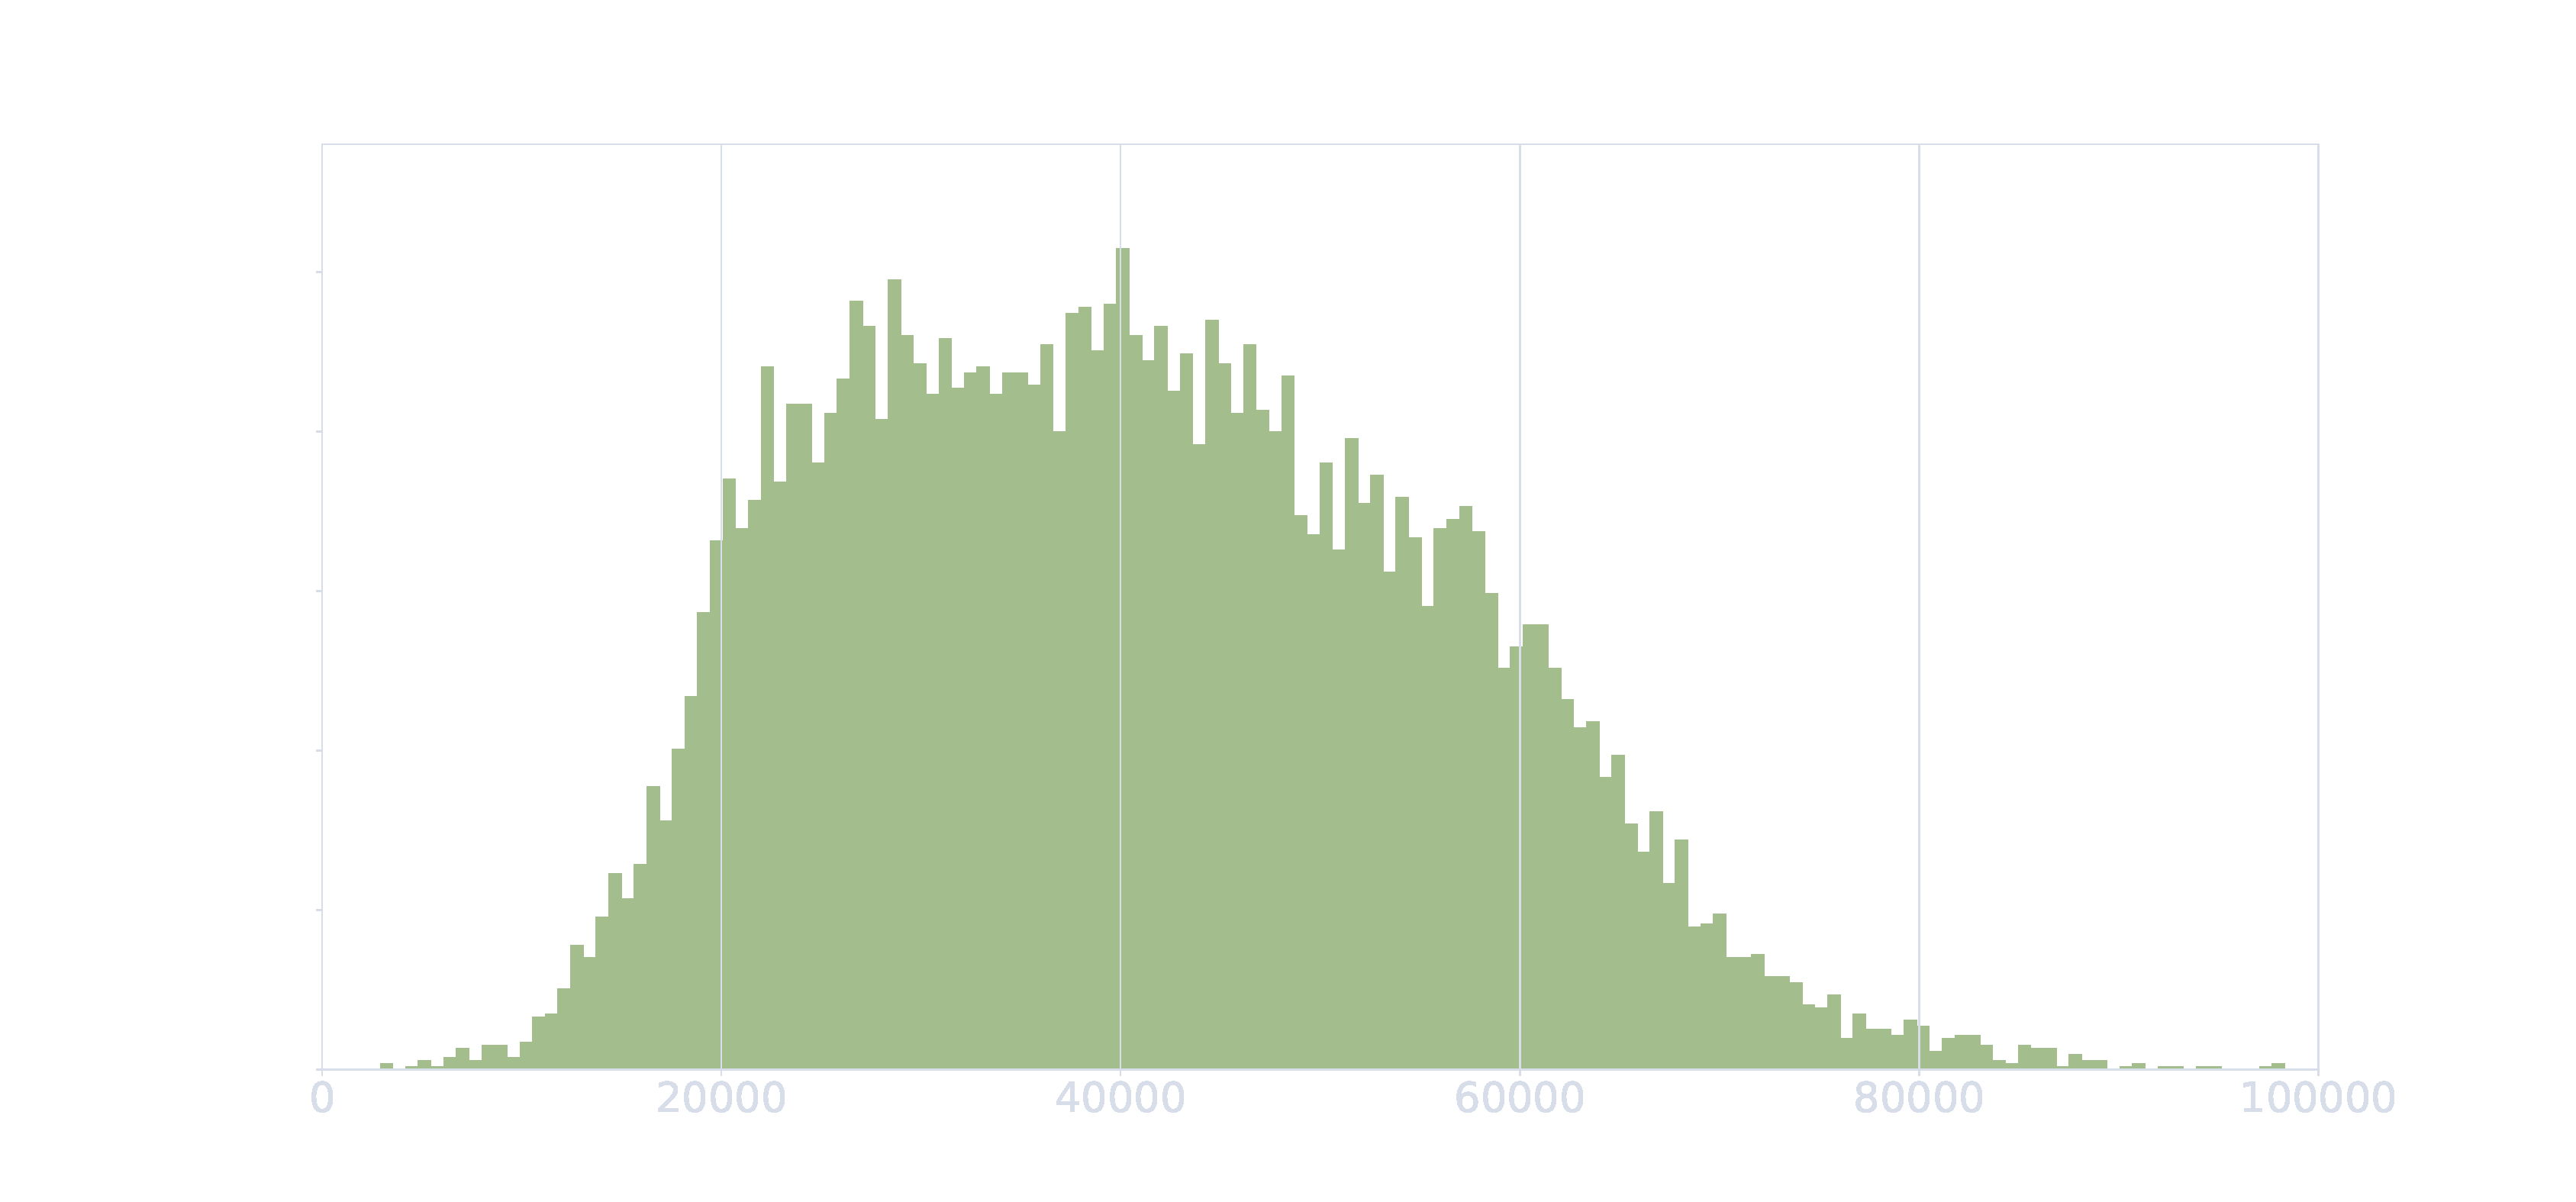
\includegraphics[width=\textwidth]{sc_violations_hist.pdf}
	\end{figure}
\end{frame}

\begin{frame}[fragile]{Program order}{Compiler barrier}
	\begin{columns}[T]
			\begin{column}{0.45\textwidth}
\begin{lstlisting}[title={Thread 1}]
void thread_1_body ()
{
  x = 1;
  asm volatile (
    "mfence" ::: "memory");
  r1 = y;
}
\end{lstlisting}
\end{column}

\begin{column}{0.45\textwidth}
\begin{lstlisting}[title={Thread 2}]
void thread_2_body ()
{
  y = 1;
  asm volatile (
    "mfence" ::: "memory");
  r2 = x;
}
\end{lstlisting}
			\end{column}
	\end{columns}

\end{frame}

\begin{frame}[fragile]{Weak models}{definitions}
\begin{description}[Weak memory models]
\item[Weak memory models] preserves only the orders that programmers require.
\item[memory operations] can be reordered unless there is a \textcolor{NordYellow}{fence} between them.
	\begin{itemize}
		\item $L(a) \mathbin{\color{NordYellow}\mathord{<}p} \textnormal{FENCE} \Rightarrow L(a) \mathbin{\color{NordYellow}\mathord{<}m} \textnormal{FENCE}$
		\item $S(a) \mathbin{\color{NordYellow}\mathord{<}p} \textnormal{FENCE} \Rightarrow S(a) \mathbin{\color{NordYellow}\mathord{<}m} \textnormal{FENCE}$
		\item $\textnormal{FENCE} \mathbin{\color{NordYellow}\mathord{<}p} L(a) \Rightarrow \textnormal{FENCE} \mathbin{\color{NordYellow}\mathord{<}m} L(a)$
		\item $\textnormal{FENCE} \mathbin{\color{NordYellow}\mathord{<}p} S(a) \Rightarrow \textnormal{FENCE} \mathbin{\color{NordYellow}\mathord{<}m} S(a)$
	\end{itemize}
\end{description}
\end{frame}

\begin{frame}[fragile]{Operations interleaving}{}
\begin{columns}[T]
	\begin{column}{0.4\textwidth}
\begin{lstlisting}[]
__device__ void writer (
    volatile int * v1,
    volatile int * v2,
    volatile int * v3,
    volatile int * v4)
{
  *v1 = 1;
  *v2 = 2;
  *v3 = 3;
  *v4 = 4;
}
\end{lstlisting}
\end{column}

\begin{column}{0.45\textwidth}
\begin{lstlisting}[]
__device__ void reader (
    volatile int * v1,
    volatile int * v2,
    volatile int * v3,
    volatile int * v4,
    int *result)
{
  int r1 = *v1; int r2 = *v2;
  int r3 = *v3; int r4 = *v4;

  if (   r1 == 1 && r3 == 3 
      && r2 == 0 && r4 == 0)
    *result = 0;
}
\end{lstlisting}
			\end{column}
	\end{columns}
\end{frame}

\begin{frame}[fragile]{Operations interleaving}{TSO}
	\begin{figure}
	\centering
		\begin{tikzpicture}
			\begin{sankeydiagram}[
				sankey tot length=60pt,%
				sankey tot quantity=12,%
				sankey min radius=15pt,%
				sankey fill/.style={
					draw,line width=0pt,
					fill,
					NordGreen,
				},
				sankey draw/.style={
					draw=white, %NordBlack,
					line width=1pt,
					line cap=round,
					line join=round,
				},
				%	sankey debug,
				]

				% First thread
				\sankeynode{12}{0}{t0i0}{0,0};
				\sankeyadvance{t0i0}{45pt}

				\sankeyfork{t0i0}{3/p1,3/p2,3/p3,3/p4}

				% \sankeyturn{p1}{20}
				% \sankeyadvance{p2}{20pt}

				\sankeynode{3}{0}{p11a}{[shift={(30pt,52.5pt)}]t0i0}
				\sankeynode{3}{0}{p12a}{[shift={(30pt,37.5pt)}]t0i0}
				\sankeynode{3}{0}{p13a}{[shift={(30pt,-37.5pt)}]t0i0}
				\sankeynode{3}{0}{p14a}{[shift={(30pt,-52.5pt)}]t0i0}
				\path (p1) to[sankey flow] (p11a);
				\path (p2) to[sankey flow] (p13a);
				\path (p3) to[sankey flow] (p12a);
				\path (p4) to[sankey flow] (p14a);

				\node[anchor=west,text=NordDarkBlack] at ([shift={(-45pt,0pt)}]p1) {*v1 = 1};
				\node[anchor=west,text=NordDarkBlack] at ([shift={(-45pt,0pt)}]p2) {*v2 = 2};
				\node[anchor=west,text=NordDarkBlack] at ([shift={(-45pt,0pt)}]p3) {*v3 = 3};
				\node[anchor=west,text=NordDarkBlack] at ([shift={(-45pt,0pt)}]p4) {*v4 = 4};

				\node[anchor=east] (p11as) at (p11a) {};
				\node[anchor=east] (p12as) at (p12a) {};
				\node[anchor=east] (p13as) at (p13a) {};
				\node[anchor=east] (p14as) at (p14a) {};

				\sankeyadvance{p11a}{55pt}
				\sankeyadvance{p12a}{55pt}
				\sankeyadvance{p13a}{55pt}
				\sankeyadvance{p14a}{55pt}

				\node[anchor=west,text=NordDarkBlack] at ([shift={(8pt,0pt)}]p11as) {store v1};
				\node[anchor=west,text=NordDarkBlack] at ([shift={(8pt,0pt)}]p12as) {store v3};
				\node[anchor=west,text=NordDarkBlack] at ([shift={(8pt,0pt)}]p13as) {store v2};
				\node[anchor=west,text=NordDarkBlack] at ([shift={(8pt,0pt)}]p14as) {store v4};


			% Second thread
			{
				\tikzset{
					sankey fill/.append style={
						draw,line width=0pt,
						fill,
						NordBlue,
					}
				}
				\sankeynode{12}{180}{t1i0}{[shift={(155pt,0pt)}]t0i0};
				\sankeyadvance{t1i0}{45pt}
				\sankeyfork{t1i0}{3/p5,3/p6,3/p7,3/p8}

				\sankeynode{3}{180}{p15a}{[shift={(85pt,22.5pt)}]t0i0}
				\sankeynode{3}{180}{p14a}{[shift={(85pt,7.5pt)}]t0i0}
				\sankeynode{3}{180}{p16a}{[shift={(85pt,-7.5pt)}]t0i0}
				\sankeynode{3}{180}{p17a}{[shift={(85pt,-22.5pt)}]t0i0}
				\path (p7) to[sankey flow] (p14a);
				\path (p8) to[sankey flow] (p15a);
				\path (p6) to[sankey flow] (p16a);
				\path (p5) to[sankey flow] (p17a);
				\sankeyadvance{p14a}{55pt}
				\sankeyadvance{p15a}{55pt}
				\sankeyadvance{p16a}{55pt}
				\sankeyadvance{p17a}{55pt}

				\node[anchor=west,text=NordDarkBlack] at ([shift={(4pt,0pt)}]p14a) {load v2};
				\node[anchor=west,text=NordDarkBlack] at ([shift={(4pt,0pt)}]p15a) {load v1};
				\node[anchor=west,text=NordDarkBlack] at ([shift={(4pt,0pt)}]p16a) {load v3};
				\node[anchor=west,text=NordDarkBlack] at ([shift={(4pt,0pt)}]p17a) {load v4};

				\node[anchor=west,text=NordDarkBlack] at (p5) {r4 = v4};
				\node[anchor=west,text=NordDarkBlack] at (p6) {r3 = v3};
				\node[anchor=west,text=NordDarkBlack] at (p7) {r2 = v2};
				\node[anchor=west,text=NordDarkBlack] at (p8) {r1 = v1};
			}

				\draw [densely dashed,thick,draw=NordWhite] (0pt,60pt) -- (0pt,-95pt);
				\draw [densely dashed,thick,draw=NordWhite] (75pt,60pt) -- (75pt,-95pt);
				\draw [densely dashed,thick,draw=NordWhite] (130pt,60pt) -- (130pt,-95pt);
				\draw [densely dashed,thick,draw=NordWhite] (200pt,60pt) -- (200pt,-95pt);

				\node[text=NordWhite,text width=4cm,align=center,anchor=center] at (38pt,-80pt) {\small Writer};
				\node[text=NordWhite,text width=4cm,align=center,anchor=center] at (102pt,-80pt) {\small Memory\\order};
				\node[text=NordWhite,text width=4cm,align=center,anchor=center] at (166pt,-80pt) {\small Reader};
			\end{sankeydiagram}
		\end{tikzpicture}
	\end{figure}
\end{frame}


\begin{frame}[fragile]{Operations interleaving}{}

Was interleaved up to \textbf{671} times out of 1000 runs on RTX 3090.

\begin{columns}[T]
	\begin{column}{0.4\textwidth}
		\begin{lstlisting}[title={Writer},language={SASS}]
IMAD.MOV.U32 R0, RZ, RZ, 0x1;
IMAD.MOV.U32 R2, RZ, RZ, 0x2;
IMAD.MOV.U32 R3, RZ, RZ, 0x3;
IMAD.MOV.U32 R4, RZ, RZ, 0x4;
STG.E.STRONG.SYS [UR4], R0;
STG.E.STRONG.SYS [UR6], R2;
STG.E.STRONG.SYS [UR8], R3;
STG.E.STRONG.SYS [UR10], R4;
\end{lstlisting}
\end{column}

\begin{column}{0.45\textwidth}
\begin{lstlisting}[title={Reader},language={SASS}]
LDG.E.STRONG.SYS R0, [UR4];
LDG.E.STRONG.SYS R2, [UR6];
LDG.E.STRONG.SYS R3, [UR8];
LDG.E.STRONG.SYS R4, [UR10];
\end{lstlisting}
			\end{column}
	\end{columns}

\end{frame}

\begin{frame}[fragile]{Operations interleaving}{}
\centering
\begin{lstlisting}
  cudaMemset (x, 0, 4 * sizeof (int));
  cudaMemset (y, 0, 2 * sizeof (int));

  if (single_segment)
    kernel<<<1024, 32>>> (x + 0, x + 1, x + 2, x + 3, r);
  else
    kernel<<<1024, 32>>> (x + 0, y + 0, x + 1, y + 1, r);
\end{lstlisting}
\end{frame}


\begin{frame}[fragile]{Write Buffer}{}
\centering
\begin{columns}[T]
	\begin{column}{0.4\textwidth}
\begin{lstlisting}[]
__host__ void writer (
    volatile int * v1,
    volatile int * v2,
    volatile int * v3,
    volatile int * v4)
{          // <=
  *v1 = 1;
  *v2 = 2;
  *v3 = 3;
  *v4 = 4;
}
\end{lstlisting}
\end{column}
\begin{column}{0.4\textwidth}
	\centering
	Entry: single word
	\begin{table}
		\begin{tabular}{| c | c |}
			\hline 
			addr & value \\
			\hline 
			\textcolor{NordBlack}{200} & \textcolor{NordBlack}{value} \\
			\hline 
			\textcolor{NordBlack}{400} & \textcolor{NordBlack}{value} \\
			\hline 
			\textcolor{NordBlack}{204} & \textcolor{NordBlack}{value} \\
			\hline 
			\textcolor{NordBlack}{404} & \textcolor{NordBlack}{value} \\
			\hline 
		\end{tabular}
	\end{table}
\end{column}
\end{columns}
\end{frame}


\begin{frame}[fragile]{Write Buffer}{}
\centering
\begin{columns}[T]
	\begin{column}{0.4\textwidth}
\begin{lstlisting}[]
__host__ void writer (
    volatile int * v1,
    volatile int * v2,
    volatile int * v3,
    volatile int * v4)
{          
  *v1 = 1; // <=
  *v2 = 2;
  *v3 = 3;
  *v4 = 4;
}
\end{lstlisting}
\end{column}
\begin{column}{0.4\textwidth}
	\centering
	Entry: single word
	\begin{table}
		\begin{tabular}{| c | c |}
			\hline 
			addr & value \\
			\hline 
			200 & 1 \\
			\hline 
			\textcolor{NordBlack}{400} & \textcolor{NordBlack}{value} \\
			\hline 
			\textcolor{NordBlack}{204} & \textcolor{NordBlack}{value} \\
			\hline 
			\textcolor{NordBlack}{404} & \textcolor{NordBlack}{value} \\
			\hline 
		\end{tabular}
	\end{table}
\end{column}
\end{columns}
\end{frame}


\begin{frame}[fragile]{Write Buffer}{}
\centering
\begin{columns}[T]
	\begin{column}{0.4\textwidth}
\begin{lstlisting}[]
__host__ void writer (
    volatile int * v1,
    volatile int * v2,
    volatile int * v3,
    volatile int * v4)
{          
  *v1 = 1;
  *v2 = 2; // <=
  *v3 = 3;
  *v4 = 4;
}
\end{lstlisting}
\end{column}
\begin{column}{0.4\textwidth}
	\centering
	Entry: single word
	\begin{table}
		\begin{tabular}{| c | c |}
			\hline 
			addr & value \\
			\hline 
			200 & 1 \\
			\hline 
			400 & 2 \\
			\hline 
			\textcolor{NordBlack}{204} & \textcolor{NordBlack}{value} \\
			\hline 
			\textcolor{NordBlack}{404} & \textcolor{NordBlack}{value} \\
			\hline 
		\end{tabular}
	\end{table}
\end{column}
\end{columns}
\end{frame}


\begin{frame}[fragile]{Write Buffer}{}
\centering
\begin{columns}[T]
	\begin{column}{0.4\textwidth}
\begin{lstlisting}[]
__host__ void writer (
    volatile int * v1,
    volatile int * v2,
    volatile int * v3,
    volatile int * v4)
{          
  *v1 = 1;
  *v2 = 2;
  *v3 = 3; // <=
  *v4 = 4;
}
\end{lstlisting}
\end{column}
\begin{column}{0.4\textwidth}
	\centering
	Entry: single word
	\begin{table}
		\begin{tabular}{| c | c |}
			\hline 
			addr & value \\
			\hline 
			200 & 1 \\
			\hline 
			400 & 2 \\
			\hline 
			204 & 3 \\
			\hline 
			\textcolor{NordBlack}{404} & \textcolor{NordBlack}{value} \\
			\hline 
		\end{tabular}
	\end{table}
\end{column}
\end{columns}
\end{frame}

\begin{frame}[fragile]{Write Buffer}{}
\centering
\begin{columns}[T]
	\begin{column}{0.4\textwidth}
\begin{lstlisting}[]
__host__ void writer (
    volatile int * v1,
    volatile int * v2,
    volatile int * v3,
    volatile int * v4)
{          
  *v1 = 1;
  *v2 = 2;
  *v3 = 3;
  *v4 = 4; // <=
}
\end{lstlisting}
\end{column}
\begin{column}{0.4\textwidth}
	\centering
	Entry: single word
	\begin{table}
		\begin{tabular}{| c | c |}
			\hline 
			addr & value \\
			\hline 
			200 & 1 \\
			\hline 
			400 & 2 \\
			\hline 
			204 & 3 \\
			\hline 
			404 & 4 \\
			\hline 
		\end{tabular}
	\end{table}
\end{column}
\end{columns}
\end{frame}


\begin{frame}[fragile]{Merging Write Buffer}{}
\centering
\begin{columns}[T]
	\begin{column}{0.4\textwidth}
\begin{lstlisting}[]
__device__ void writer (
    volatile int * v1,
    volatile int * v2,
    volatile int * v3,
    volatile int * v4)
{          // <= 
  *v1 = 1;
  *v2 = 2;
  *v3 = 3;
  *v4 = 4;
}
\end{lstlisting}
\end{column}
\begin{column}{0.5\textwidth}
	\centering
	Entry: cache block
	\begin{table}
		\begin{tabular}{| c | c | c | c | c |}
			\hline 
			addr & value & value & value & value  \\
			\hline 
			\textcolor{NordBlack}{200} & \textcolor{NordBlack}{1} & & & \\
			\hline 
			\textcolor{NordBlack}{200} & \textcolor{NordBlack}{1} & & & \\
			\hline 
		\end{tabular}
	\end{table}
\end{column}
\end{columns}
\end{frame}


\begin{frame}[fragile]{Merging Write Buffer}{}
\centering
\begin{columns}[T]
	\begin{column}{0.4\textwidth}
\begin{lstlisting}[]
__device__ void writer (
    volatile int * v1,
    volatile int * v2,
    volatile int * v3,
    volatile int * v4)
{          
  *v1 = 1; // <= 
  *v2 = 2;
  *v3 = 3;
  *v4 = 4;
}
\end{lstlisting}
\end{column}
\begin{column}{0.5\textwidth}
	\centering
	Entry: cache block
	\begin{table}
		\begin{tabular}{| c | c | c | c | c |}
			\hline 
			addr & value & value & value & value  \\
			\hline 
			200 & 1 & & & \\
			\hline 
			\textcolor{NordBlack}{200} & \textcolor{NordBlack}{1} & & & \\
			\hline 
		\end{tabular}
	\end{table}
\end{column}
\end{columns}
\end{frame}


\begin{frame}[fragile]{Merging Write Buffer}{}
\centering
\begin{columns}[T]
	\begin{column}{0.4\textwidth}
\begin{lstlisting}[]
__device__ void writer (
    volatile int * v1,
    volatile int * v2,
    volatile int * v3,
    volatile int * v4)
{          
  *v1 = 1;
  *v2 = 2; // <= 
  *v3 = 3;
  *v4 = 4;
}
\end{lstlisting}
\end{column}
\begin{column}{0.5\textwidth}
	\centering
	Entry: cache block
	\begin{table}
		\begin{tabular}{| c | c | c | c | c |}
			\hline 
			addr & value & value & value & value  \\
			\hline 
			200 & 1 & & & \\
			\hline 
			400 & 2 & & & \\
			\hline 
		\end{tabular}
	\end{table}
\end{column}
\end{columns}
\end{frame}


\begin{frame}[fragile]{Merging Write Buffer}{}
\centering
\begin{columns}[T]
	\begin{column}{0.4\textwidth}
\begin{lstlisting}[]
__device__ void writer (
    volatile int * v1,
    volatile int * v2,
    volatile int * v3,
    volatile int * v4)
{          
  *v1 = 1;
  *v2 = 2;
  *v3 = 3; // <= 
  *v4 = 4;
}
\end{lstlisting}
\end{column}
\begin{column}{0.5\textwidth}
	\centering
	Entry: cache block
	\begin{table}
		\begin{tabular}{| c | c | c | c | c |}
			\hline 
			addr & value & value & value & value  \\
			\hline 
			200 & 1 & 3 & & \\
			\hline 
			400 & 2 & & & \\
			\hline 
		\end{tabular}
	\end{table}
\end{column}
\end{columns}
\end{frame}


\begin{frame}[fragile]{Merging Write Buffer}{}
\centering
\begin{columns}[T]
	\begin{column}{0.4\textwidth}
\begin{lstlisting}[]
__device__ void writer (
    volatile int * v1,
    volatile int * v2,
    volatile int * v3,
    volatile int * v4)
{          
  *v1 = 1;
  *v2 = 2;
  *v3 = 3;
  *v4 = 4; // <= 
}
\end{lstlisting}
\end{column}
\begin{column}{0.5\textwidth}
	\centering
	Entry: cache block
	\begin{table}
		\begin{tabular}{| c | c | c | c | c |}
			\hline 
			addr & value & value & value & value  \\
			\hline 
			200 & 1 & 3 & & \\
			\hline 
			400 & 2 & 4 & & \\
			\hline 
		\end{tabular}
	\end{table}
\end{column}
\end{columns}
\end{frame}


\begin{frame}[fragile]{Operations interleaving}{fixed version}
\begin{columns}[T]
	\begin{column}{0.4\textwidth}
\begin{lstlisting}[]
__device__ void writer (
    volatile int * v1,
    volatile int * v2,
    volatile int * v3,
    volatile int * v4)
{
  *v1 = 1;
  *v2 = 2;
  __threadfence ();
  *v3 = 3;
  *v4 = 4;
}
\end{lstlisting}
\end{column}

\begin{column}{0.45\textwidth}
\begin{lstlisting}[]
__device__ void reader (
    volatile int * v1,
    volatile int * v2,
    volatile int * v3,
    volatile int * v4,
    int *result)
{
  int r1 = *v1; int r2 = *v2;
  __threadfence ();
  int r3 = *v3; int r4 = *v4;

  if (   r1 == 1 && r3 == 3 
      && r2 == 0 && r4 == 0)
    *result = 0;
}
\end{lstlisting}
			\end{column}
	\end{columns}
\end{frame}


\begin{frame}[fragile]{Operations interleaving}{RTX 3090}
\centering
	\begin{figure}
		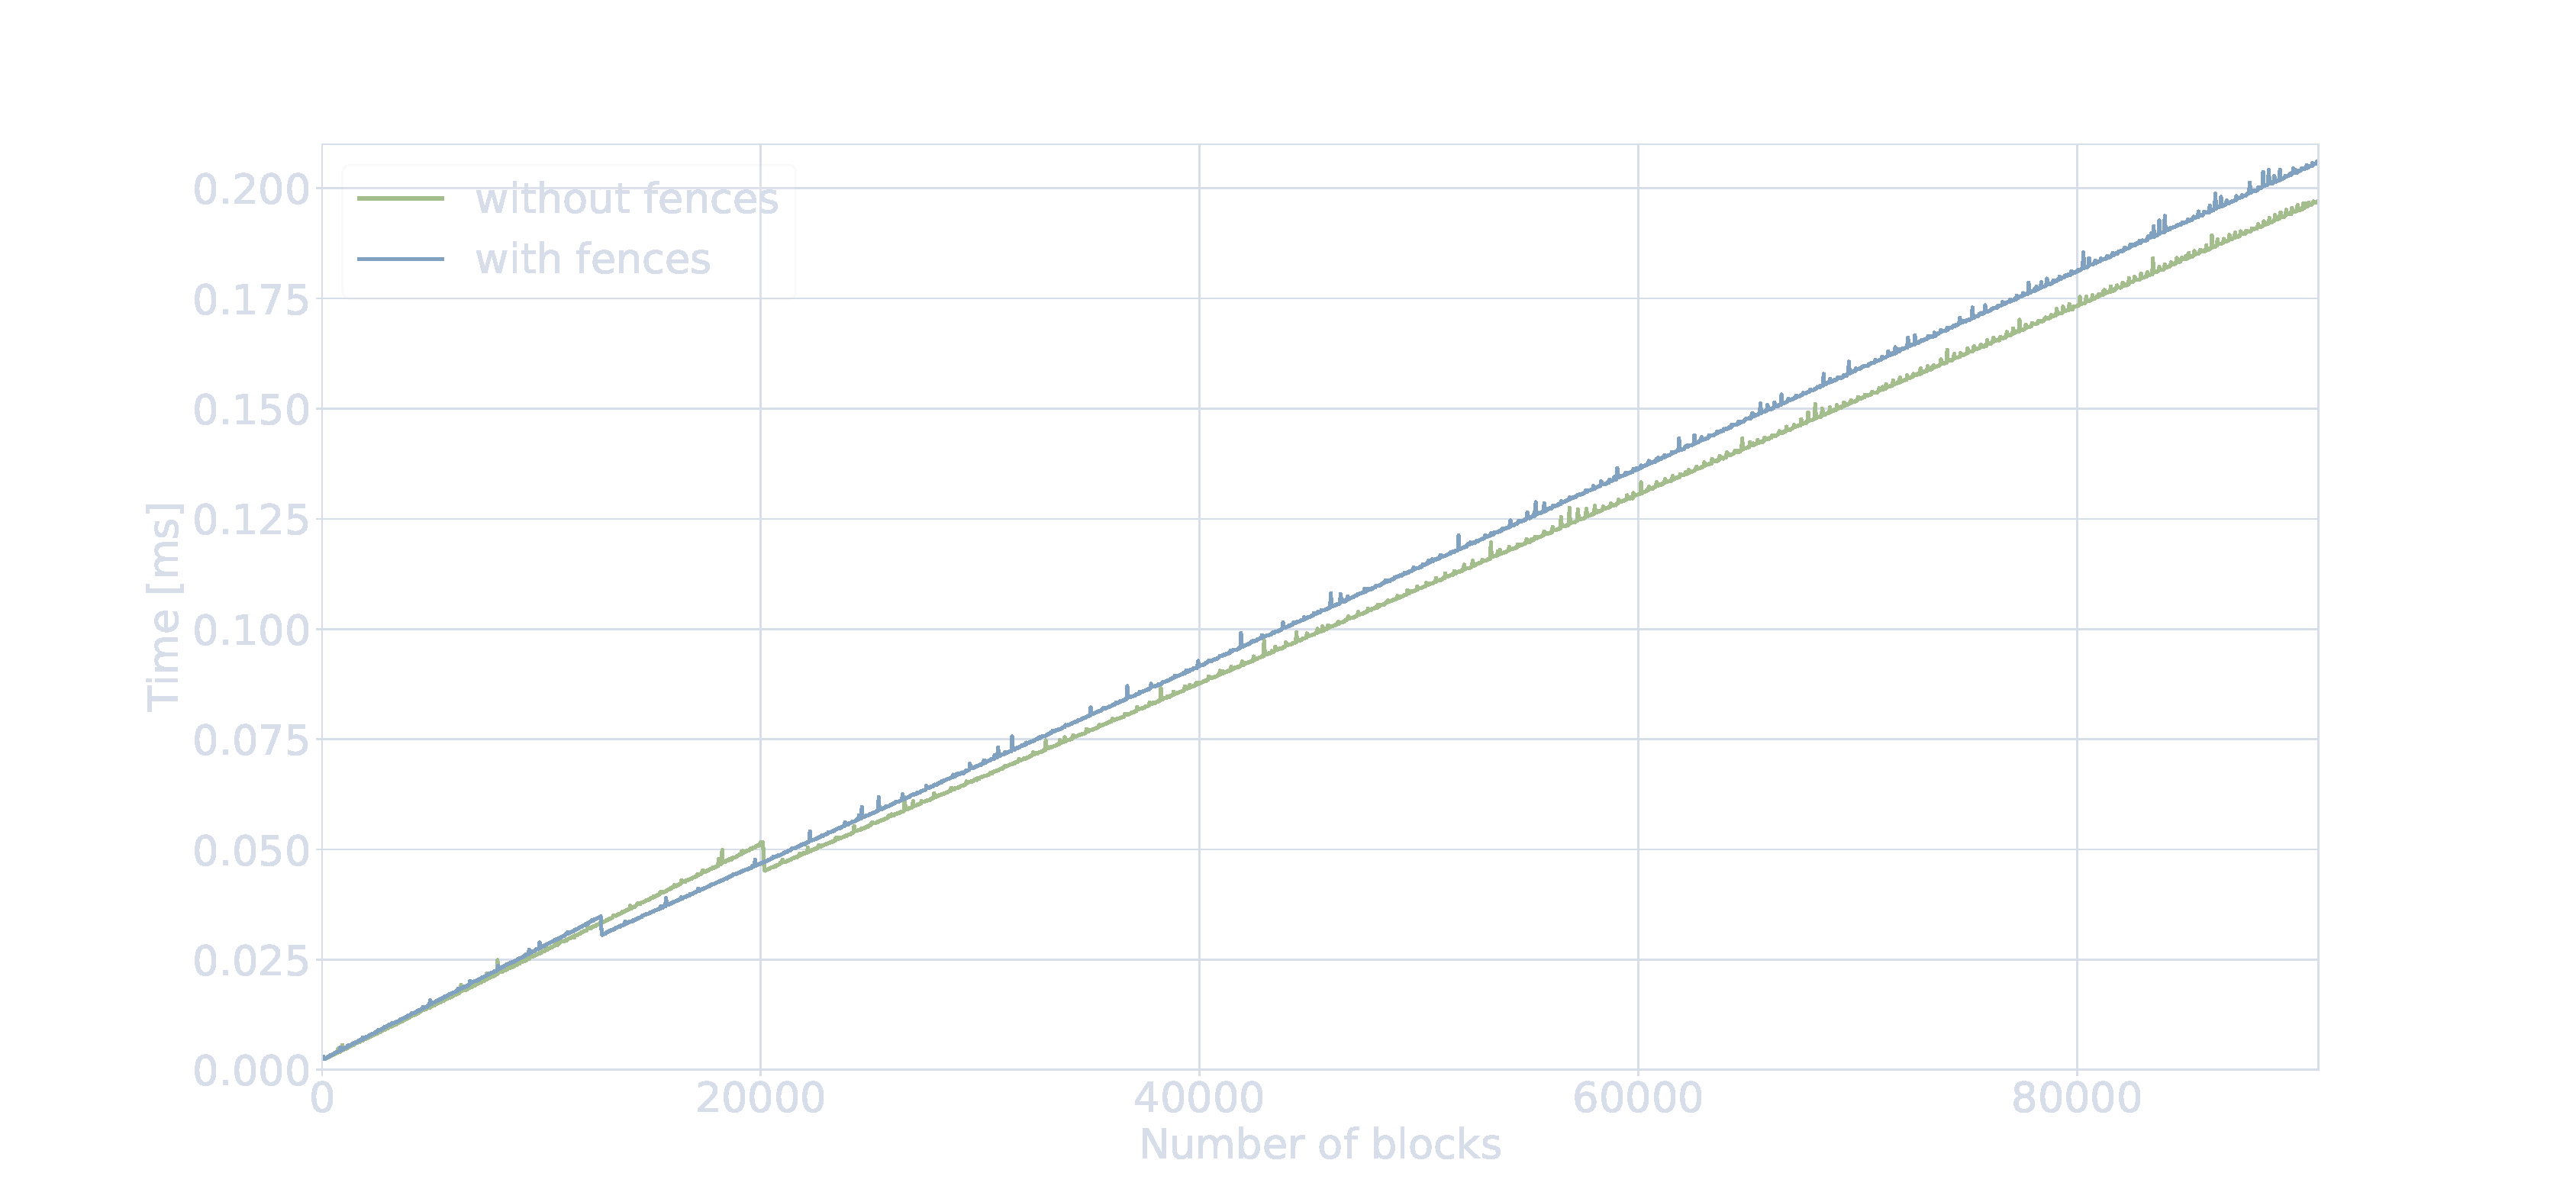
\includegraphics[width=\textwidth]{interleaved_fence_perf.pdf}
	\end{figure}
\end{frame}


\begin{frame}[fragile]{Read-Read Coherence}{coRR}
\centering
\begin{lstlisting}
__global__ void coherence_of_read_read (/*...*/) {
  __shared__ int cache[BLOCK_SIZE];
  /* .. Initialize shared memory .. */
  __syncthreads ();
  if (tid == wthread) {
    cache[tid] = 1;
  }
  else {
    const int r1 = cache[reordering_1[tid]]; 
    const int r2 = cache[reordering_2[tid]];
    if (r1 == 1 && r2 == 0) 
      if (tid == rthread) 
        *violated = 1;
  }
}     
\end{lstlisting}
\end{frame}

\begin{frame}[fragile]{Read-Read Coherence}{coRR}
	\begin{figure}
	\centering
		\begin{tikzpicture}
			\begin{sankeydiagram}[
				sankey tot length=30pt,%
				sankey tot quantity=6,%
				sankey min radius=15pt,%
				sankey fill/.style={
					draw,line width=0pt,
					fill,
					NordGreen,
				},
				sankey draw/.style={
					draw=white, %NordBlack,
					line width=1pt,
					line cap=round,
					line join=round,
				},
				%	sankey debug,
				]

				% First thread
				\sankeynode{3}{0}{t0i0}{0,0};
				\sankeyadvance{t0i0}{60pt}

				% \sankeyturn{p1}{20}
				% \sankeyadvance{p2}{20pt}

				\sankeynode{3}{0}{p11a}{[shift={(15pt,22.5pt)}]t0i0}
				\path (t0i0) to[sankey flow] (p11a);

				\node[anchor=west,text=NordDarkBlack] at (0,0) {x = 1};

				\node[anchor=east] (p11as) at (p11a) {};

				\sankeyadvance{p11a}{55pt}

				\node[anchor=west,text=NordDarkBlack] at ([shift={(8pt,0pt)}]p11as) {store x};


			% Second thread
			{
				\tikzset{
					sankey fill/.append style={
						draw,line width=0pt,
						fill,
						NordBlue,
					}
				}
				\sankeynode{6}{180}{t1i0}{[shift={(142pt,0pt)}]t0i0};
				\sankeyadvance{t1i0}{57pt}
				\sankeyfork{t1i0}{3/p3,3/p4}

				\sankeynode{3}{180}{p15a}{[shift={(70pt,-7.5pt)}]t0i0}
				\sankeynode{3}{180}{p14a}{[shift={(70pt,7.5pt)}]t0i0}
				\path (p4) to[sankey flow] (p15a);
				\path (p3) to[sankey flow] (p14a);
				\sankeyadvance{p14a}{55pt}
				\sankeyadvance{p15a}{55pt}

				\node[anchor=west,text=NordDarkBlack] at ([shift={(4pt,0pt)}]p14a) {load x};
				\node[anchor=west,text=NordDarkBlack] at ([shift={(4pt,0pt)}]p15a) {load x};

				\node[anchor=west,text=NordDarkBlack] at (145pt,0.25) {r1 = x};
				\node[anchor=west,text=NordDarkBlack] at (145pt,-0.25) {r2 = x};
			}

				\draw [densely dashed,thick,draw=NordWhite] (0pt,30pt) -- (0pt,-55pt);
				\draw [densely dashed,thick,draw=NordWhite] (75pt,30pt) -- (75pt,-55pt);
				\draw [densely dashed,thick,draw=NordWhite] (130pt,30pt) -- (130pt,-55pt);
				\draw [densely dashed,thick,draw=NordWhite] (202pt,30pt) -- (202pt,-55pt);

				\node[text=NordWhite,text width=4cm,align=center,anchor=center] at (38pt,-40pt) {\small Thread 1\\program order};
				\node[text=NordWhite,text width=4cm,align=center,anchor=center] at (102pt,-40pt) {\small Memory\\order};
				\node[text=NordWhite,text width=4cm,align=center,anchor=center] at (166pt,-40pt) {\small Thread 2\\program order};
			\end{sankeydiagram}
		\end{tikzpicture}
	\end{figure}
\end{frame}

\begin{frame}[fragile]{Read-Read Coherence}{coRR}

Violated \textbf{157} times out of 100'000 runs on GTX 560 (Fermi). Fixed in Maxwell.

\begin{columns}
	\begin{column}{0.3\textwidth}
\begin{lstlisting}[language={SASS},title={Thread 1}]
MOV32I R0, 0x1;
STS [R7], R0;
\end{lstlisting}

	\end{column}
	\begin{column}{0.6\textwidth}
		\begin{lstlisting}[language={SASS},title={Thread 2}]
LDS R0, [R0];
LDS R4, [R4]; /* [R4] = [R0] */
ISETP.EQ.AND P0, PT, R0, 0x1, PT;
ISETP.EQ.AND P0, PT, R4, RZ, P0;
\end{lstlisting}
	\end{column}
	\end{columns}

\end{frame}

\begin{frame}[fragile]{Message Passing}{}
\centering
\begin{lstlisting}
__global__ void kernel (
    int n, int * flag, int * data, int *result) { 
\end{lstlisting}

\begin{columns}[T]
	\begin{column}{0.45\textwidth}
\begin{lstlisting}[title={Writer}]
for (int i = 0; i < n; i++)
  data[i] = i + 1;

*flag = 1;
\end{lstlisting}
\end{column}

\begin{column}{0.45\textwidth}
\begin{lstlisting}[title={Reader}]
while (*flag == 0);

for (int i = 0; i < n; i++)
  if (data[i] == 0)
    *result = 0;
\end{lstlisting}
			\end{column}
	\end{columns}
\end{frame}

\begin{frame}[fragile]{Message Passing}{}
\centering
\begin{lstlisting}
__global__ void kernel (
    int n, int * flag, int * data, int *result) { 
\end{lstlisting}

\begin{columns}[T]
	\begin{column}{0.45\textwidth}
\begin{lstlisting}[title={Writer}]
for (int i = 0; i < n; i++)
  data[i] = i + 1;

*flag = 1;
\end{lstlisting}
\end{column}

\begin{column}{0.45\textwidth}
\begin{lstlisting}[language={SASS},title={SASS}]
IADD R3, R0, 0x1;
IADD R4, R0, 0x2;
STG.E [R1], R3
IADD R3, R0, 0x3;
STG.E [R2], R4;
; /* ... */
MOV32I R5, 0x1;
STG.E [flag], R5;
\end{lstlisting}
\end{column}
	\end{columns}
\end{frame}

\begin{frame}[fragile]{Message Passing}{}
\centering
\begin{lstlisting}
__global__ void kernel (
    int n, int * flag, int * data, int *result) { 
\end{lstlisting}

\begin{columns}[T]
	\begin{column}{0.45\textwidth}
\begin{lstlisting}[title={Reader}]
while (*flag == 0);

for (int i = 0; i < n; i++)
  if (data[i] == 0)
    *result = 0;
\end{lstlisting}
\end{column}

\begin{column}{0.45\textwidth}
\begin{lstlisting}[language={SASS},title={SASS}]
LDG.E R1, [R0];
ISETP.NE.AND P0, PT, R2, RZ, PT;
@!P0 BRA .L1;
LDG.E R3, [R2];
LDG.E R4, [R2+0x4];
LDG.E R5, [R2+0x8];
LDG.E R6, [R2+0xc];
; /* ... */
EXIT;
.L1:
BRA .L1;
\end{lstlisting}
\end{column}
	\end{columns}
\end{frame}

\begin{frame}[fragile]{Message Passing}{first fix}
\centering
\begin{lstlisting}
__global__ void kernel (
    int n, volatile int * flag, int * data, int *result) { 
\end{lstlisting}

\begin{columns}[T]
	\begin{column}{0.45\textwidth}
\begin{lstlisting}[title={Reader}]
while (*flag == 0);

for (int i = 0; i < n; i++)
  if (data[i] == 0)
    *result = 0;
\end{lstlisting}
\end{column}

\begin{column}{0.45\textwidth}
\begin{lstlisting}[language={SASS},title={SASS}]
.L1:
LDG.E.STRONG.SYS R1, [R0];
ISETP.NE.AND P0, PT, R2, RZ, PT;
@!P0 BRA .L1;
LDG.E R3, [R2];
LDG.E R4, [R2+0x4];
LDG.E R5, [R2+0x8];
LDG.E R6, [R2+0xc];
; /* ... */
EXIT;
\end{lstlisting}
\end{column}
	\end{columns}
\end{frame}

\begin{frame}[fragile]{Stale data found}{RTX 2080}
\centering
	\begin{figure}
		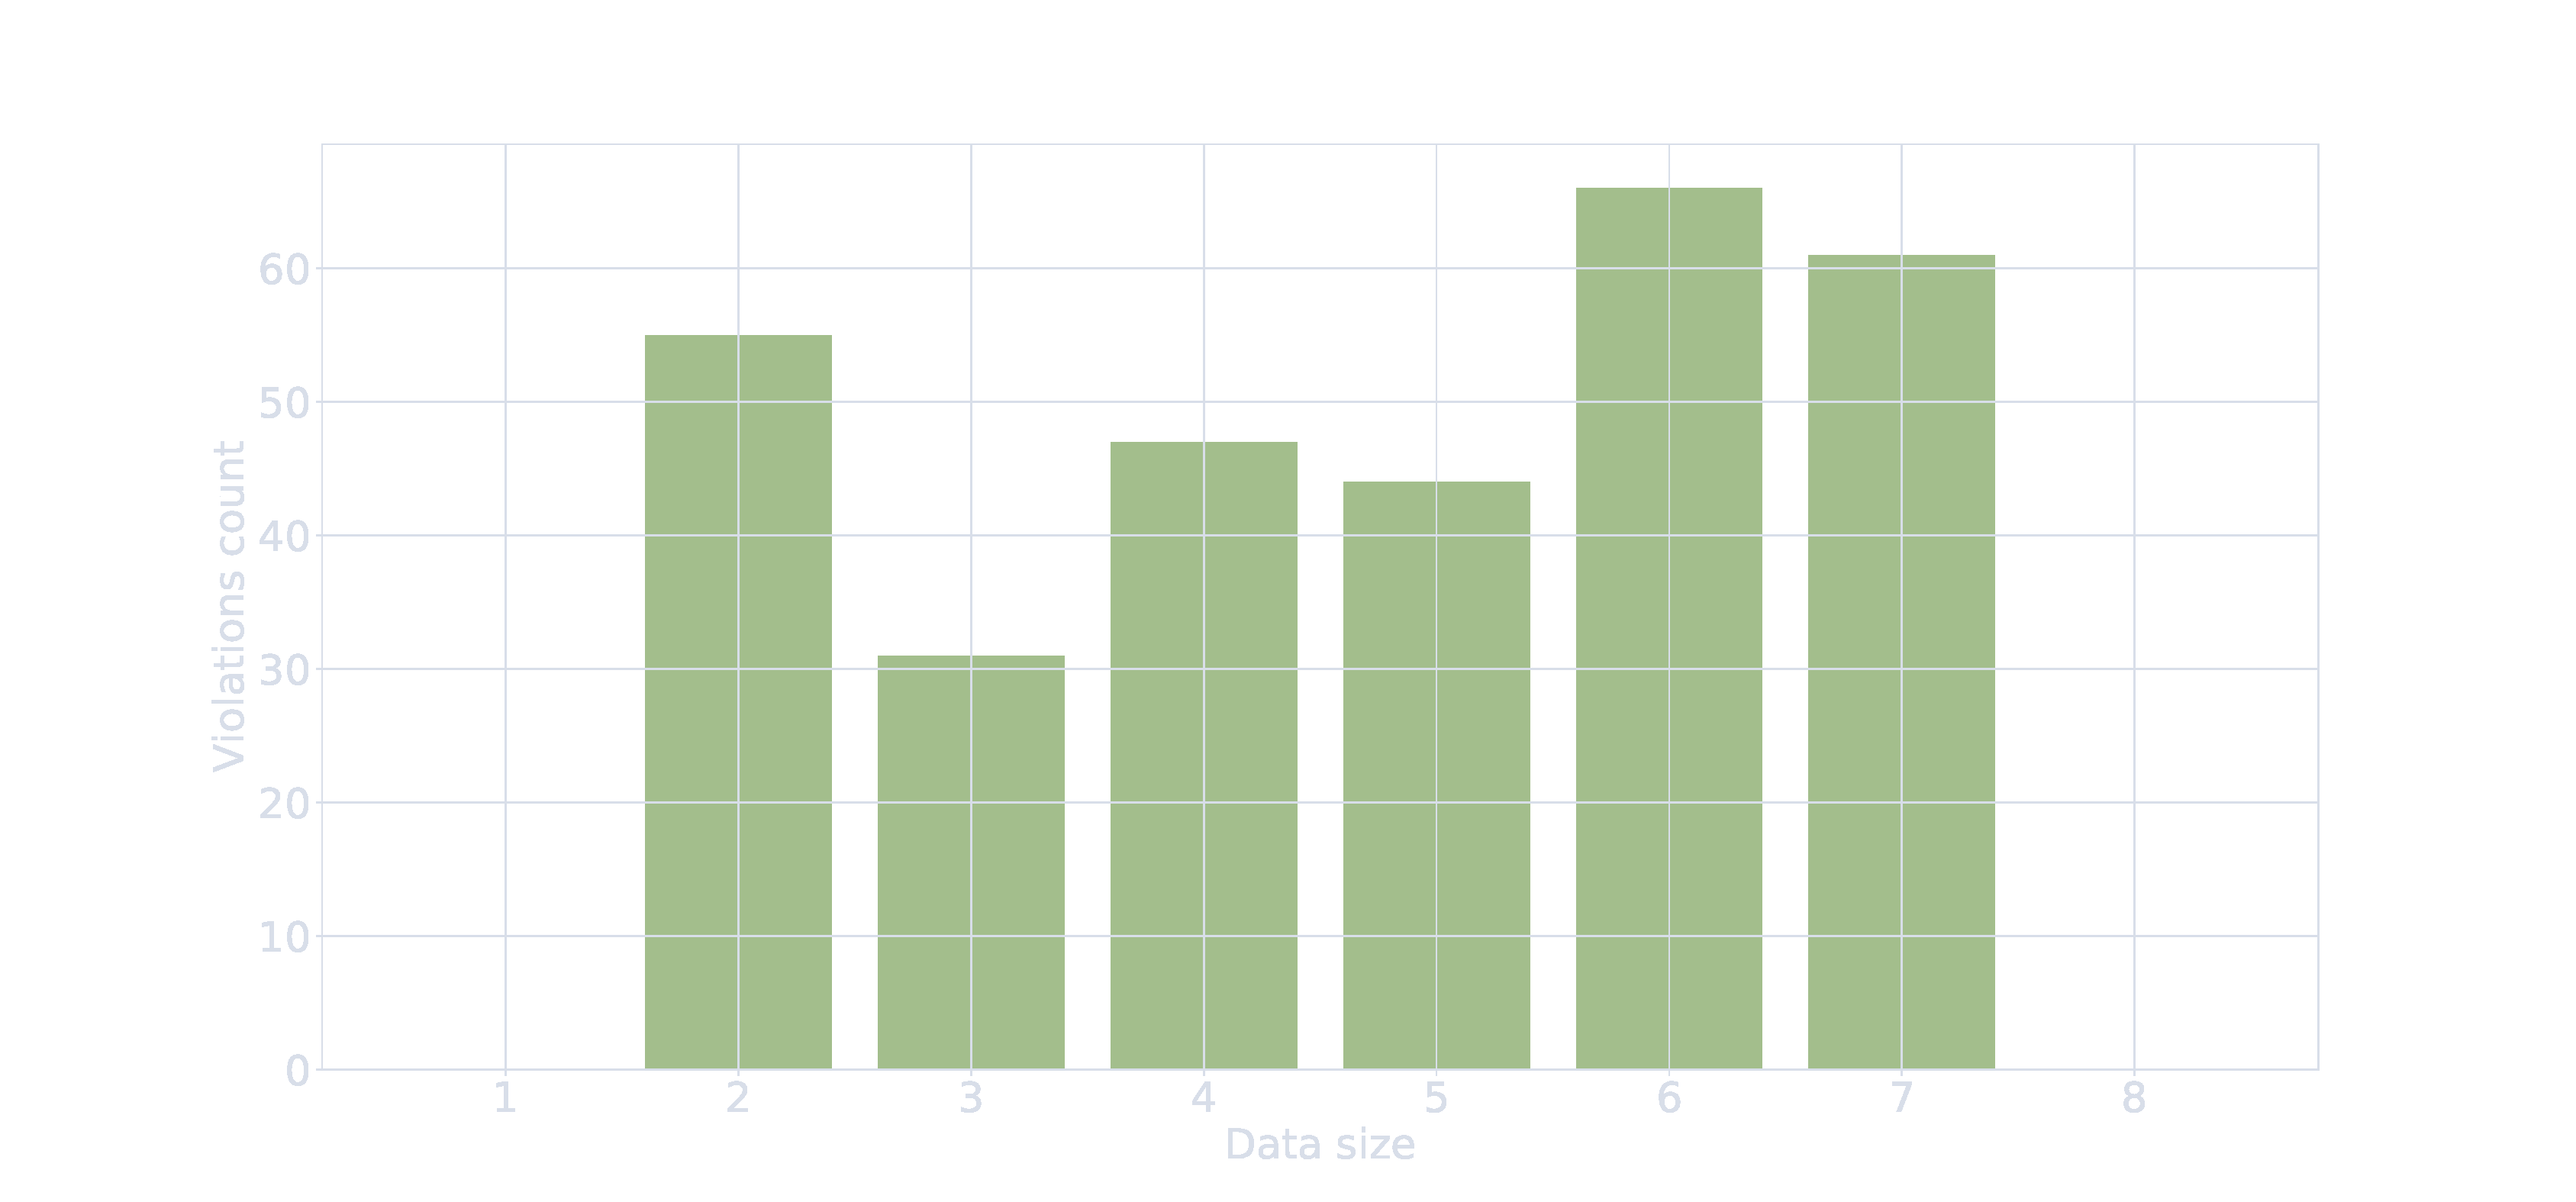
\includegraphics[width=\textwidth]{mp_violations_hist.pdf}
	\end{figure}
\end{frame}

\begin{frame}[fragile]{Message Passing}{final fix}
\centering
\begin{lstlisting}
__global__ void kernel (
    int n, volatile int * flag, int * data, int *result) { 
\end{lstlisting}

\begin{columns}[T]
	\begin{column}{0.45\textwidth}
\begin{lstlisting}[title={Writer}]
for (int i = 0; i < n; i++)
  data[i] = i + 1;
__threadfence ();

*flag = 1;
\end{lstlisting}
\end{column}

\begin{column}{0.45\textwidth}
\begin{lstlisting}[title={Reader}]
while (*flag == 0);
__threadfence ();

for (int i = 0; i < n; i++)
  if (data[i] == 0)
    *result = 0;
\end{lstlisting}
			\end{column}
	\end{columns}
\end{frame}

\begin{frame}[fragile]{Message Passing}{}
\centering
	\begin{figure}
		
\includegraphics[trim=0 20 0 0,clip,height=0.9\textheight,keepaspectratio]{threadfence_meme.jpg}
	\end{figure}
\end{frame}

\begin{frame}[fragile]{Message Passing}{Controversial version}
\centering
\begin{lstlisting}[showstringspaces=false]
__device__ int ldg (const int * p)
{
  int out;
  asm volatile("ld.global.cg.s32 %0, [%1];" : "=r"(out) : "l"(p));
  return out;
}
\end{lstlisting}

\begin{columns}[T]
	\begin{column}{0.45\textwidth}
\begin{lstlisting}[title={Writer}]
for (int i = 0; i < n; i++)
  data[i] = i + 1;
__threadfence ();

*flag = 1;
\end{lstlisting}
\end{column}

\begin{column}{0.45\textwidth}
\begin{lstlisting}[title={Reader}]
while (*flag == 0);
// __threadfence ();

for (int i = 0; i < n; i++)
  if (ldg (data + i) == 0)
    *result = 0;
\end{lstlisting}
			\end{column}
	\end{columns}
\end{frame}

\begin{frame}[fragile]{Message Passing}{n=1}
\centering
Average speedup is about $8.4\%$.

\centering
	\begin{figure}
		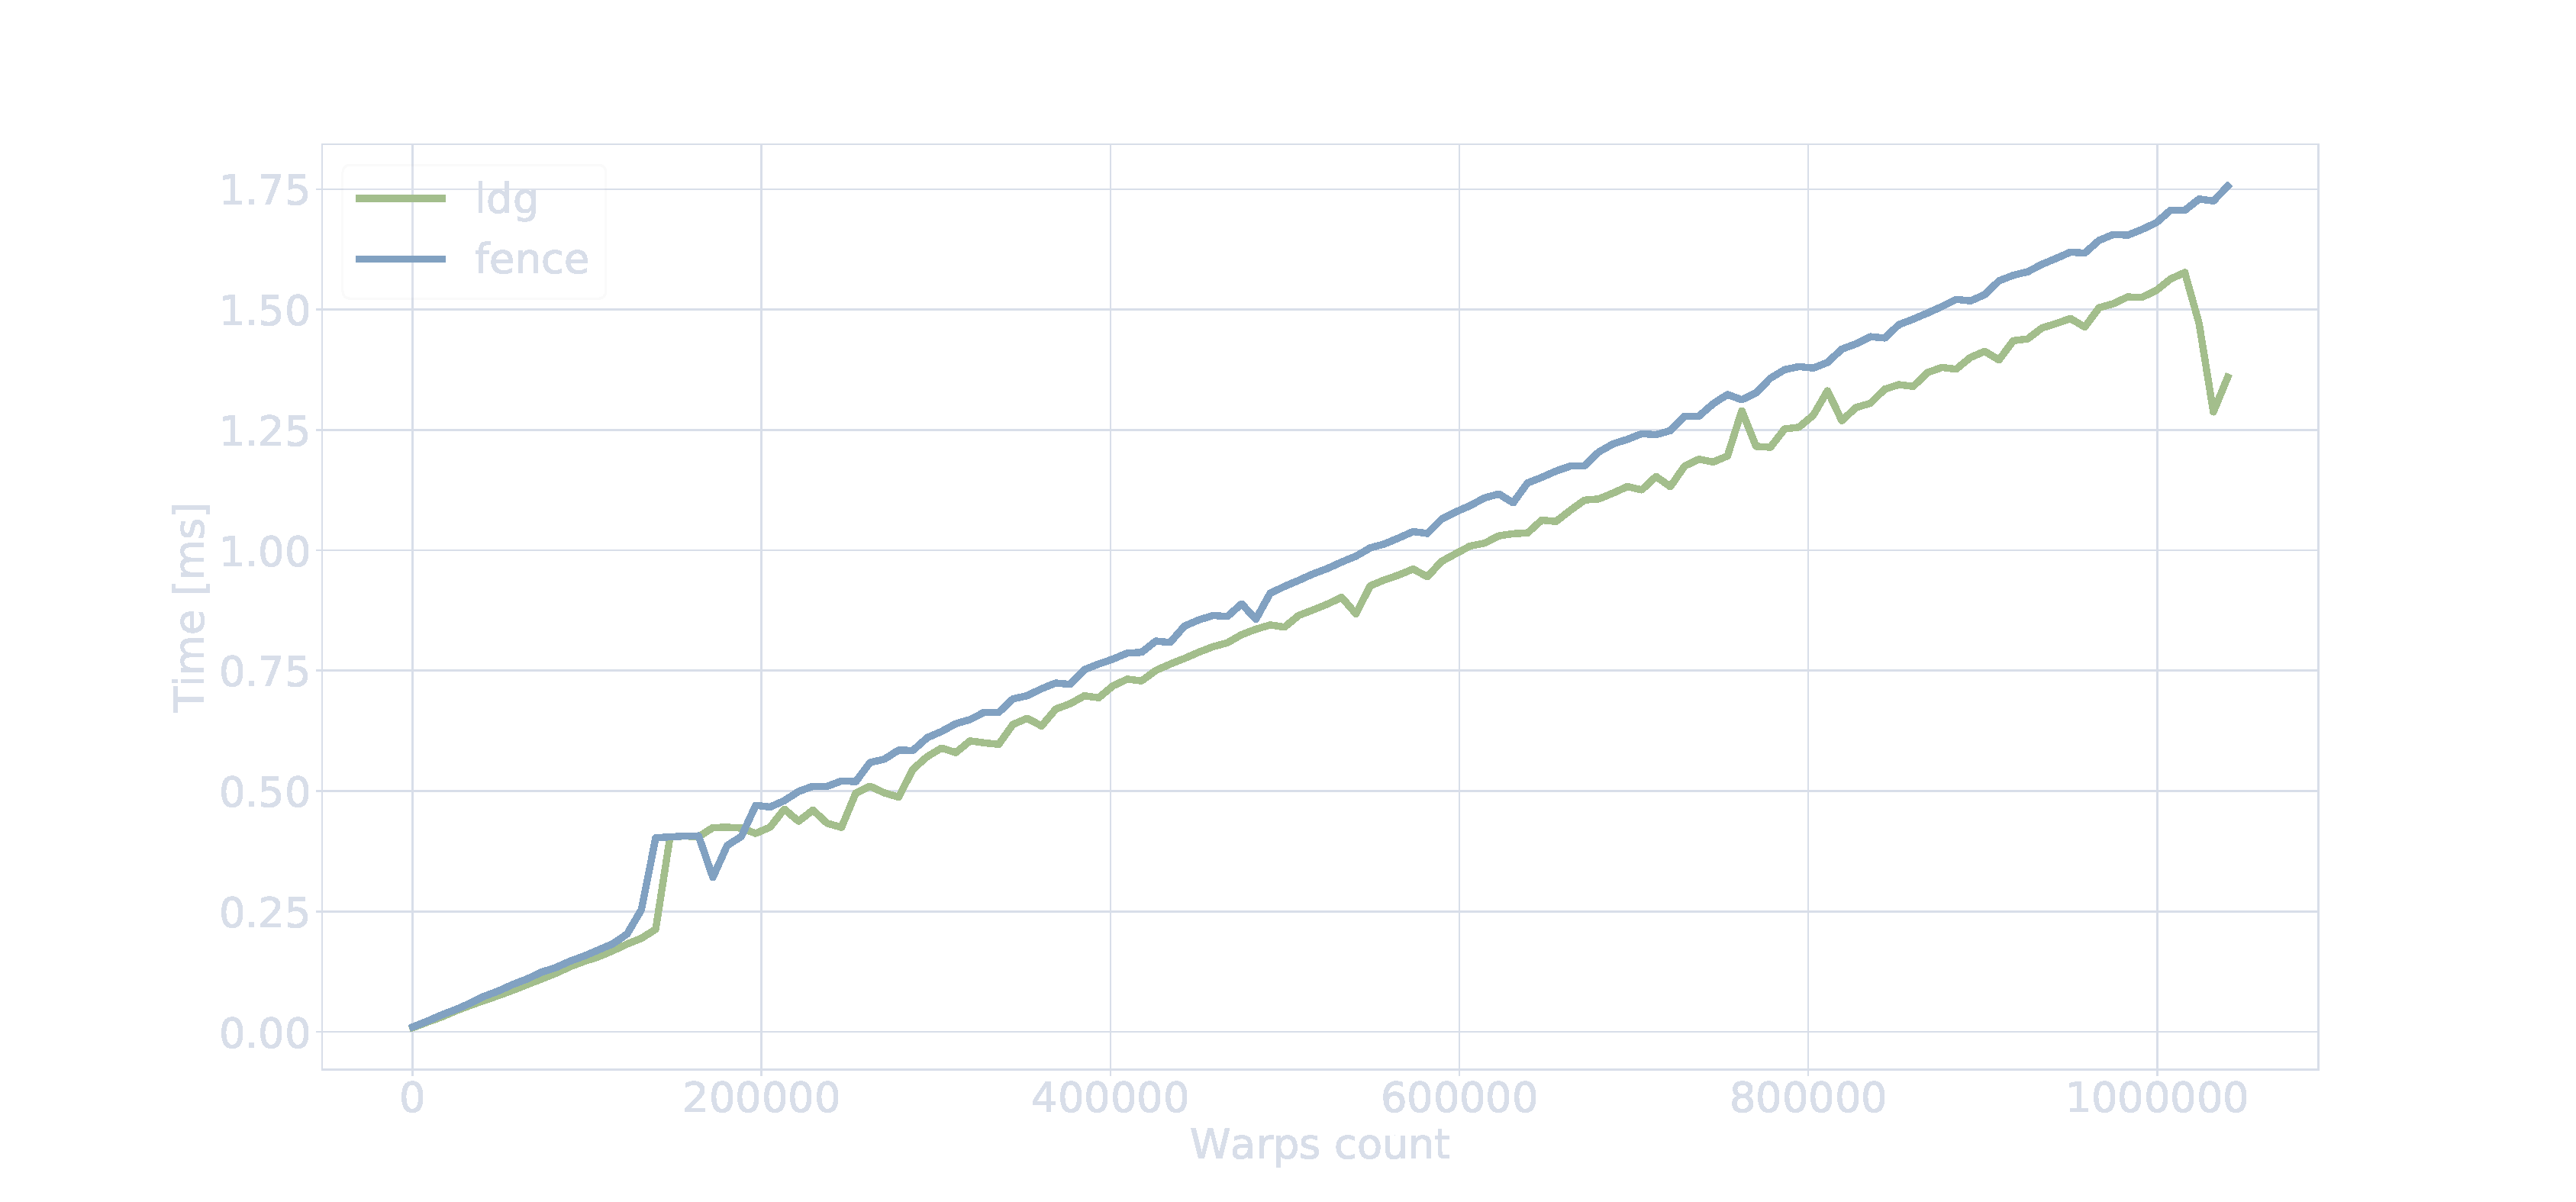
\includegraphics[width=\textwidth]{n1.pdf}
	\end{figure}
\end{frame}

\begin{frame}[fragile]{Message Passing}{}
``It’s possible to break the dependency order between the flag load and the later, dependent ld.cg load, 
that makes your test pass. Because it’s possible to write a program that breaks this order, 
it’s not possible for us to write a memory model that says the order is enforced.'' \footfullcite{Olivier}
\end{frame}

\begin{frame}[fragile]{Message Passing}{n=9}
\centering
Average slowdown is about $208.3\%$.

\centering
	\begin{figure}
		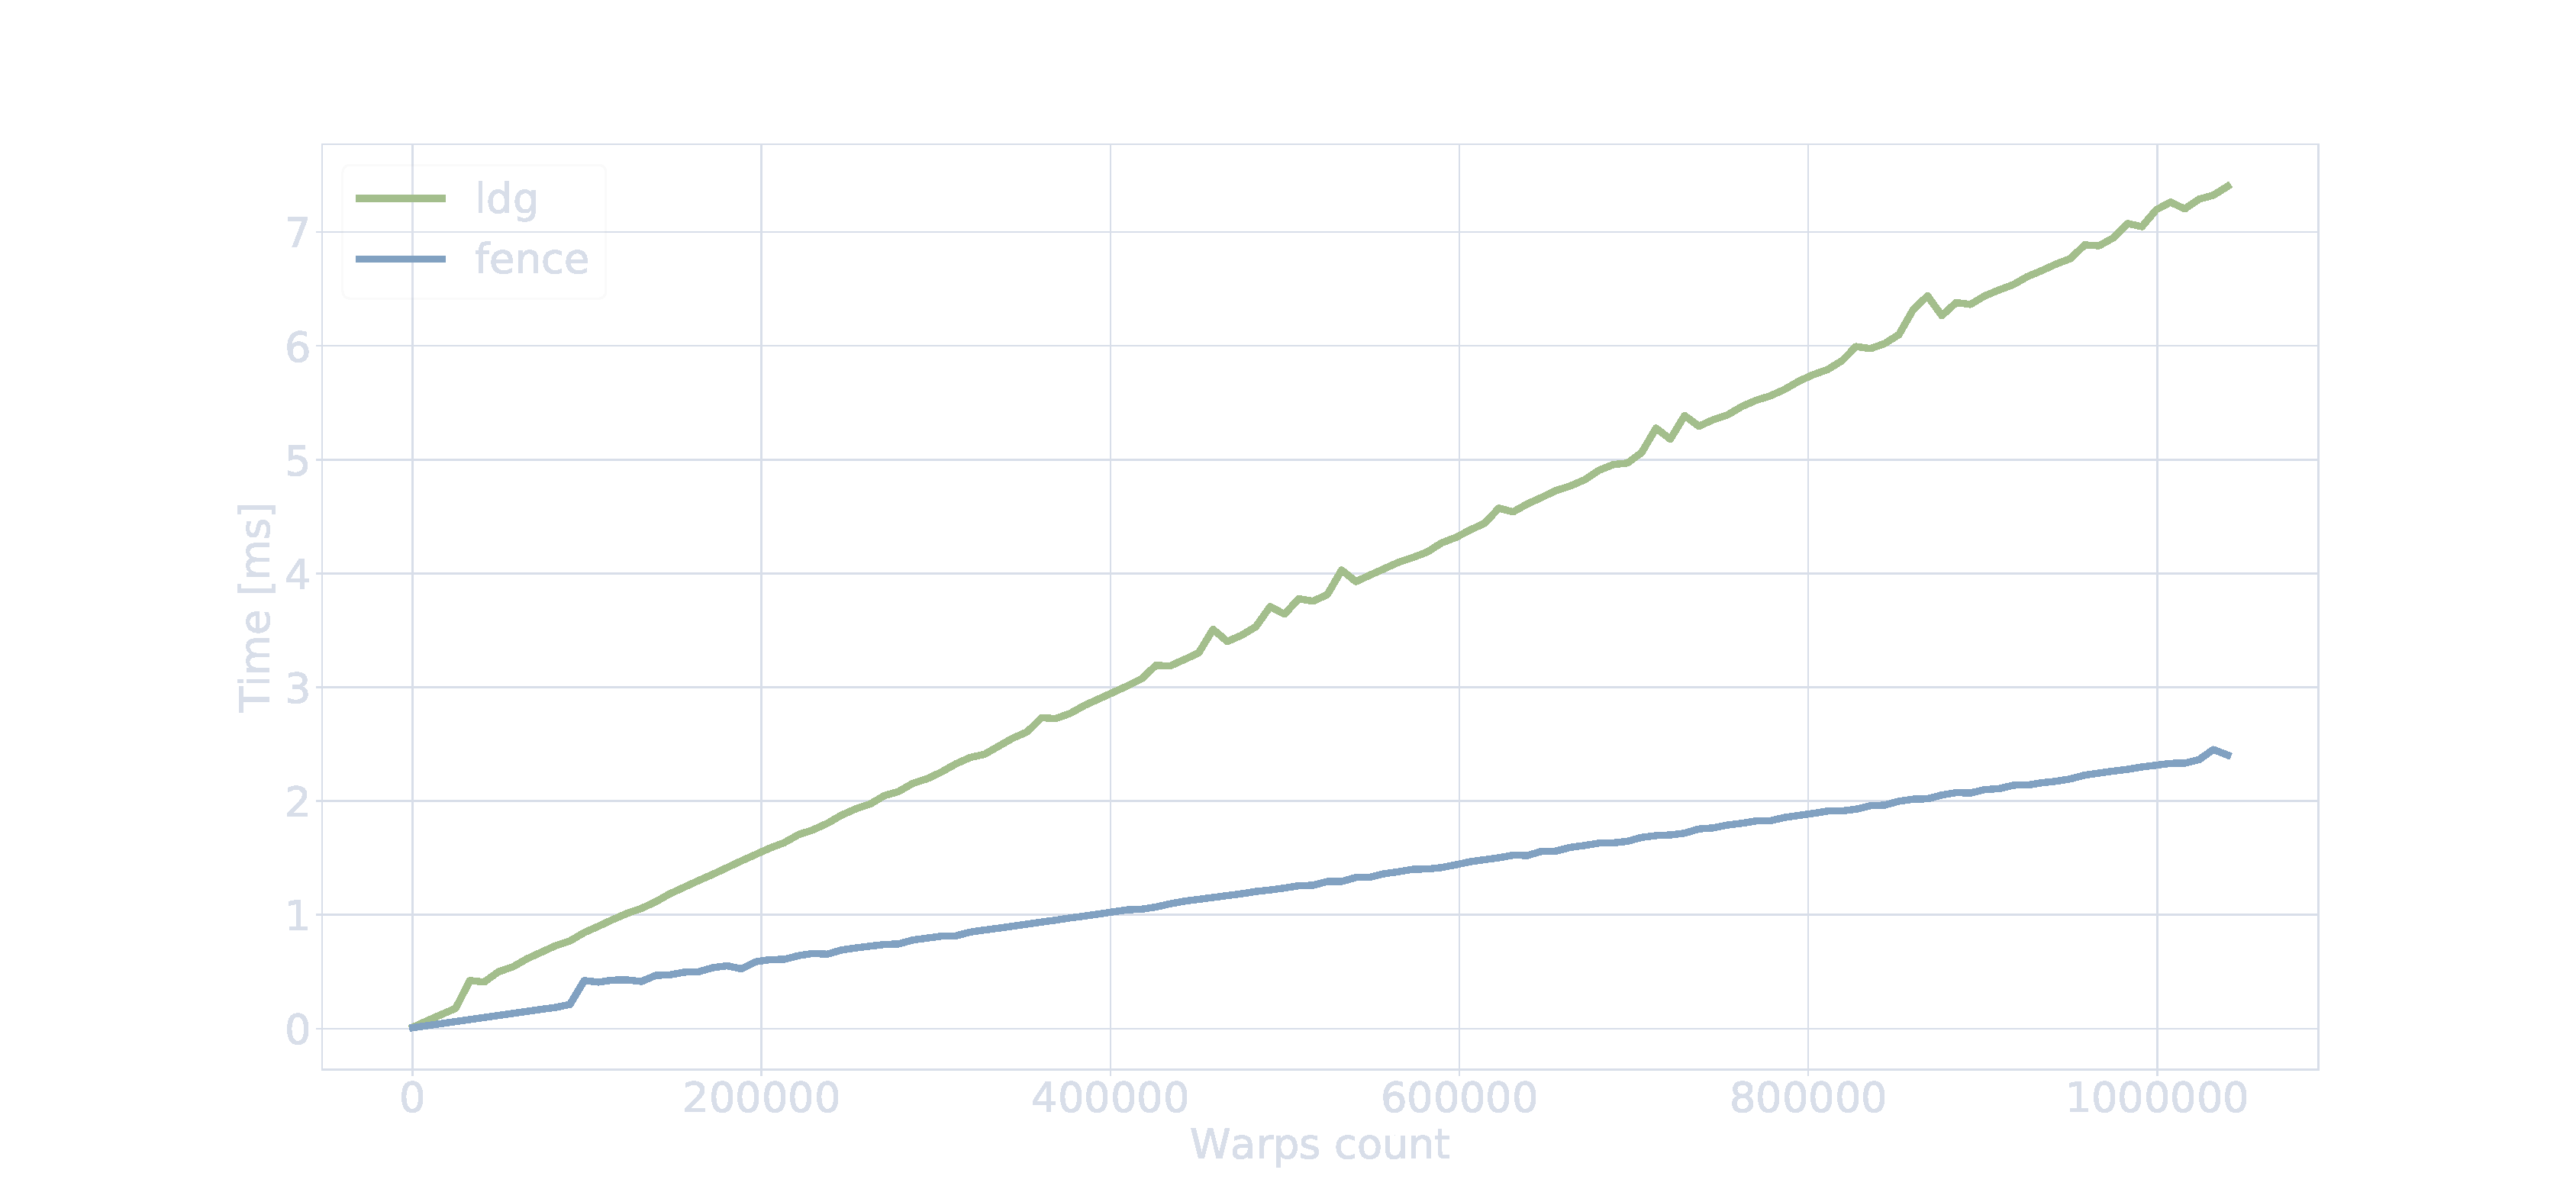
\includegraphics[width=\textwidth]{n9.pdf}
	\end{figure}
\end{frame}

\begin{frame}[fragile]{Message Passing}{}
The fence can be eliminated if the status flag and the corresponding value being updated can 
be combined into a single architectural word. \footfullcite{DecLoop}
\end{frame}

\begin{frame}[fragile]{Message Passing}{Single word}
\centering
\begin{lstlisting}[showstringspaces=false]
union data_flag
{
  struct { int32_t data; int32_t flag; } fields;
  int64_t vec;
};
\end{lstlisting}

\begin{columns}[T]
	\begin{column}{0.45\textwidth}
\begin{lstlisting}[title={Writer}]
data_flag tmp;
tmp.fields.data = 1;
tmp.fields.flag = 1;

df->vec = tmp.vec;
\end{lstlisting}
\end{column}

\begin{column}{0.45\textwidth}
\begin{lstlisting}[title={Reader}]
while (!tmp.fields.flag)
  tmp.vec = df->vec;

if (tmp.fields.data == 0)
  *result = 0;

\end{lstlisting}
			\end{column}
	\end{columns}
\end{frame}

\begin{frame}[fragile]{Message Passing}{Single word}
\centering
	\begin{figure}
		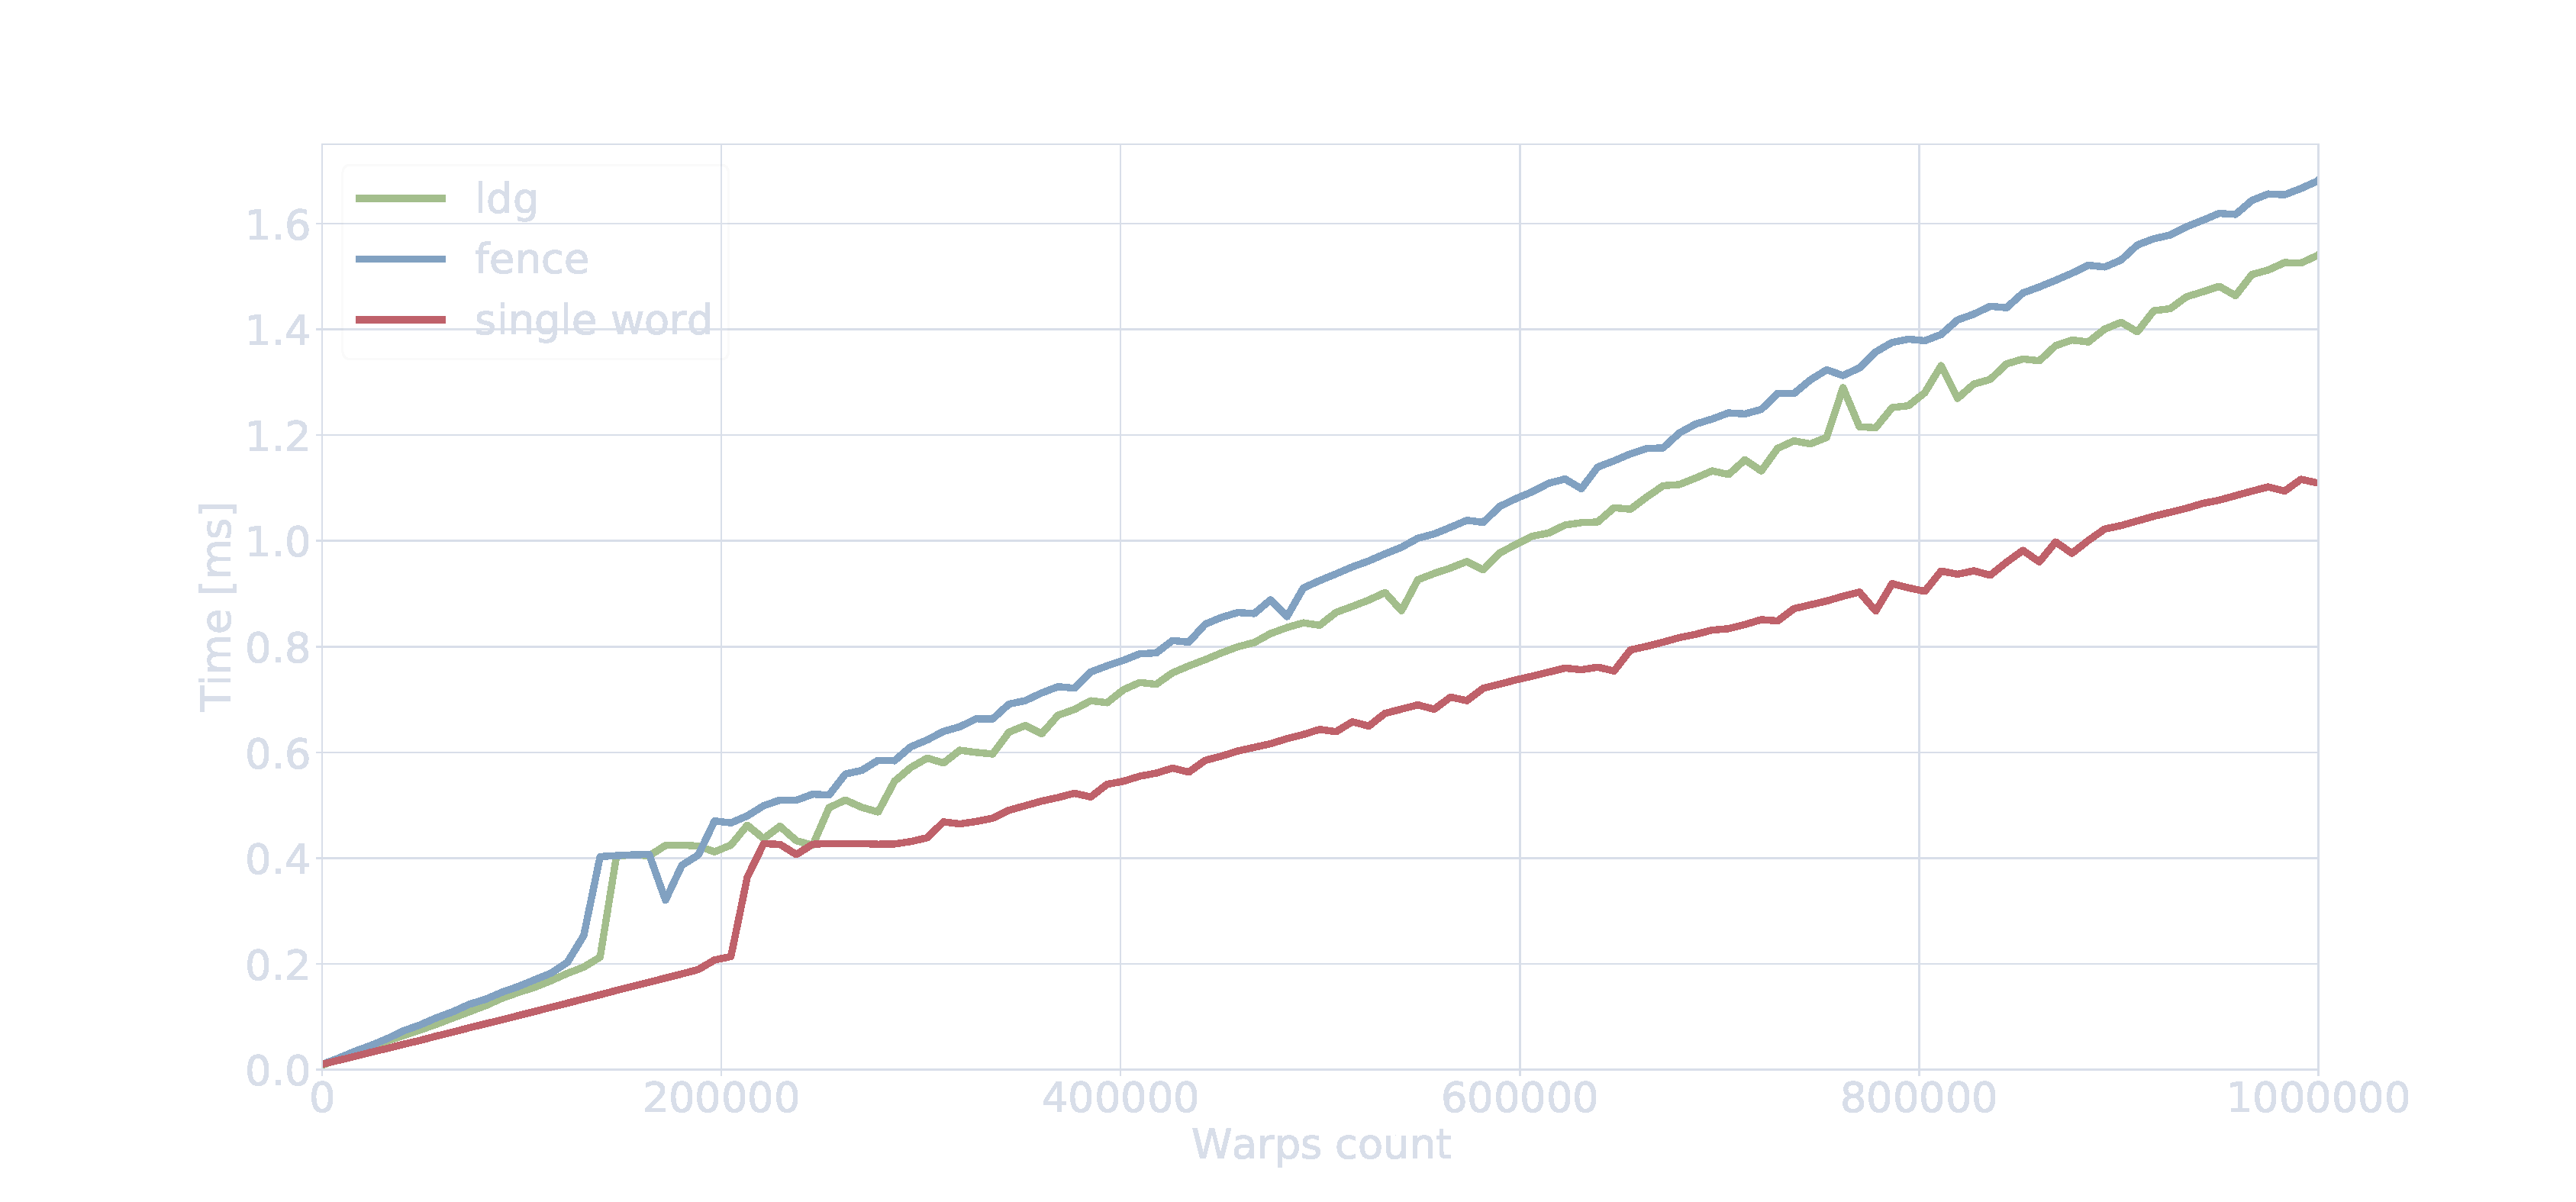
\includegraphics[width=\textwidth]{single_word.pdf}
	\end{figure}
\end{frame}


\begin{frame}[fragile]{Exclusive scan}{sequential version}

\vspace{0.1in}
Scan produces an output sequence where each element is computed to be the reduction of the elements occurring earlier in the input sequence.
\vspace{0.3in}

\begin{columns}[T]
	\begin{column}{0.35\textwidth}
\begin{lstlisting}[showstringspaces=false]
int sum = 0;
for (int i = 0; i < n; i++)
  {
    out[i] = sum;
    sum += in[i];
  }
\end{lstlisting}
	\end{column}
	\begin{column}{0.4\textwidth}
		\begin{tikzpicture}[square/.style={regular polygon,regular polygon sides=4}]
			\node[text=NordWhite] (in0) {in};
		  \foreach[count=\i] \invalue in {1,0,1,1,0,1} {
			  \pgfmathsetmacro\prev{int(\i - 1)}
				\node[fill=NordBlue, text=NordDarkBlack, right of=in\prev,square] (in\i) {\invalue};
			}
			\node[text=NordWhite,below of=in0] (out0) {out};
		  \foreach[count=\i] \invalue in {0,1,1,2,3,3} {
			  \pgfmathsetmacro\prev{int(\i - 1)}
				\node[fill=NordGreen, text=NordDarkBlack, right of=out\prev,square] (out\i) {\invalue};
			}
		\end{tikzpicture}
	\end{column}
\end{columns}
\end{frame}

\begin{frame}[c,fragile]{Exclusive scan}{inner scan}
\vspace{0.1in}
\begin{figure}
\centering
\begin{tikzpicture}[square/.style={regular polygon,regular polygon sides=4}]
	\node[text=NordWhite] (in0) {in};
	\foreach[count=\i] \invalue in {1,0,1,1,0,1} {
		\pgfmathsetmacro\prev{int(\i - 1)}
		\node[fill=NordBlue, text=NordDarkBlack, right of=in\prev,square] (in\i) {\invalue};
	}

	\node[text=NordWhite,below of=in0] (bs0) {bs};
	\foreach[count=\i] \invalue in {0,1,0,1,0,0} {
		\pgfmathsetmacro\prev{int(\i - 1)}
		\node[fill=NordGreen!65, text=NordDarkBlack, right of=bs\prev,square] (bs\i) {\invalue};
	}

	\node[below of=bs0] (stmp0) {};
	\node[below of=bs2,text=NordBlack,square] (stmp2) {1};
	\node[below of=bs4,text=NordBlack,square] (stmp4) {2};
	\node[below of=bs6,text=NordBlack,square] (stmp6) {1};

	\node[below of=stmp0] (tmp0) {};
	\node[below of=stmp2,text=NordBlack,square] (tmp2) {1};
	\node[below of=stmp4,text=NordBlack,square] (tmp4) {3};
	\node[below of=stmp6,text=NordBlack,square] (tmp6) {4};

	\node[text=NordBlack,below of=tmp0] (out0) {out};
	\foreach[count=\i] \invalue in {0,1,1,2,3,3} {
		\pgfmathsetmacro\prev{int(\i - 1)}
		\node[text=NordBlack, right of=out\prev,square] (out\i) {\invalue};
	}

  \draw[NordWhite] ($(in2)!0.5!(in3)$) -- ($(out2)!0.5!(out3)$);
  \draw[NordWhite] ($(in4)!0.5!(in5)$) -- ($(out4)!0.5!(out5)$);
\end{tikzpicture}
\end{figure}
\end{frame}

\begin{frame}[c,fragile]{Exclusive scan}{blocks' results}
\vspace{0.1in}
\begin{figure}
\centering
\begin{tikzpicture}[square/.style={regular polygon,regular polygon sides=4}]
	\node[text=NordWhite] (in0) {in};
	\foreach[count=\i] \invalue in {1,0,1,1,0,1} {
		\pgfmathsetmacro\prev{int(\i - 1)}
		\node[fill=NordBlue, text=NordDarkBlack, right of=in\prev,square] (in\i) {\invalue};
	}

	\node[text=NordWhite,below of=in0] (bs0) {bs};
	\foreach[count=\i] \invalue in {0,1,0,1,0,0} {
		\pgfmathsetmacro\prev{int(\i - 1)}
		\node[fill=NordGreen!65, text=NordDarkBlack, right of=bs\prev,square] (bs\i) {\invalue};
	}

	\node[below of=bs0] (stmp0) {};
	\node[below of=bs2,square,fill=NordYellow, text=NordDarkBlack] (stmp2) {1};
	\node[below of=bs4,square,fill=NordYellow, text=NordDarkBlack] (stmp4) {2};
	\node[below of=bs6,square,fill=NordYellow, text=NordDarkBlack] (stmp6) {1};

	\node[below of=stmp0] (tmp0) {};
	\node[below of=stmp2,text=NordBlack,square] (tmp2) {1};
	\node[below of=stmp4,text=NordBlack,square] (tmp4) {3};
	\node[below of=stmp6,text=NordBlack,square] (tmp6) {4};

	\node[text=NordBlack,below of=tmp0] (out0) {out};
	\foreach[count=\i] \invalue in {0,1,1,2,3,3} {
		\pgfmathsetmacro\prev{int(\i - 1)}
		\node[text=NordBlack, right of=out\prev,square] (out\i) {\invalue};
	}

  \draw[NordWhite] ($(in2)!0.5!(in3)$) -- ($(out2)!0.5!(out3)$);
  \draw[NordWhite] ($(in4)!0.5!(in5)$) -- ($(out4)!0.5!(out5)$);
\end{tikzpicture}
\end{figure}
\end{frame}

\begin{frame}[c,fragile]{Exclusive scan}{inclusive scan of blocks' results}
\vspace{0.1in}
\begin{figure}
\centering
\begin{tikzpicture}[square/.style={regular polygon,regular polygon sides=4}]
	\node[text=NordWhite] (in0) {in};
	\foreach[count=\i] \invalue in {1,0,1,1,0,1} {
		\pgfmathsetmacro\prev{int(\i - 1)}
		\node[fill=NordBlue, text=NordDarkBlack, right of=in\prev,square] (in\i) {\invalue};
	}

	\node[text=NordWhite,below of=in0] (bs0) {bs};
	\foreach[count=\i] \invalue in {0,1,0,1,0,0} {
		\pgfmathsetmacro\prev{int(\i - 1)}
		\node[fill=NordGreen!65, text=NordDarkBlack, right of=bs\prev,square] (bs\i) {\invalue};
	}

	\node[below of=bs0] (stmp0) {};
	\node[below of=bs2,square,fill=NordYellow, text=NordDarkBlack] (stmp2) {1};
	\node[below of=bs4,square,fill=NordYellow, text=NordDarkBlack] (stmp4) {2};
	\node[below of=bs6,square,fill=NordYellow, text=NordDarkBlack] (stmp6) {1};

	\node[below of=stmp0] (tmp0) {};
	\node[below of=stmp2,fill=NordYellow, text=NordDarkBlack,square] (tmp2) {1};
	\node[below of=stmp4,fill=NordYellow, text=NordDarkBlack,square] (tmp4) {3};
	\node[below of=stmp6,fill=NordYellow, text=NordDarkBlack,square] (tmp6) {4};

	\node[text=NordBlack,below of=tmp0] (out0) {out};
	\foreach[count=\i] \invalue in {0,1,1,2,3,3} {
		\pgfmathsetmacro\prev{int(\i - 1)}
		\node[text=NordBlack, right of=out\prev,square] (out\i) {\invalue};
	}

  \draw[NordWhite] ($(in2)!0.5!(in3)$) -- ($(out2)!0.5!(out3)$);
  \draw[NordWhite] ($(in4)!0.5!(in5)$) -- ($(out4)!0.5!(out5)$);
\end{tikzpicture}
\end{figure}
\end{frame}

\begin{frame}[c,fragile]{Exclusive scan}{final result}
\vspace{0.1in}
\begin{figure}
\centering
\begin{tikzpicture}[square/.style={regular polygon,regular polygon sides=4}]
	\node[text=NordWhite] (in0) {in};
	\foreach[count=\i] \invalue in {1,0,1,1,0,1} {
		\pgfmathsetmacro\prev{int(\i - 1)}
		\node[fill=NordBlue, text=NordDarkBlack, right of=in\prev,square] (in\i) {\invalue};
	}

	\node[text=NordWhite,below of=in0] (bs0) {bs};
	\foreach[count=\i] \invalue in {0,1,0,1,0,0} {
		\pgfmathsetmacro\prev{int(\i - 1)}
		\node[fill=NordGreen!65, text=NordDarkBlack, right of=bs\prev,square] (bs\i) {\invalue};
	}

	\node[below of=bs0] (stmp0) {};
	\node[below of=bs2,fill=NordYellow, text=NordDarkBlack,square] (stmp2) {1};
	\node[below of=bs4,fill=NordYellow, text=NordDarkBlack,square] (stmp4) {2};
	\node[below of=bs6,fill=NordYellow, text=NordDarkBlack,square] (stmp6) {1};

	\node[below of=stmp0] (tmp0) {};
	\node[below of=stmp2,fill=NordYellow, text=NordDarkBlack,square] (tmp2) {1};
	\node[below of=stmp4,fill=NordYellow, text=NordDarkBlack,square] (tmp4) {3};
	\node[below of=stmp6,fill=NordYellow, text=NordDarkBlack,square] (tmp6) {4};

	\node[text=NordWhite,below of=tmp0] (out0) {out};
	\foreach[count=\i] \invalue in {0,1,1,2,3,3} {
		\pgfmathsetmacro\prev{int(\i - 1)}
		\node[fill=NordGreen, text=NordDarkBlack, right of=out\prev,square] (out\i) {\invalue};
	}

  \draw[NordWhite] ($(in2)!0.5!(in3)$) -- ($(out2)!0.5!(out3)$);
  \draw[NordWhite] ($(in4)!0.5!(in5)$) -- ($(out4)!0.5!(out5)$);
\end{tikzpicture}
\end{figure}
\end{frame}

\begin{frame}[c,fragile]{Exclusive scan}{three-kernels version}
\begin{lstlisting}[showstringspaces=false]
hierarchical_partial_scan<<<blocks, hierarchical_block_size>>> (
  in, out, helper_buffer);

hierarchical_blocks_results_scan<<<1, 1024>>> (
  blocks, helper_buffer, helper_buffer);

hierarchical_final_adjust<<<blocks, hierarchical_block_size>>> (
  out, helper_buffer);
\end{lstlisting}
\end{frame}

\begin{frame}[fragile]{Exclusive scan}{three-kernels scan performance}
\centering
	\begin{figure}
		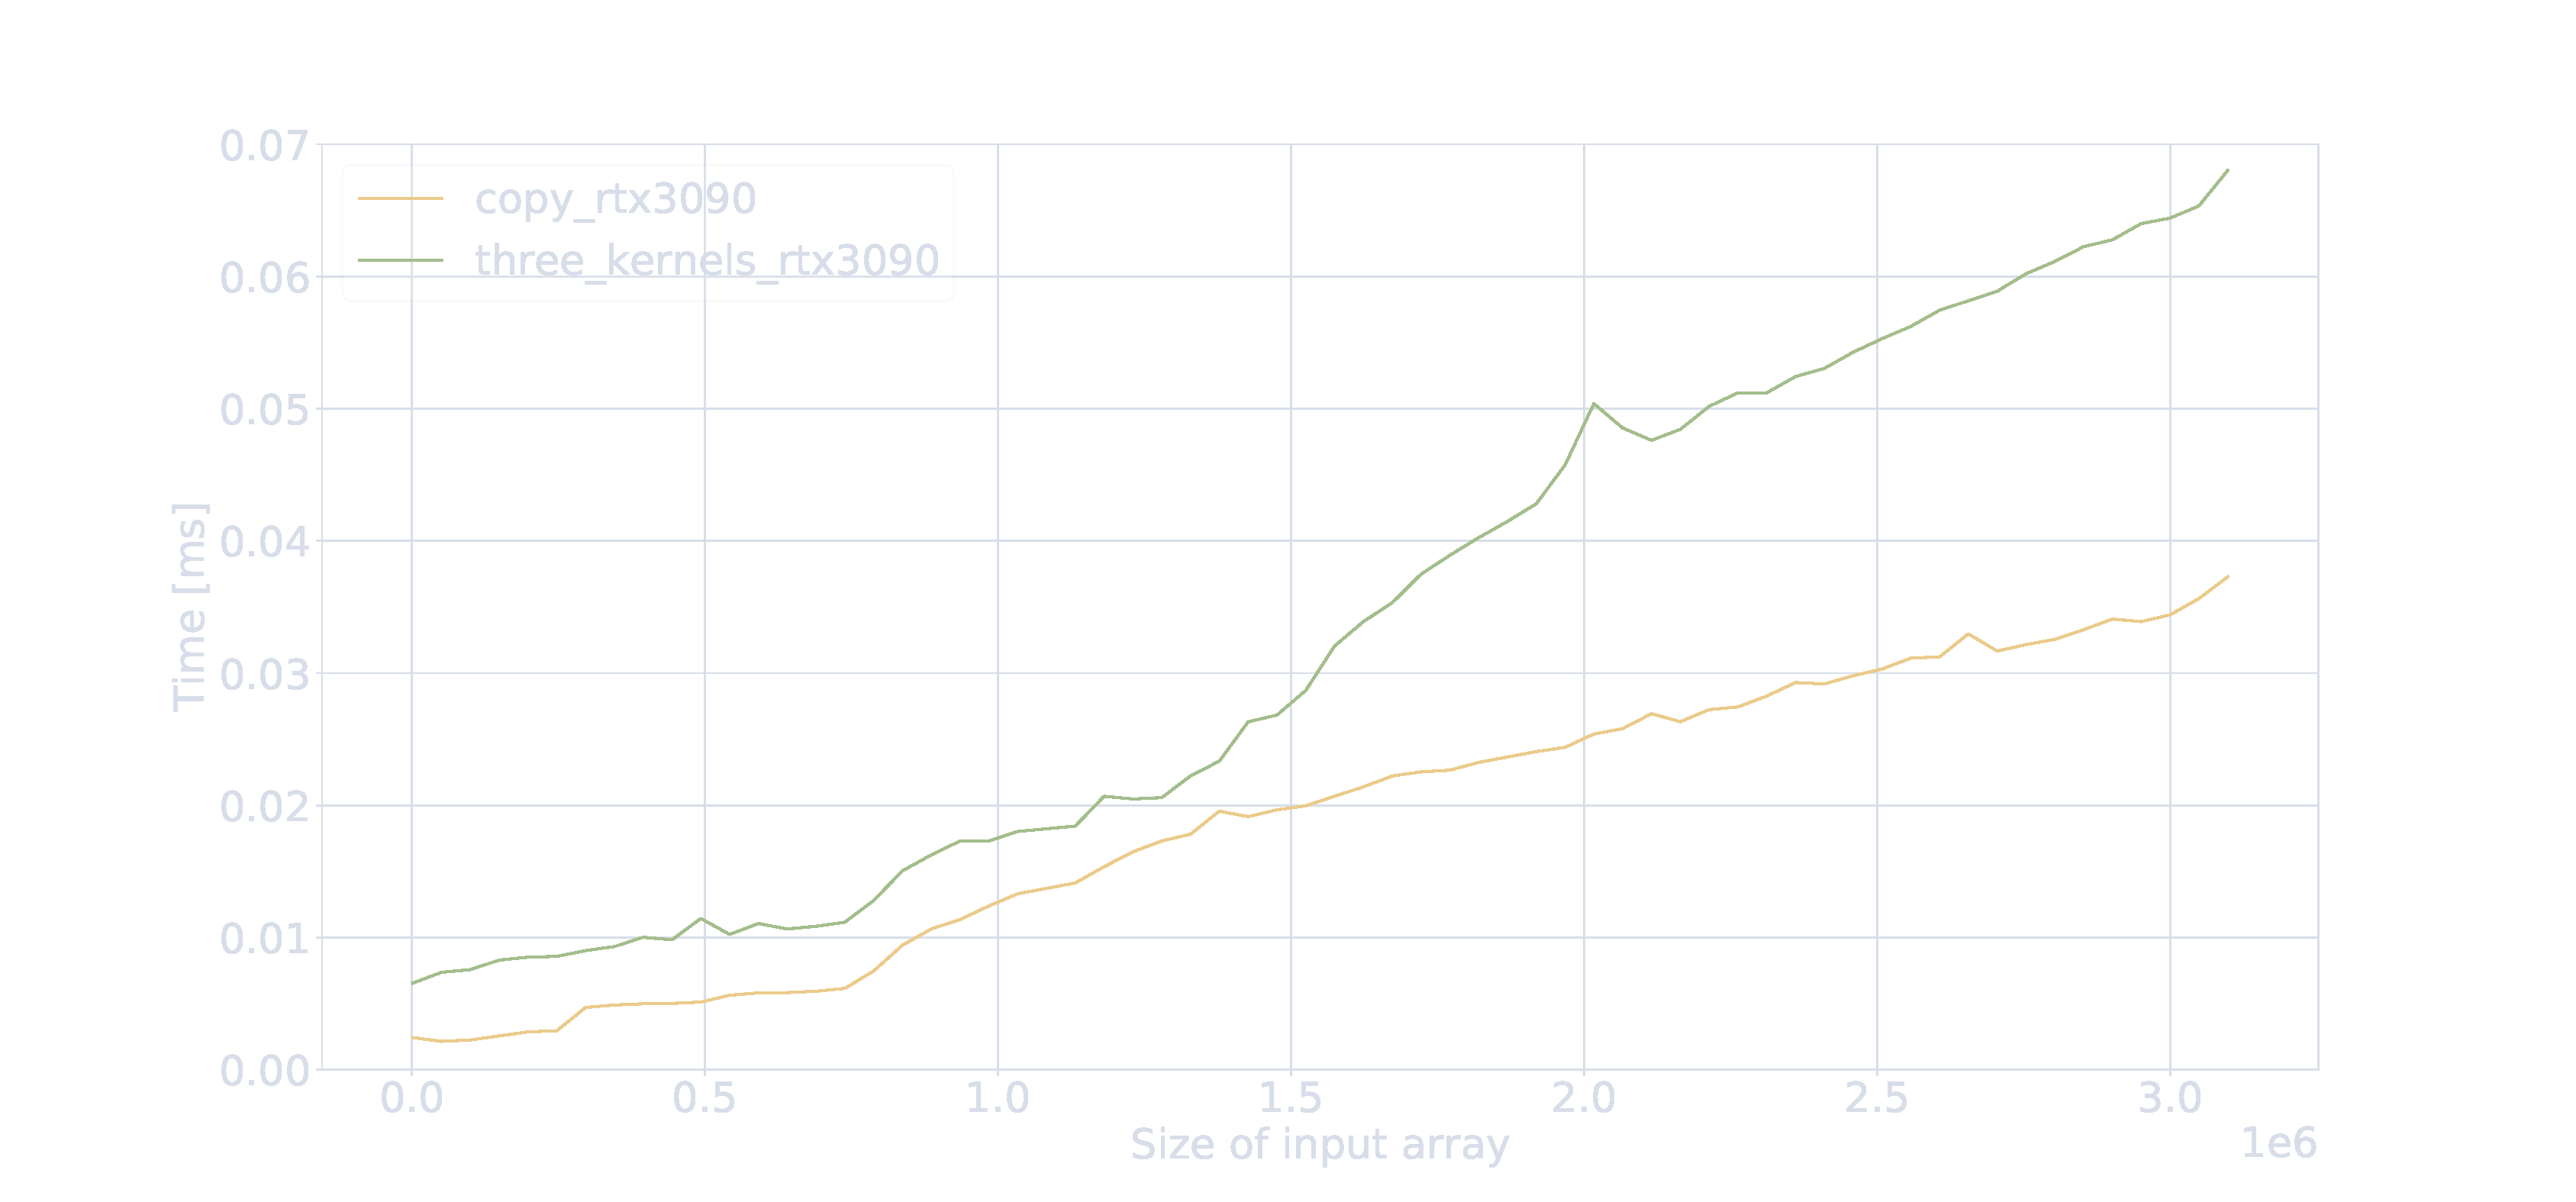
\includegraphics[width=\textwidth]{three_kernel_scan_perf.pdf}
	\end{figure}
\end{frame}

\begin{frame}[fragile]{Exclusive scan}{sequential version}

\vspace{0.1in}

\begin{lstlisting}[showstringspaces=false]
// Load 
data_type thread_data[thread_data_size];

BlockLoad (temp_storage).Load (in + block_offset, thread_data);
__syncthreads ();

// This thread block aggregate
data_type block_reduce = 
  BlockReduce (temp_storage).Sum (thread_data);

/// ...
\end{lstlisting}
\end{frame}

\begin{frame}[fragile]{Exclusive scan}{sequential version}

\vspace{0.1in}

\begin{lstlisting}[showstringspaces=false]
if (threadIdx.x == 0) {
  if (blockIdx.x == 0) {
    commit (block_statuses + blockIdx.x, block_reduce);
  }
  else {
    do {
      prev_block_status = load (block_statuses + blockIdx.x - 1);
    } while (prev_block_status.flag == 0);

    thread_data[0] += prev_block_status.data;
    commit (
      block_statuses + blockIdx.x,
      prev_block_status.data + block_reduce);
  }
}
__syncthreads ();
\end{lstlisting}
\end{frame}

\begin{frame}[fragile]{Exclusive scan}{sequential version}

\vspace{0.1in}

\begin{lstlisting}[showstringspaces=false]
BlockScan (temp_storage).ExclusiveSum (thread_data, thread_data);
__syncthreads ();

// Store final result
BlockStore (temp_storage).Store (out + block_offset, thread_data);
\end{lstlisting}
\end{frame}

\begin{frame}[fragile]{Exclusive scan}{single scan performance}
\centering
	\begin{figure}
		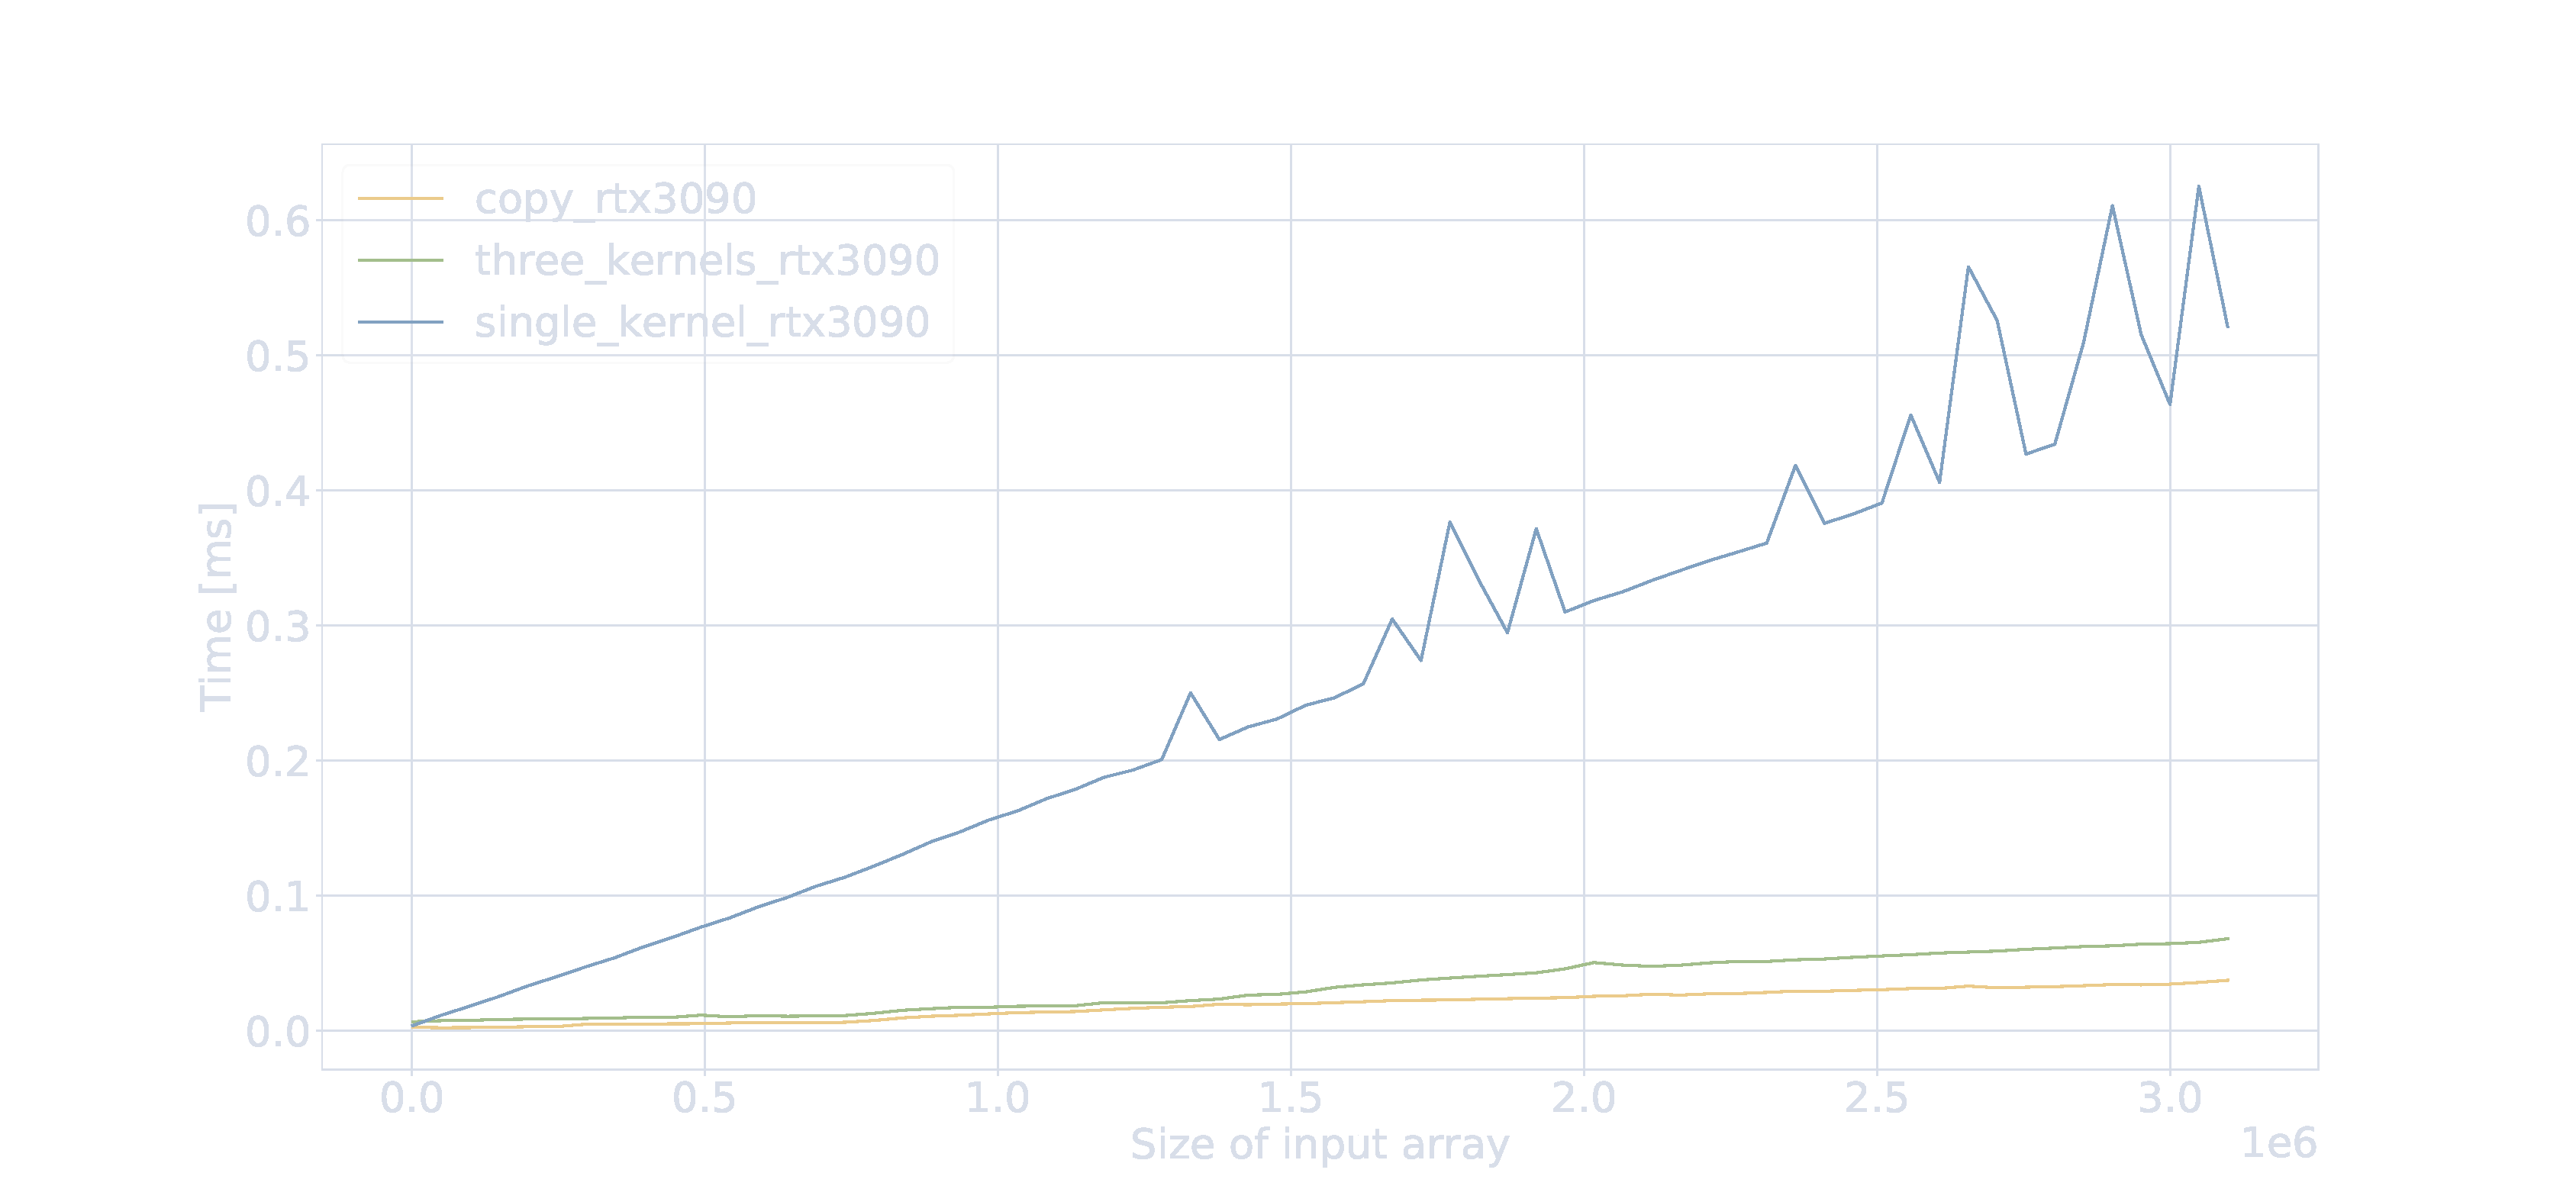
\includegraphics[width=\textwidth]{single_kernel_scan_perf.pdf}
	\end{figure}
\end{frame}

\begin{frame}[fragile]{Exclusive scan}{single scan performance}
\centering
	\begin{figure}
		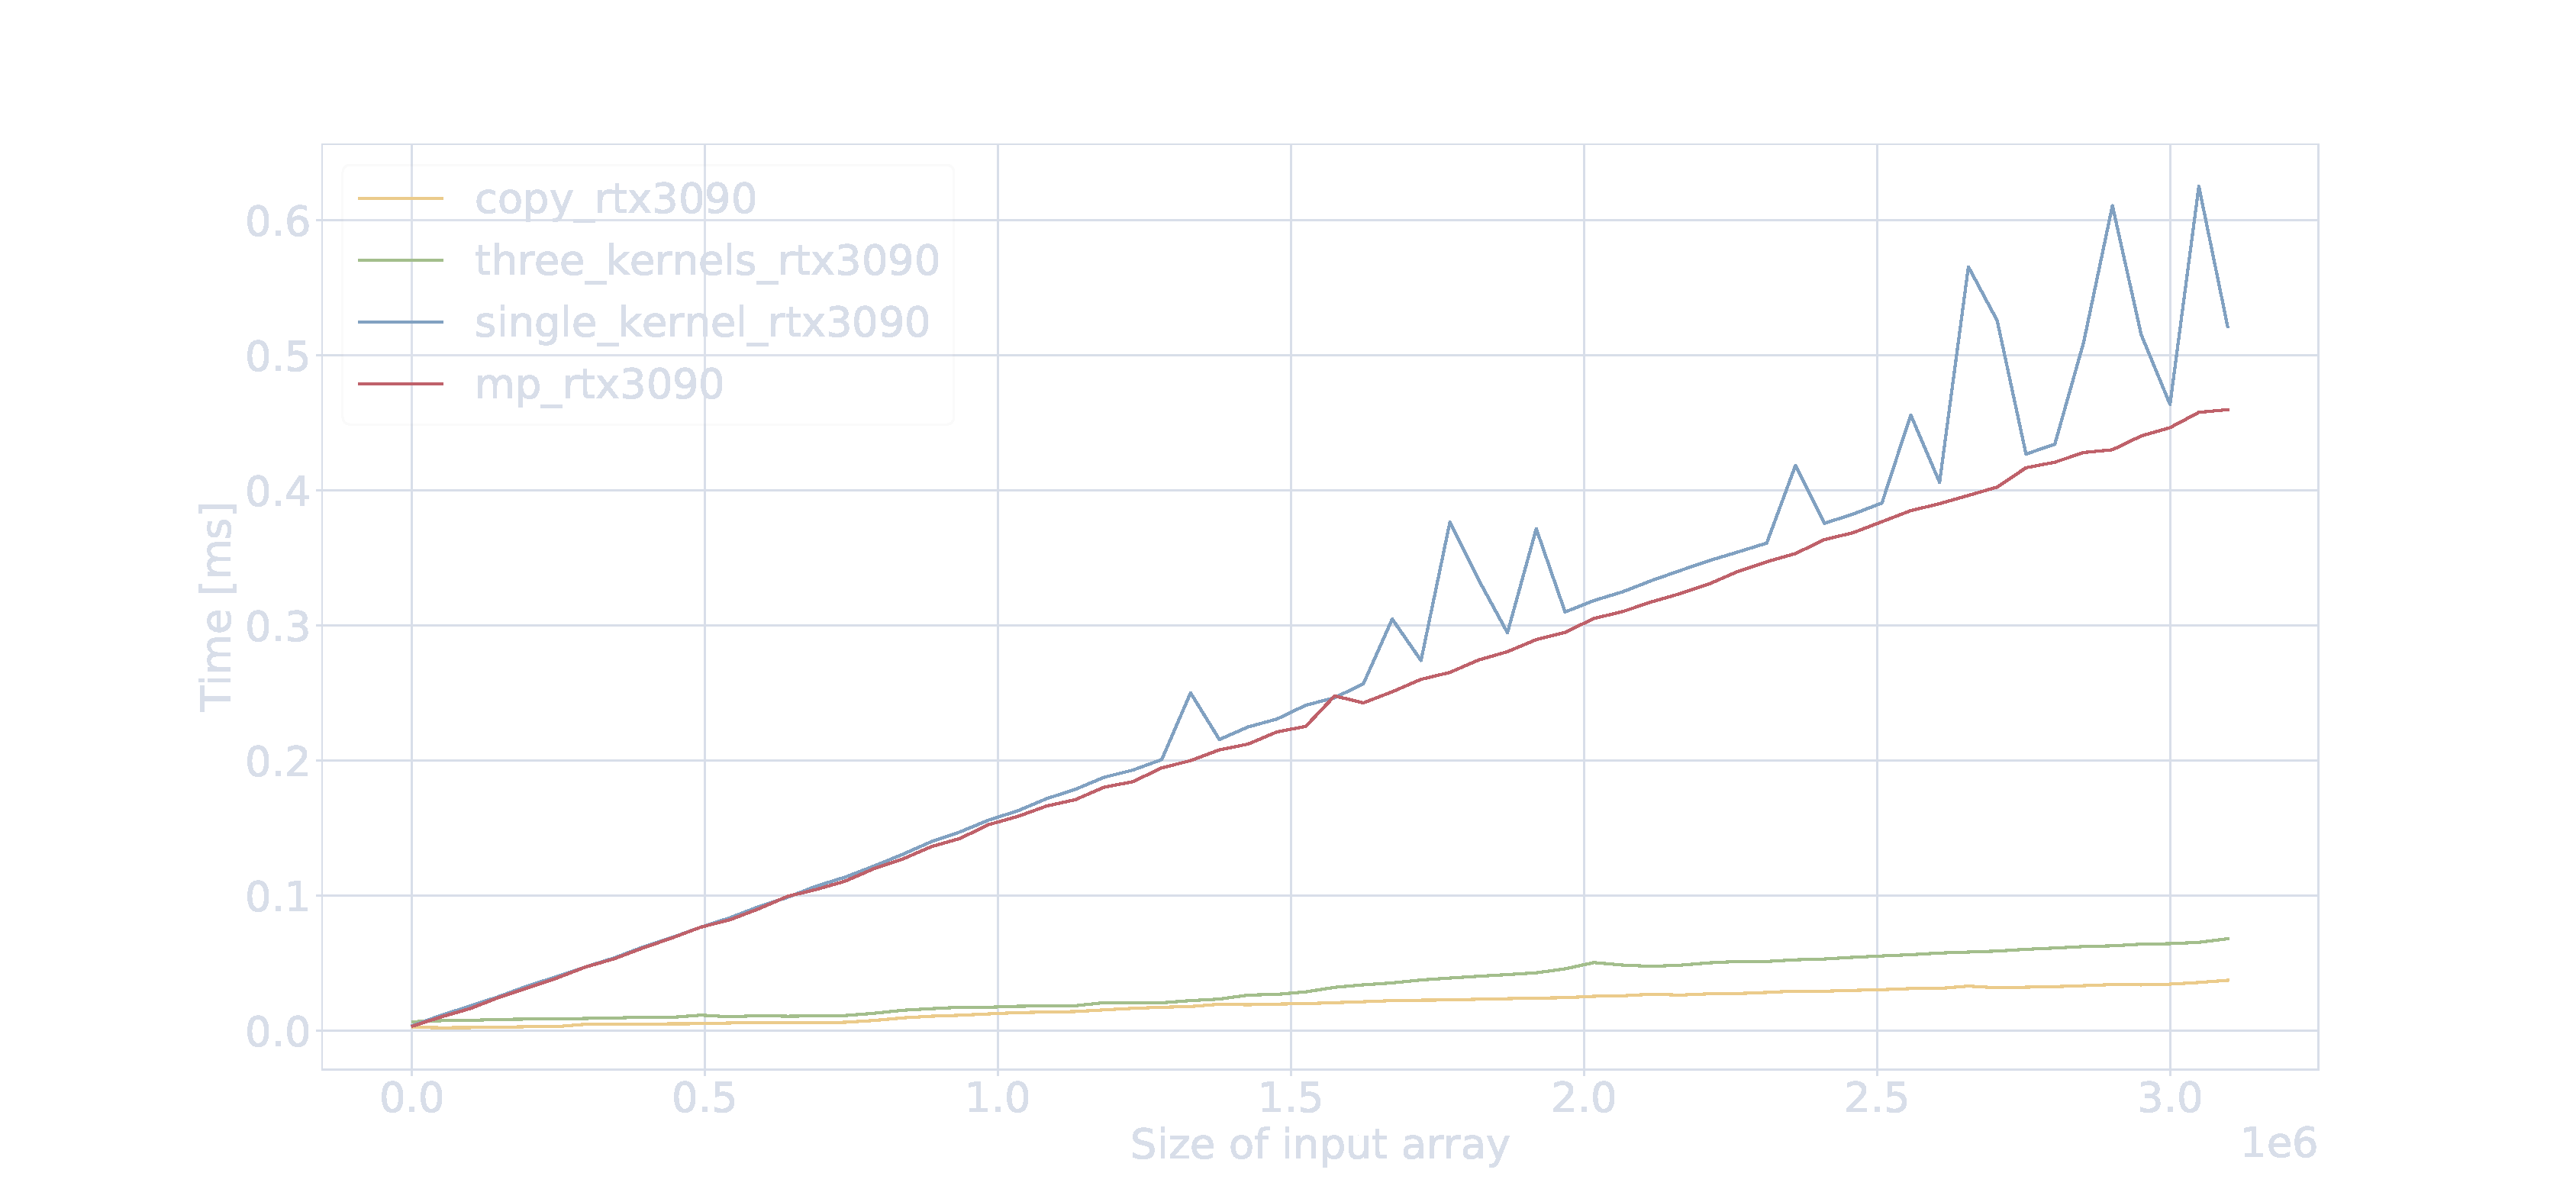
\includegraphics[width=\textwidth]{single_kernel_scan_perf_mp.pdf}
	\end{figure}
\end{frame}


\begin{frame}[fragile]{Message Passing}{}
\centering
	\begin{figure}
		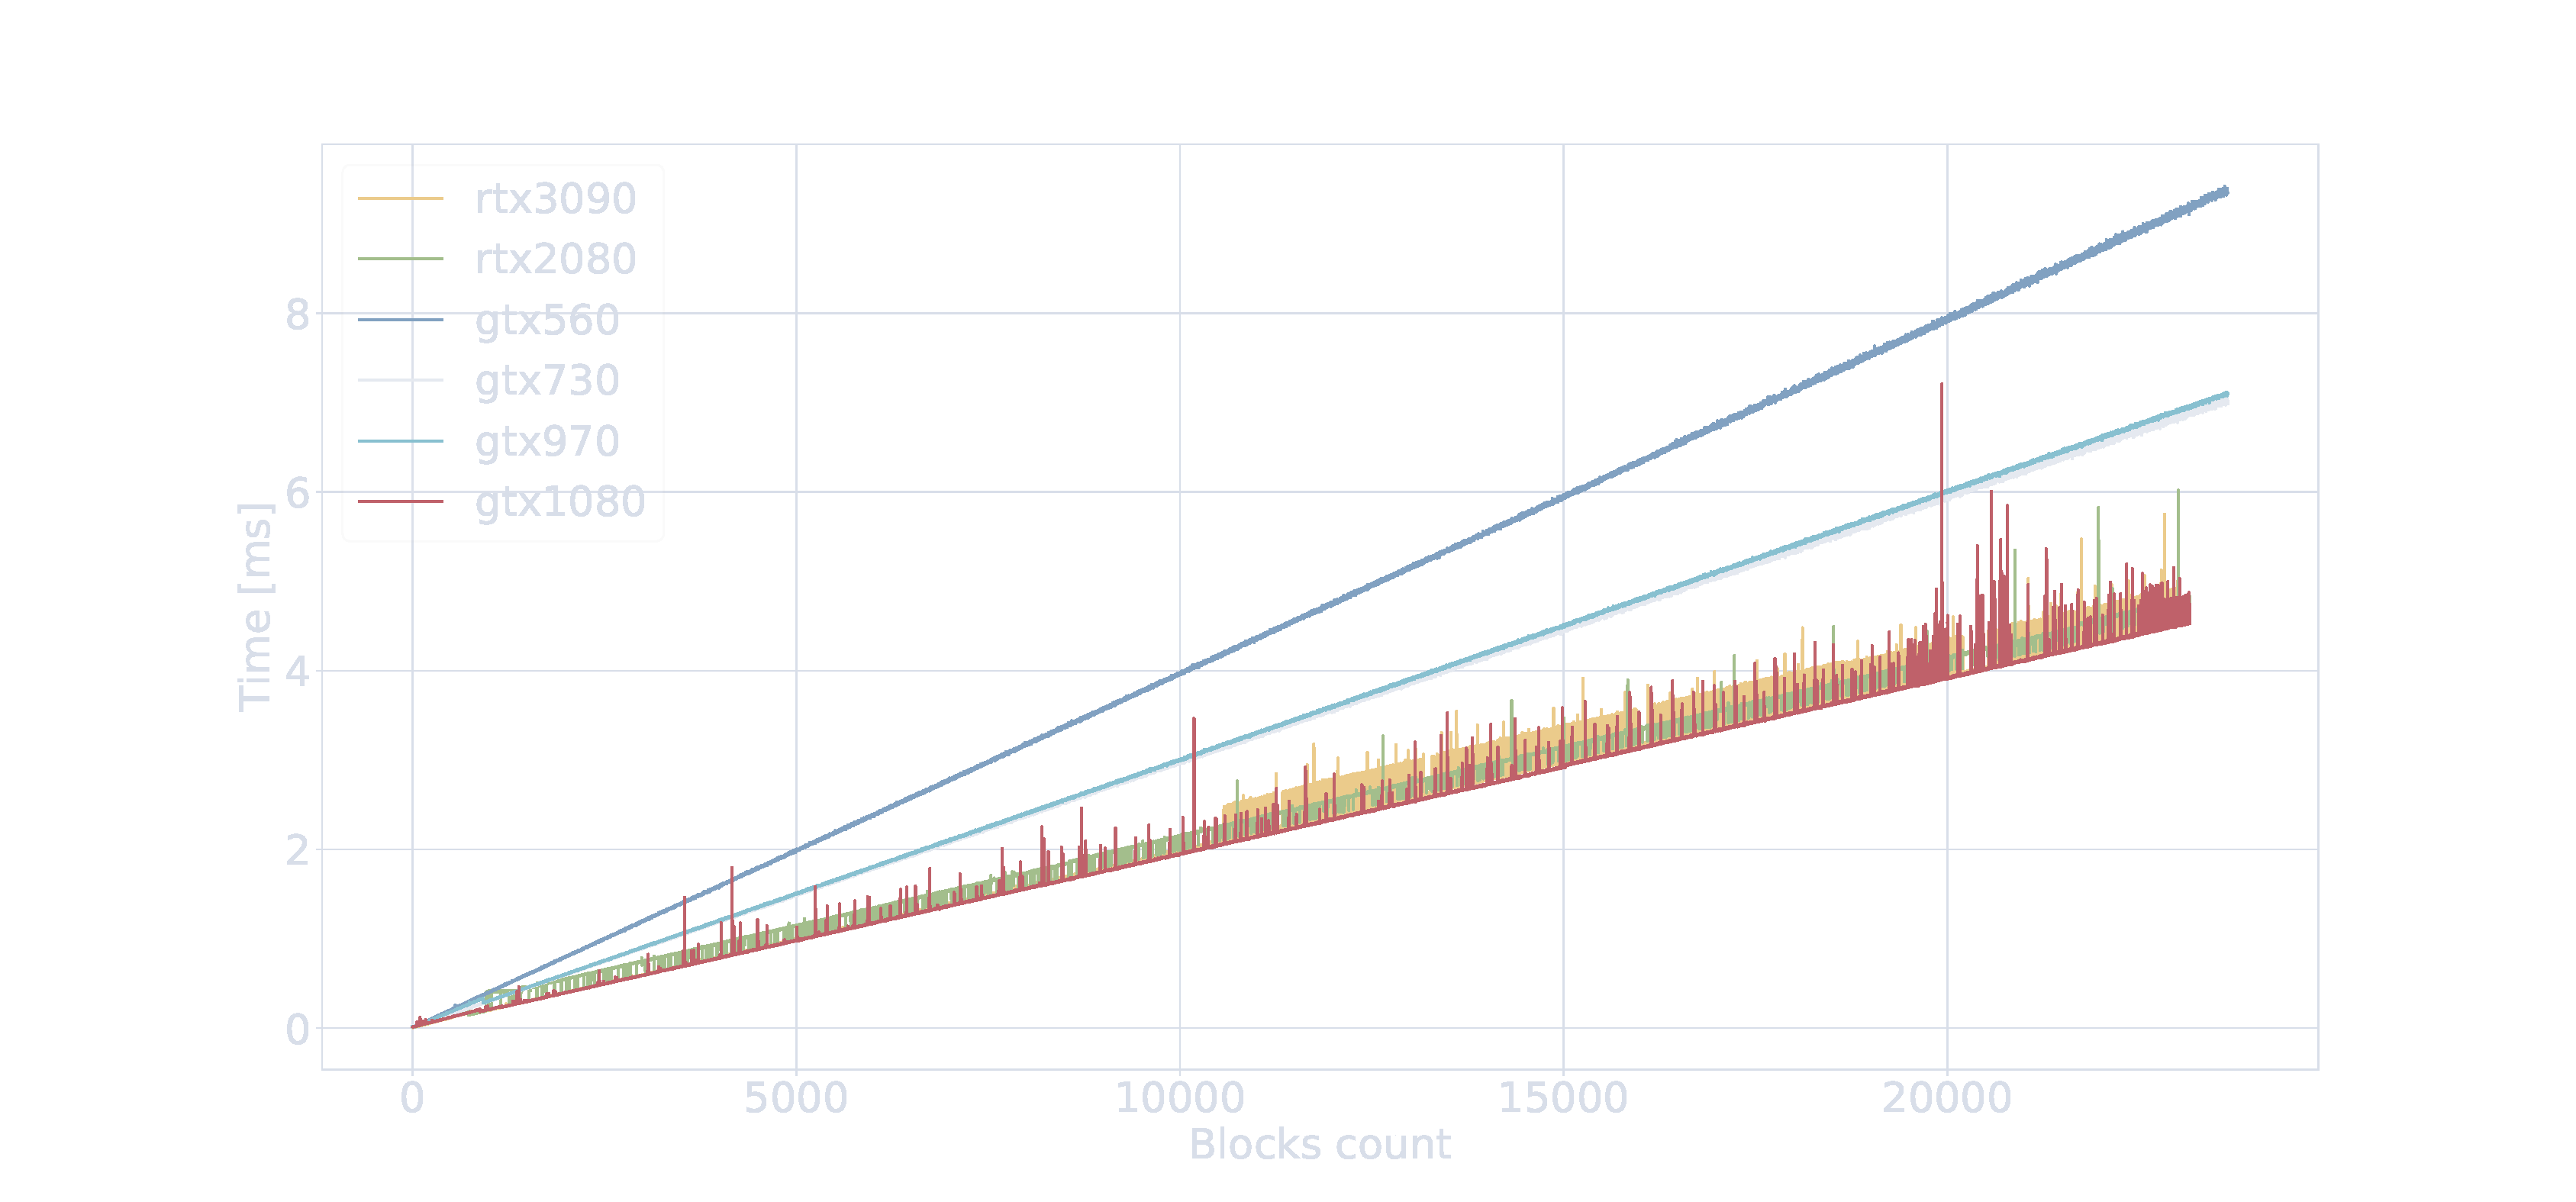
\includegraphics[width=\textwidth]{mp_elap.pdf}
	\end{figure}
\end{frame}


\begin{frame}[fragile]{Exclusive scan}{decoupled look-back}

\vspace{0.1in}

\begin{lstlisting}[showstringspaces=false]
if (blockIdx.x == 0)
  if (threadIdx.x == 0)
    store (block_statuses + blockIdx.x, 2, block_aggregate);
\end{lstlisting}
\end{frame}

\begin{frame}[fragile]{Exclusive scan}{decoupled look-back}

\vspace{0.1in}

\begin{lstlisting}[showstringspaces=false]
if (blockIdx.x != 0) 
{
  if (threadIdx.x == 0)
    store (block_statuses + blockIdx.x, 1, block_aggregate);
  
  if (threadIdx.x / WARP_SIZE == 0)
  {
    // ...
\end{lstlisting}
\end{frame}

\begin{frame}[fragile]{Exclusive scan}{decoupled look-back}

\vspace{0.1in}

\begin{lstlisting}[showstringspaces=false]
int predecessor_idx = blockIdx.x - WARP_SIZE + threadIdx.x;
data_type thread_sum = data_type ();

while (true)
{
  prev_block_status = load (block_statuses + predecessor_idx);

  while (prev_block_status.flag == 0)
    prev_block_status = load (block_statuses + predecessor_idx);
\end{lstlisting}
\end{frame}

\begin{frame}[fragile]{Exclusive scan}{decoupled look-back}

\vspace{0.1in}

\begin{lstlisting}[showstringspaces=false]
if (__all_sync (WARP_MASK, prev_block_status.flag < 2)) {
  thread_sum += prev_block_status.data;
  predecessor_idx -= WARP_SIZE;
  continue;
}
else {
  const int final_mask = 
    __ballot_sync (WARP_MASK, prev_block_status.flag > 1);

  const int rightmost_thread = WARP_SIZE - 1 - __clz (final_mask);

  thread_sum += threadIdx.x % WARP_SIZE < rightmost_thread 
              ? 0 
              : prev_block_status.data;
  break;
}
\end{lstlisting}
\end{frame}

\begin{frame}[fragile]{Exclusive scan}{decoupled look-back}

\vspace{0.1in}

\begin{lstlisting}[showstringspaces=false]
data_type aggregate = 
  WarpReduce (temp_storage.warp_reduce).Sum (thread_sum);

if (threadIdx.x == 0) {
  store (block_statuses + blockIdx.x, 2, aggregate + block_aggregate);
  prev_aggregate = aggregate;
}
\end{lstlisting}
\end{frame}

\begin{frame}[fragile]{Exclusive scan}{decoupled look-back}

\vspace{0.1in}

\begin{lstlisting}[showstringspaces=false]
      // ...
    }
  }
__syncthreads ();

const data_type reg_prev_aggregate = prev_aggregate;
for (int i = 0; i < thread_data_size; i++)
  thread_data[i] += reg_prev_aggregate;

BlockStore (temp_storage).Store (out + block_offset, thread_data);
\end{lstlisting}
\end{frame}

\begin{frame}[fragile]{Exclusive scan}{decoupled look-back}
\centering
	\begin{figure}
		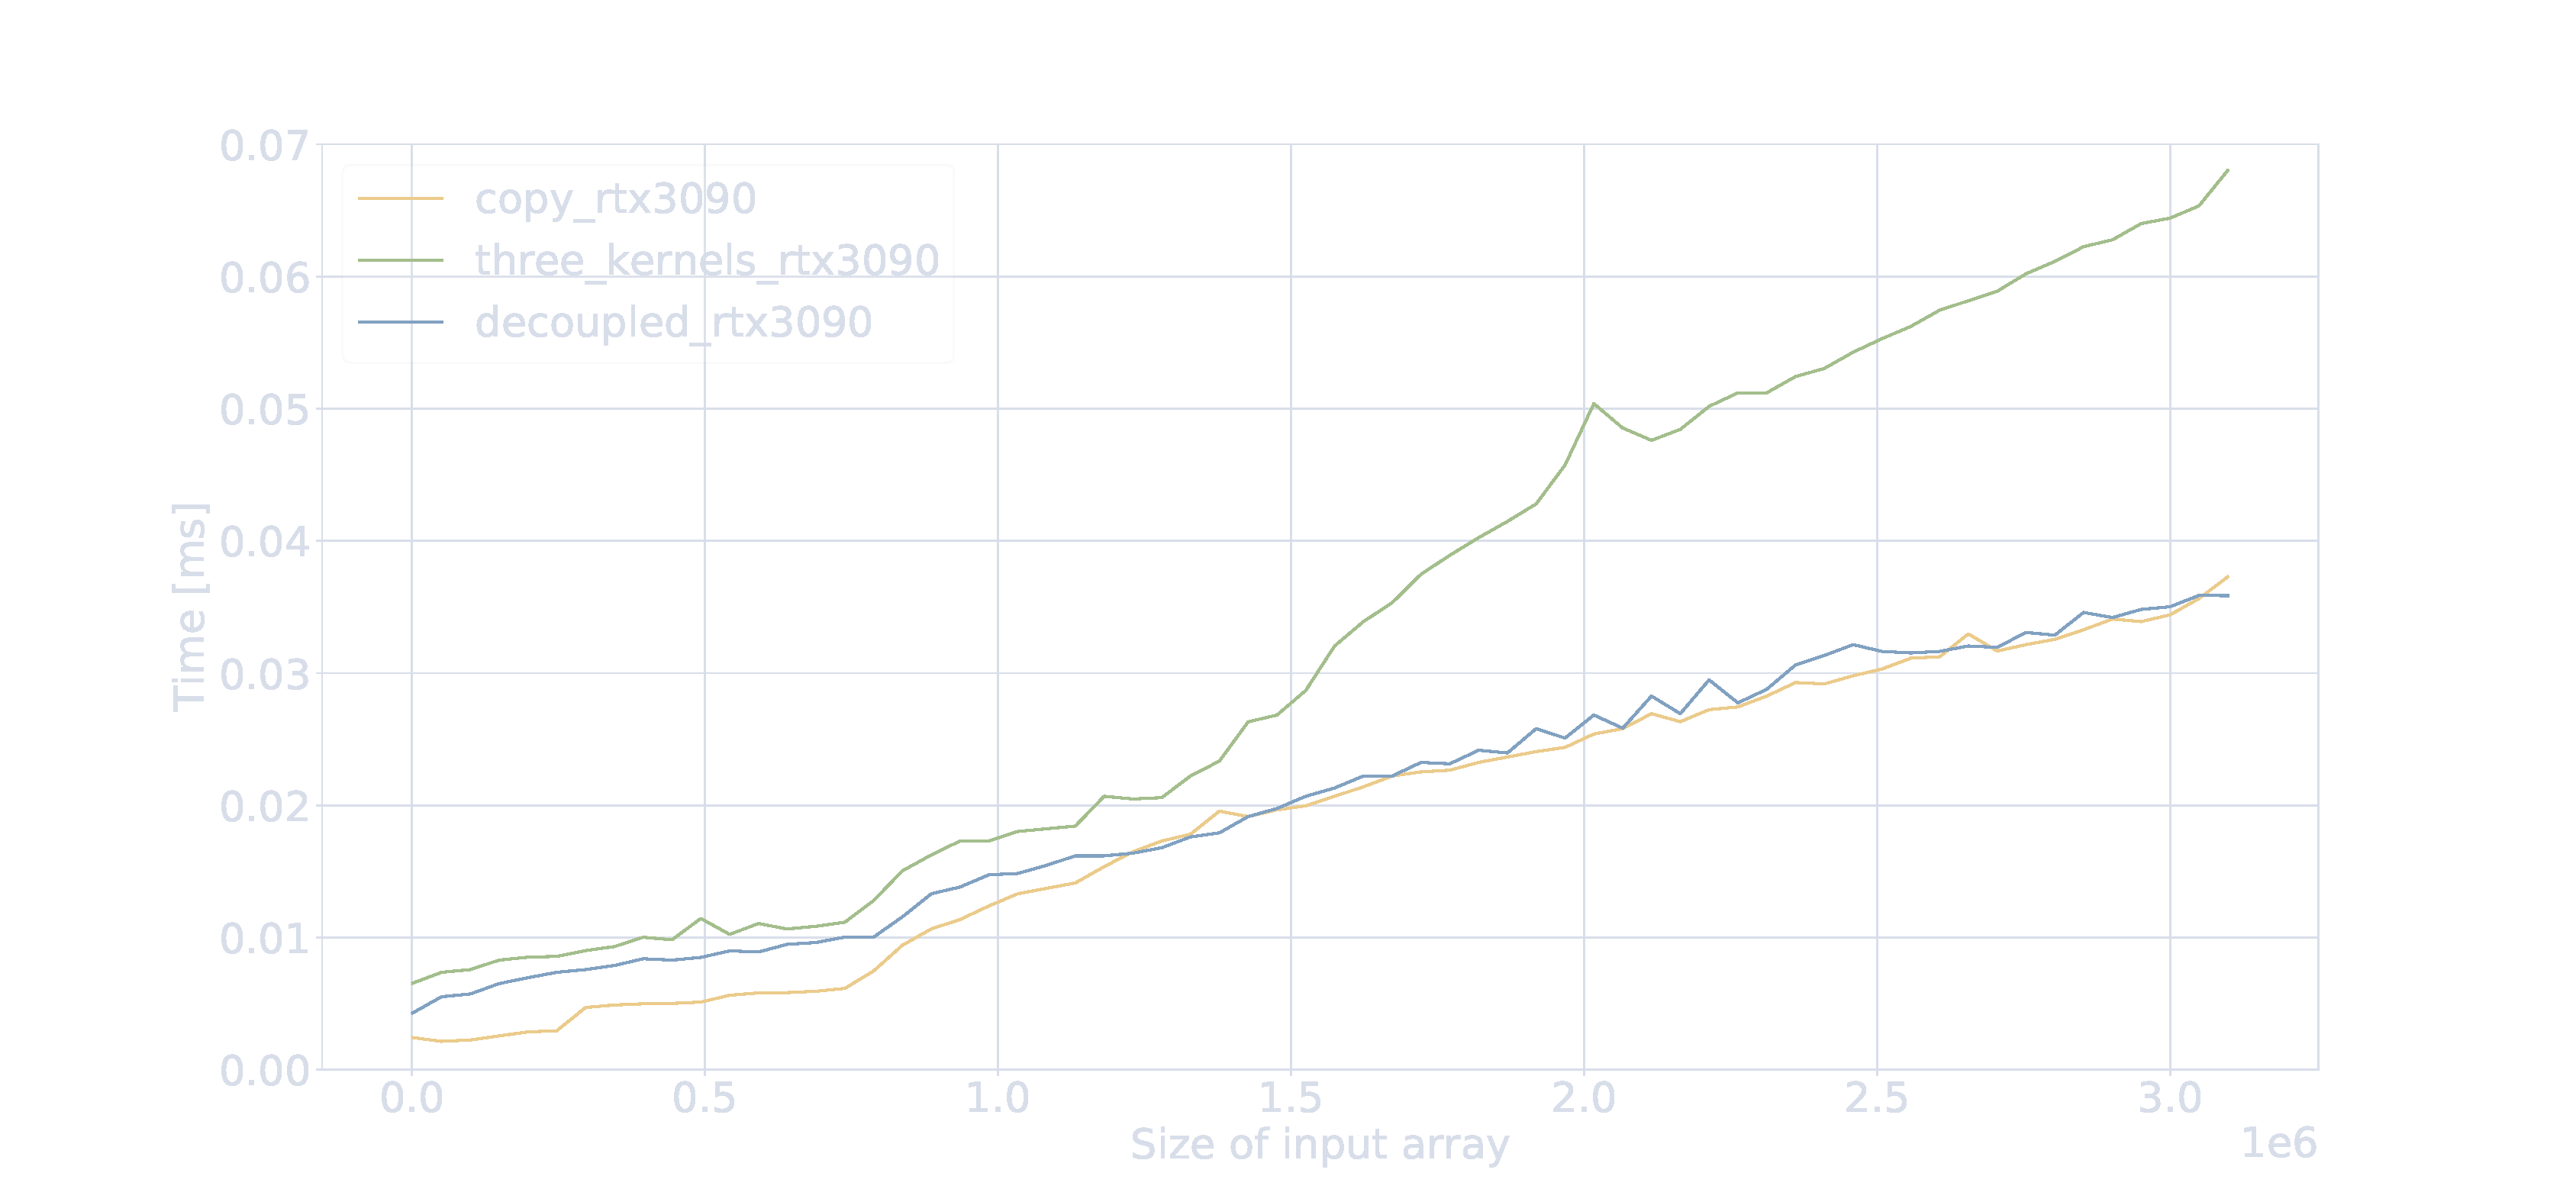
\includegraphics[width=\textwidth]{decoupled.pdf}
	\end{figure}
\end{frame}

\begin{frame}[fragile]{Exclusive scan}{single-kernel}
\centering
	\begin{figure}
		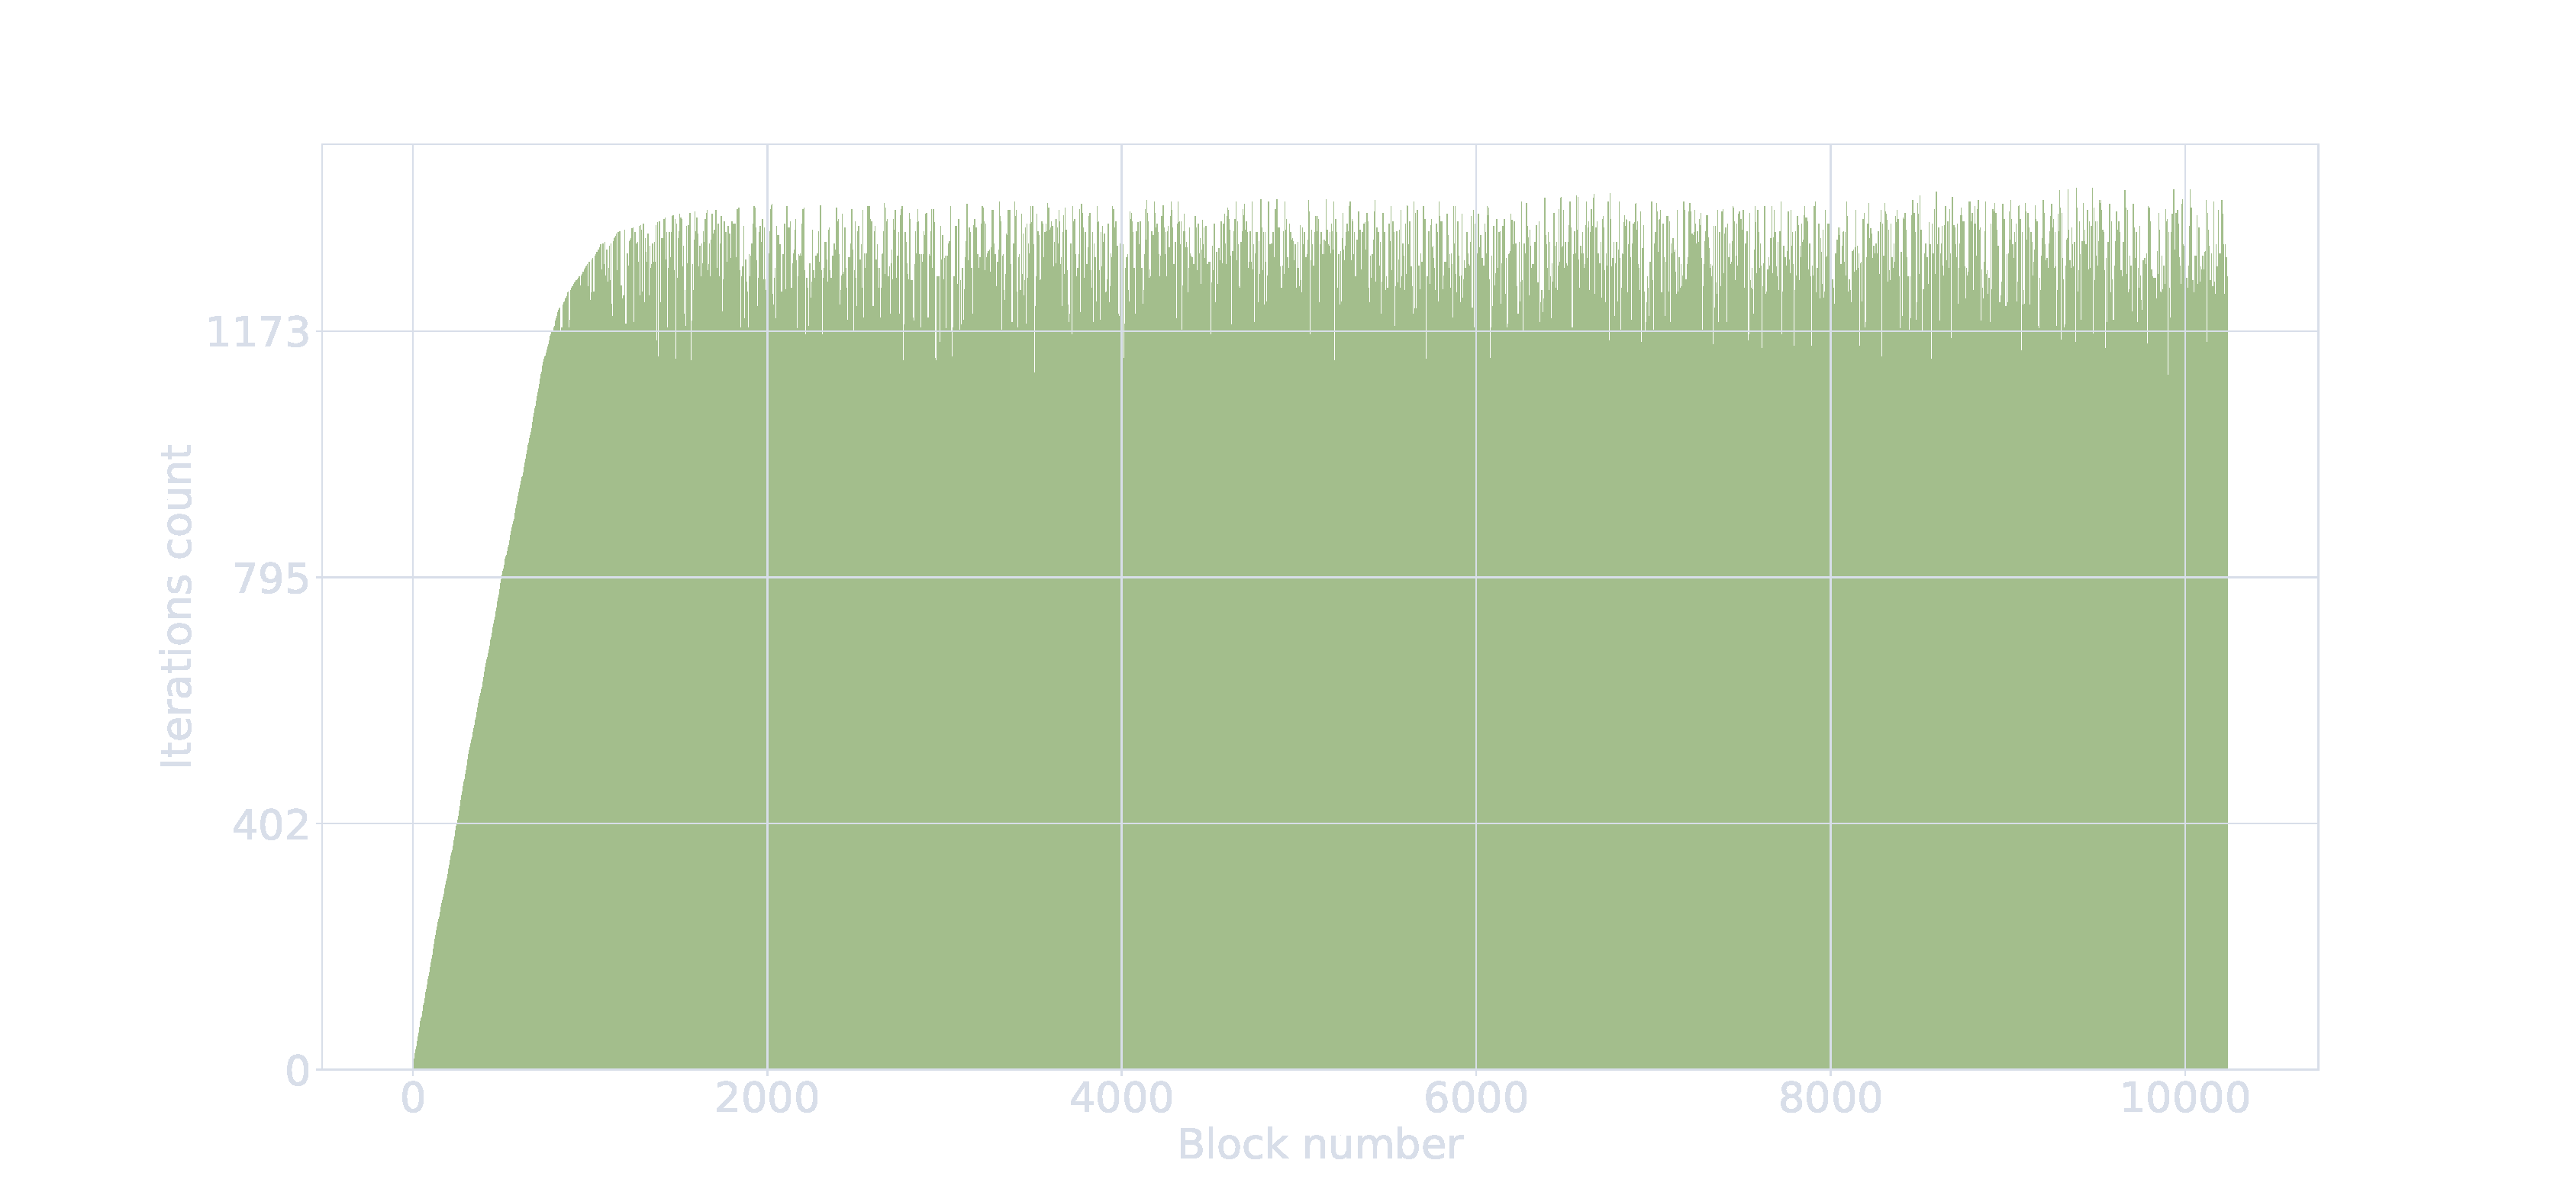
\includegraphics[width=\textwidth]{mp_hist.pdf}
	\end{figure}
\end{frame}

\begin{frame}[fragile]{Exclusive scan}{decoupled look-back}
\centering
	\begin{figure}
		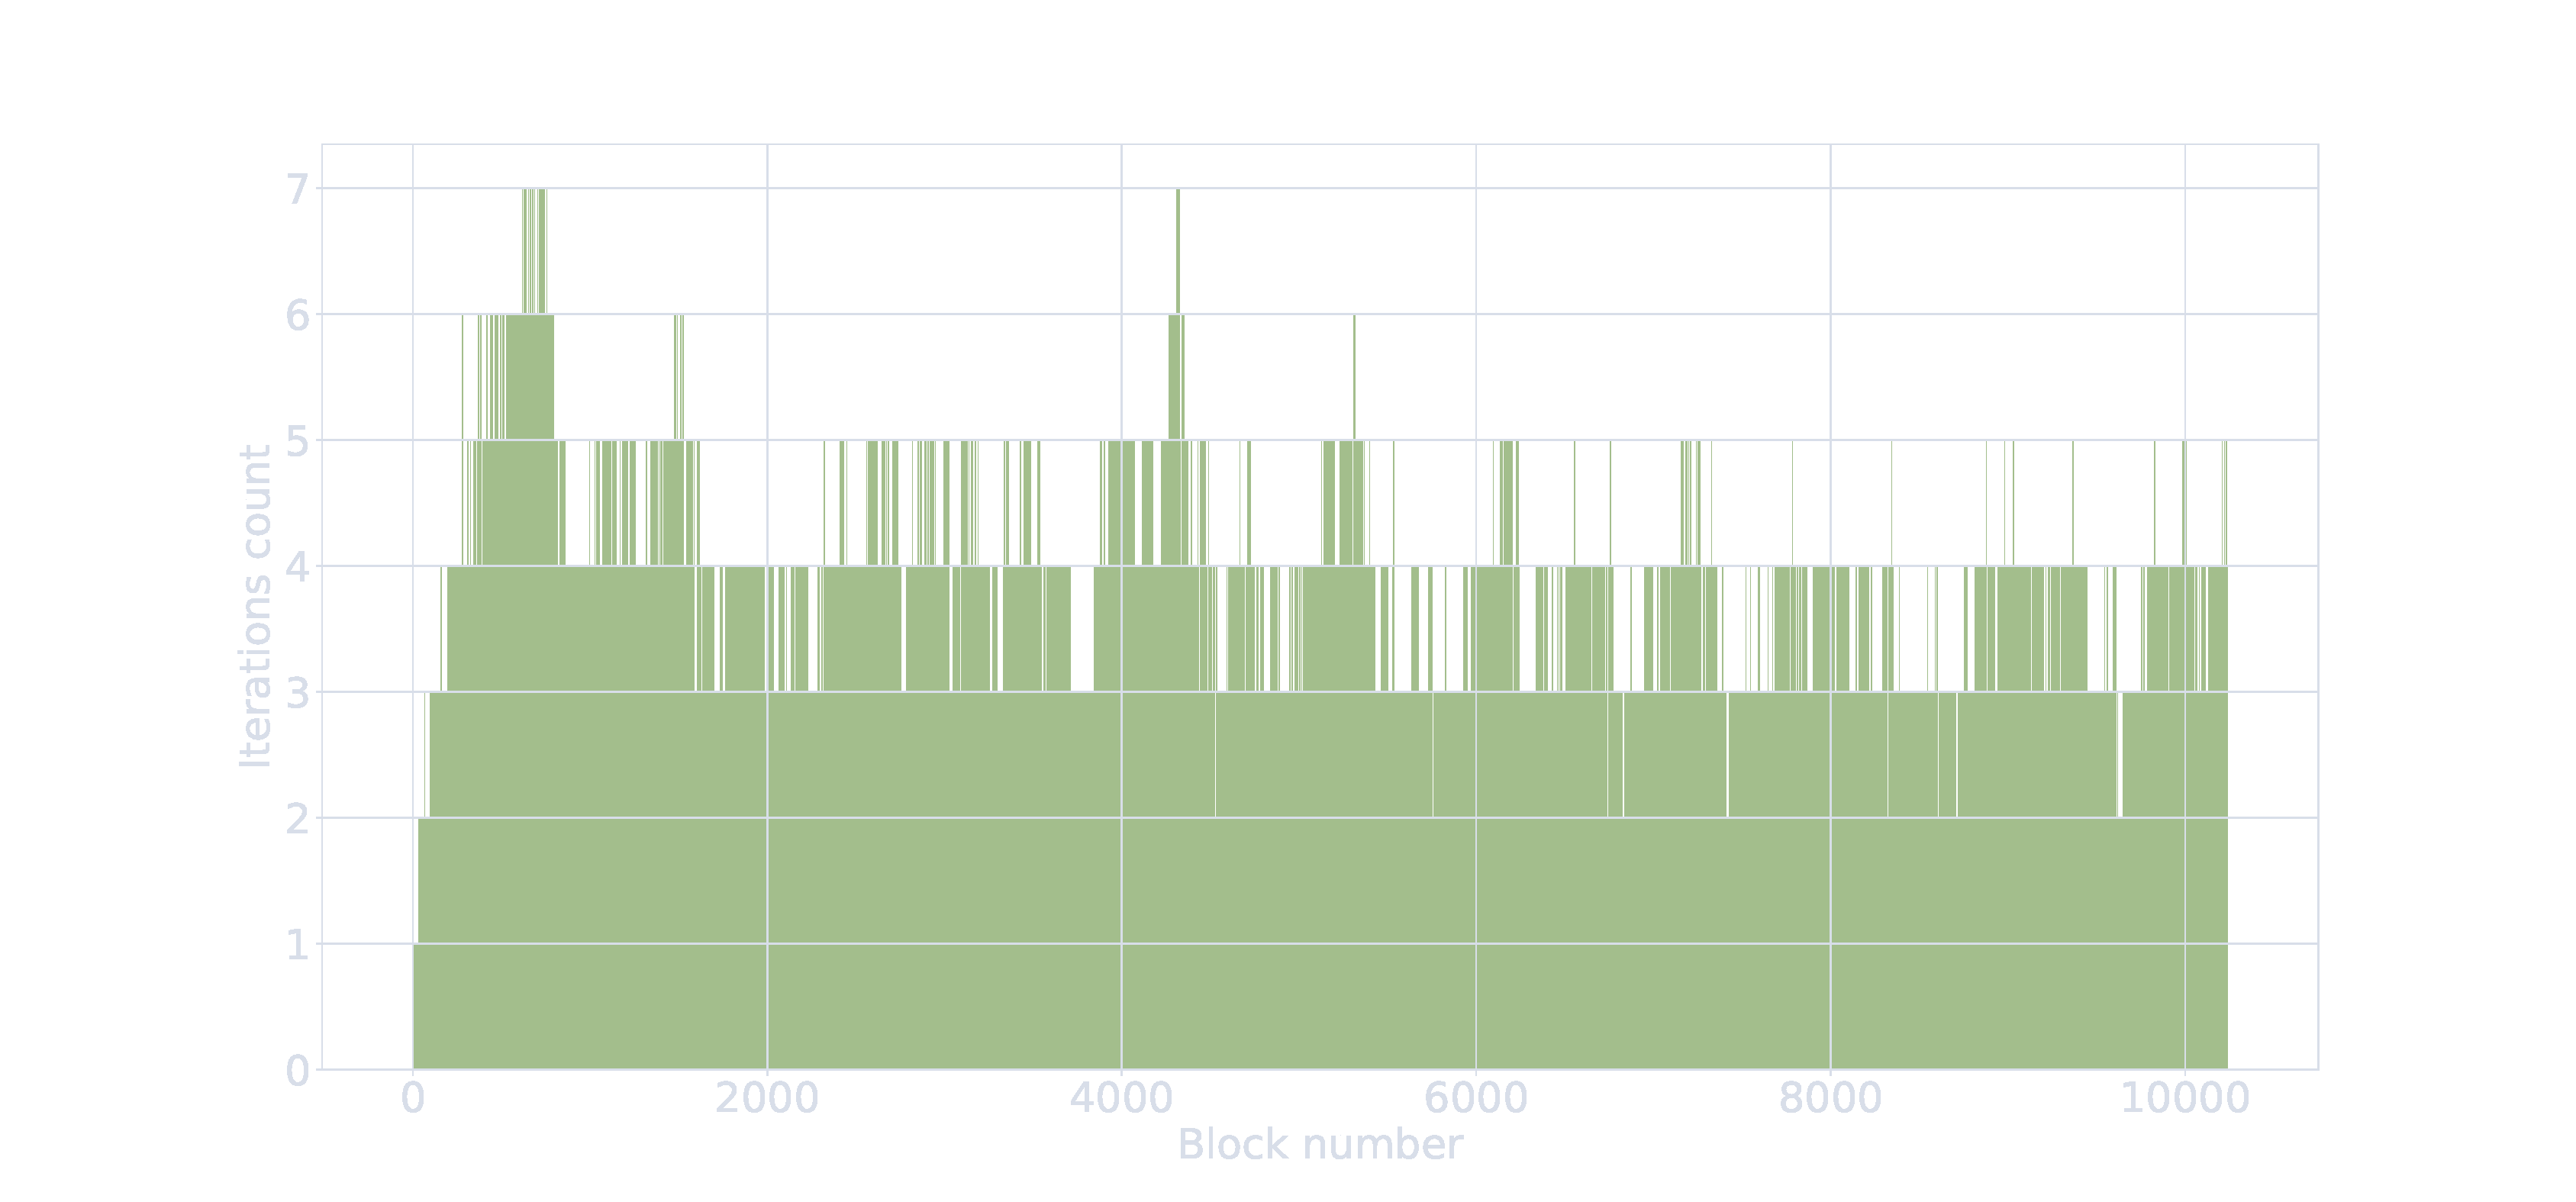
\includegraphics[width=\textwidth]{decoupled_hist.pdf}
	\end{figure}
\end{frame}

\begin{frame}[fragile]{Exclusive scan}{decoupled look-back with fence}
Fence version: \textcolor{NordYellow}{23\%} performance degradation
\centering
	\begin{figure}
		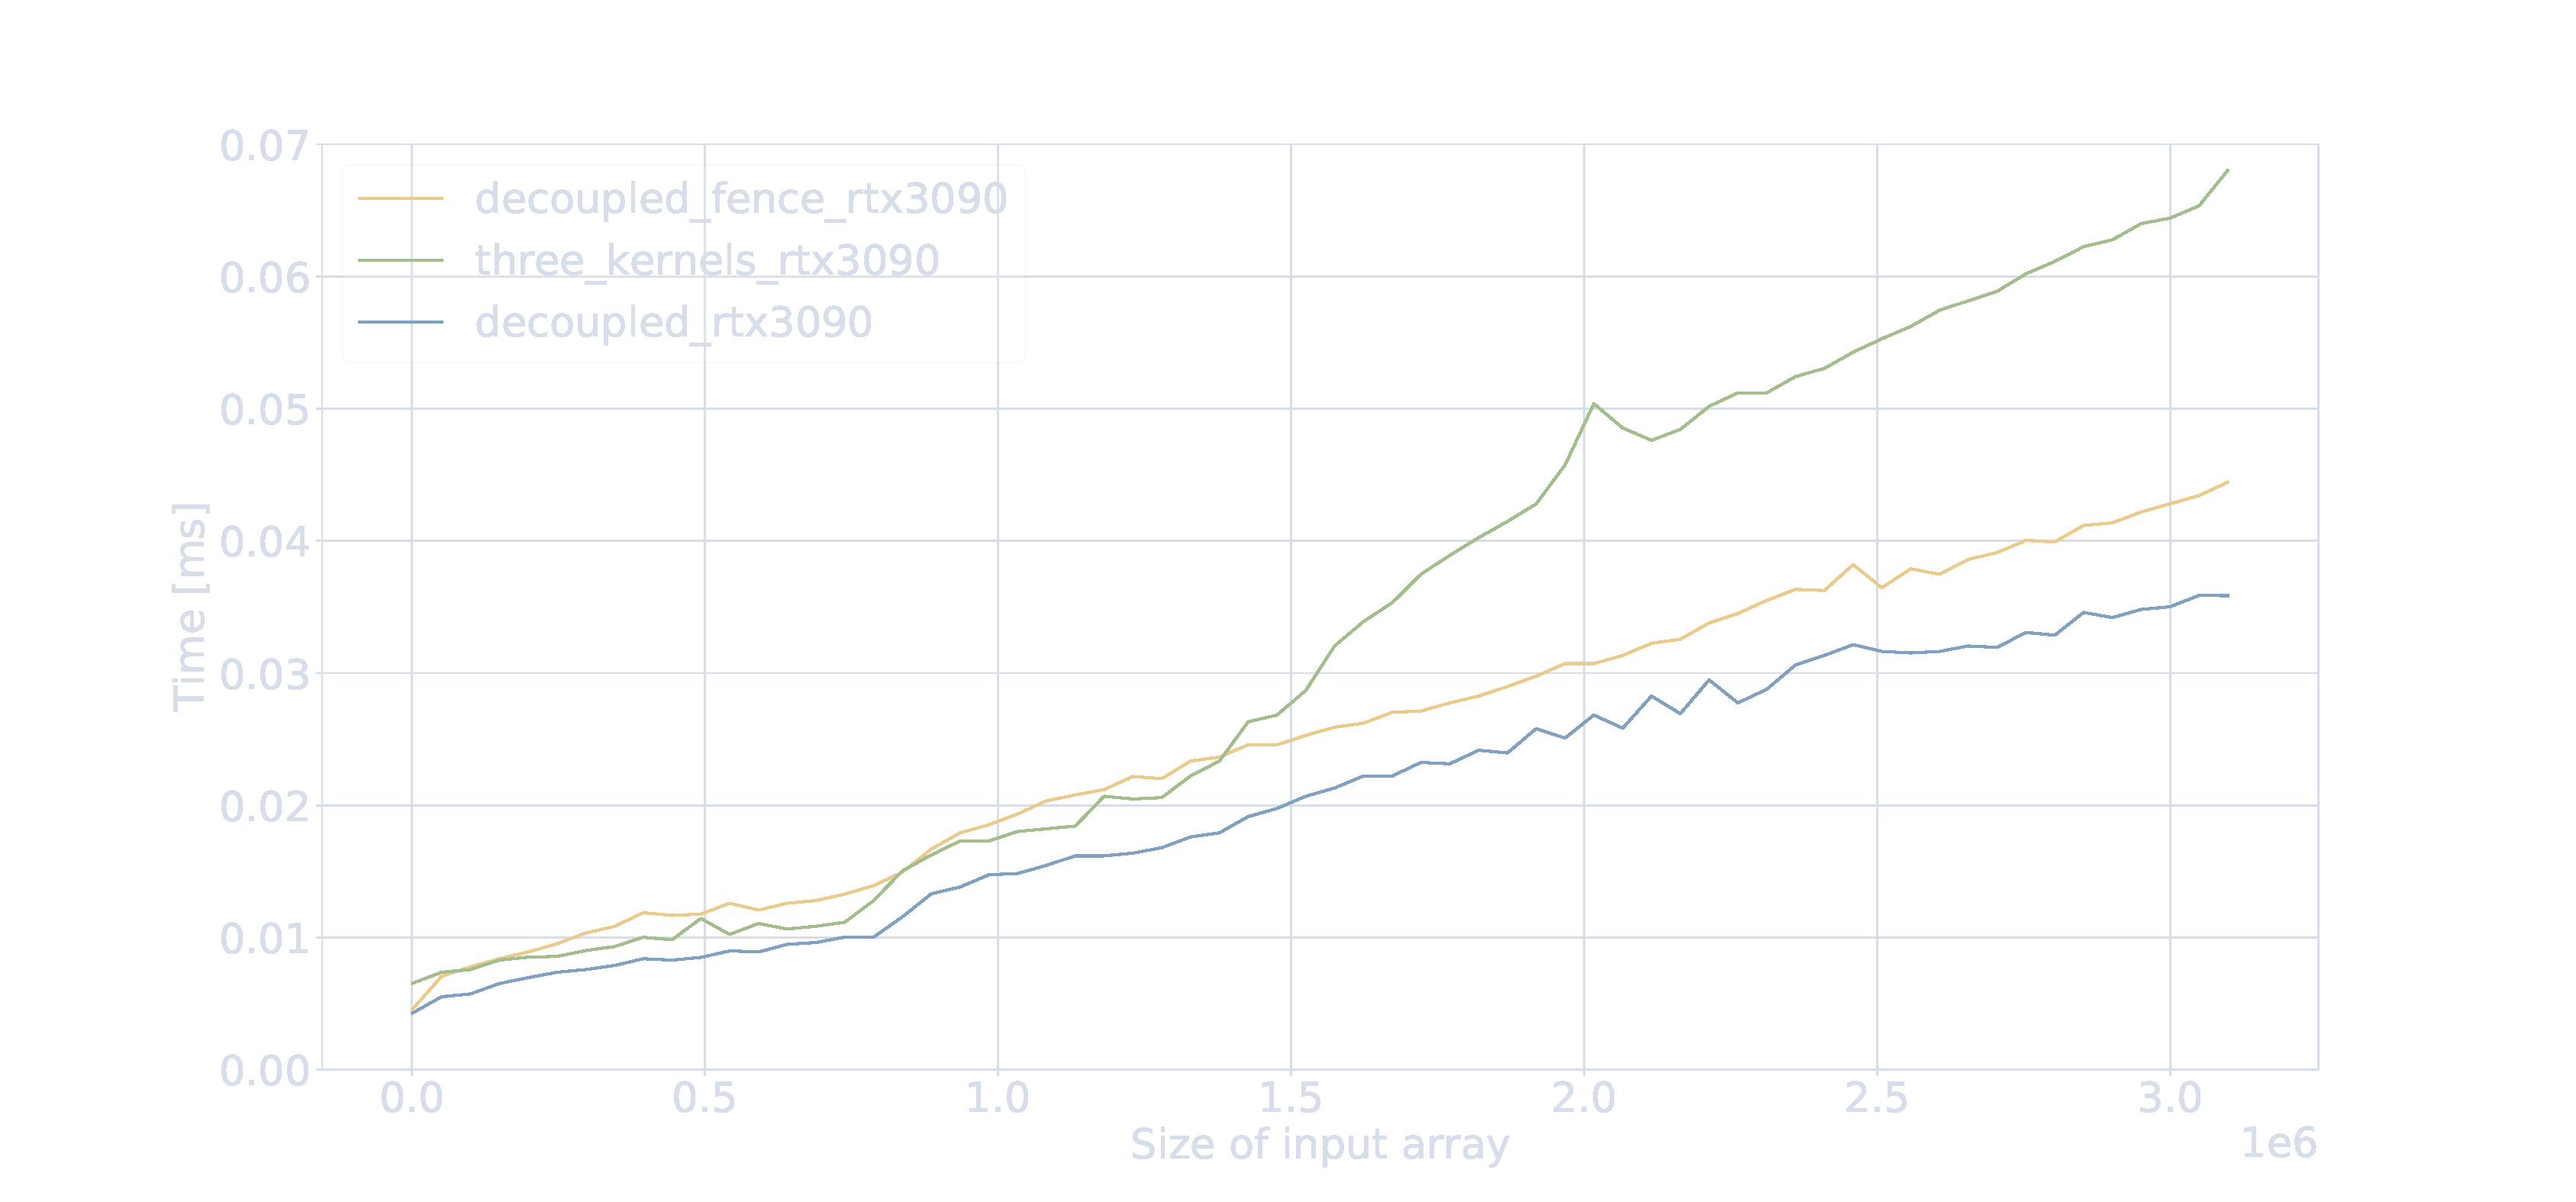
\includegraphics[width=0.9\textwidth]{decoupled_fence.pdf}
	\end{figure}
\end{frame}

\begin{frame}[fragile]{Release and Acquire Patterns}{fence}
  \begin{description}[Release pattern]
		\item[Release pattern] on a location M consists of fence followed by a 
			strong write on M in program order.

\begin{lstlisting}[]
__threadfence ();
*flag = 1; // volatile int *flag
\end{lstlisting}

		\item[Acquire pattern] on a location M consists of strong read on M followed
			by a fence in program order.

\begin{lstlisting}[]
int reg = *flag; // volatile int *flag
__threadfence ();
\end{lstlisting}
	\end{description}

\end{frame}

\begin{frame}{Definitions}
  \begin{description}[Memory operation]
  \item[Read operation]
    All variants of \textcolor{NordYellow}{ld} instruction and \textcolor{NordYellow}{atom} instruction.
  \item[Write operation]
    All variants of \textcolor{NordYellow}{st} instruction and \textcolor{NordYellow}{atom} instruction.
  \item[Memory operation]
    A \textcolor{NordYellow}{read} or \textcolor{NordYellow}{write} operation.
  \end{description}
\end{frame}

\begin{frame}{Definitions}
  \begin{description}[Memory operation]
  \item[Read operation]
    All variants of \textcolor{NordYellow}{ld} instruction and \textcolor{NordYellow}{atom} instruction.
  \item[Write operation]
    All variants of \textcolor{NordYellow}{st} instruction and \textcolor{NordYellow}{atom} instruction.
  \item[Memory operation]
    A \textcolor{NordYellow}{read} or \textcolor{NordYellow}{write} operation.
  \item[Strong operation]
		A \textcolor{NordYellow}{fence} operation, or a memory operation with a \\
			\textcolor{NordYellow}{.relaxed}, \textcolor{NordYellow}{.acquire}, 
			\textcolor{NordYellow}{.release}, \textcolor{NordYellow}{.acq\_rel} or 
			\textcolor{NordYellow}{.volatile} qualifier.
  \end{description}
\end{frame}

\begin{frame}[fragile]{Release and Acquire Patterns}{acquire/release operations}
  \begin{description}[Release pattern]
		\item[Release pattern] on a location M consists of a release operation on M.

\begin{lstlisting}[]
__device__ void store_release (int * flag, int val) 
{
  asm volatile (
    "st.release.gpu.b32 [%0], %1;" 
 :: "l"(flag),"r"(val) : "memory"); 
}
\end{lstlisting}

		\item[Acquire pattern] on a location M consists of an acquire operation on M.

\begin{lstlisting}[]
__device__ int load_acquire (int * flag) 
{
  int reg;
  asm volatile (
    "ld.acquire.gpu.b32 %0, [%1];" 
  : "=r"(reg) : "l"(flag) : "memory"); 
  return reg;
}
\end{lstlisting}
	\end{description}

\end{frame}

\begin{frame}[fragile]{Release and Acquire Patterns}{acquire/release operations}
	\begin{columns}
			\begin{column}{0.4\textwidth}
\begin{lstlisting}[language={SASS},title={st.release.gpu}]
MEMBAR.ALL.GPU
ST.E.STRONG.GPU [UR4], R0
\end{lstlisting}
			\end{column}
			\begin{column}{0.4\textwidth}
\begin{lstlisting}[language={SASS},title={ld.acquire.gpu}]
LD.E.STRONG.GPU R0, [UR4]
CCTL.IVALL
\end{lstlisting}
			\end{column}
	\end{columns}
\end{frame}

\begin{frame}[fragile]{Release and Acquire Patterns}{libcu++}
\begin{lstlisting}[]
__device__ void old_writer (
    int n, volatile int * flag, int * data, int *result) { 
  for (int i = 0; i < n; i++)
    data[i] = i + 1;

  __threadfence ();
  *flag = 1;
}
\end{lstlisting}
\begin{lstlisting}[]
__device__ void new_writer (
    int n, atomic<int> &flag, int * data, int *result) { 
  for (int i = 0; i < n; i++)
    data[i] = i + 1;

  flag.store (1, memory_order_release);
}
\end{lstlisting}
\end{frame}


\begin{frame}[fragile]{Reduce}{sequential version}
\vspace{0.1in}
Reduce produces a single aggregate from a list of input elements.
\vspace{0.3in}
\begin{columns}[T]
	\begin{column}{0.35\textwidth}

\begin{lstlisting}[showstringspaces=false]
int sum = 0;
for (int i = 0; i < n; i++)
  sum += in[i];
*out = sum;
\end{lstlisting}
	\end{column}
	\begin{column}{0.4\textwidth}
		\begin{tikzpicture}[square/.style={regular polygon,regular polygon sides=4}]
			\node[text=NordWhite] (in0) {in};
		  \foreach[count=\i] \invalue in {1,0,1,1,0,1} {
			  \pgfmathsetmacro\prev{int(\i - 1)}
				\node[fill=NordBlue, text=NordDarkBlack, right of=in\prev,square] (in\i) {\invalue};
			}
			\node[text=NordWhite,below of=in0] (out0) {out};
			\node[fill=NordGreen, text=NordDarkBlack, right of=out0,square] (out1) {4};
		\end{tikzpicture}
	\end{column}
\end{columns}
\end{frame}


\begin{frame}[fragile]{Device reduction}{}
\begin{lstlisting}[showstringspaces=false]
reduce<<<blocks, block_size>>> (in, block_results);
reduce_block_results<<<1, block_size>>> (
  blocks, block_results, block_results);
\end{lstlisting}
\end{frame}


\begin{frame}[fragile]{Device reduction}{}
\begin{lstlisting}[showstringspaces=false]
// .. block-wide reduce ..

if (threadIdx.x == 0)
  {
    block_results[blockIdx.x] = block_result;
    __threadfence ();

    const int prev_count = atomicAdd (count, 1);
    temp_storage.need_to_perform_final_reduce 
      = prev_count == gridDim.x - 1;
}

\end{lstlisting}
\end{frame}

\begin{frame}[fragile]{Device reduction}{performance}
Single-kernel version: $\approx$ \textcolor{NordYellow}{4\%} performance improvement
\centering
	\begin{figure}
		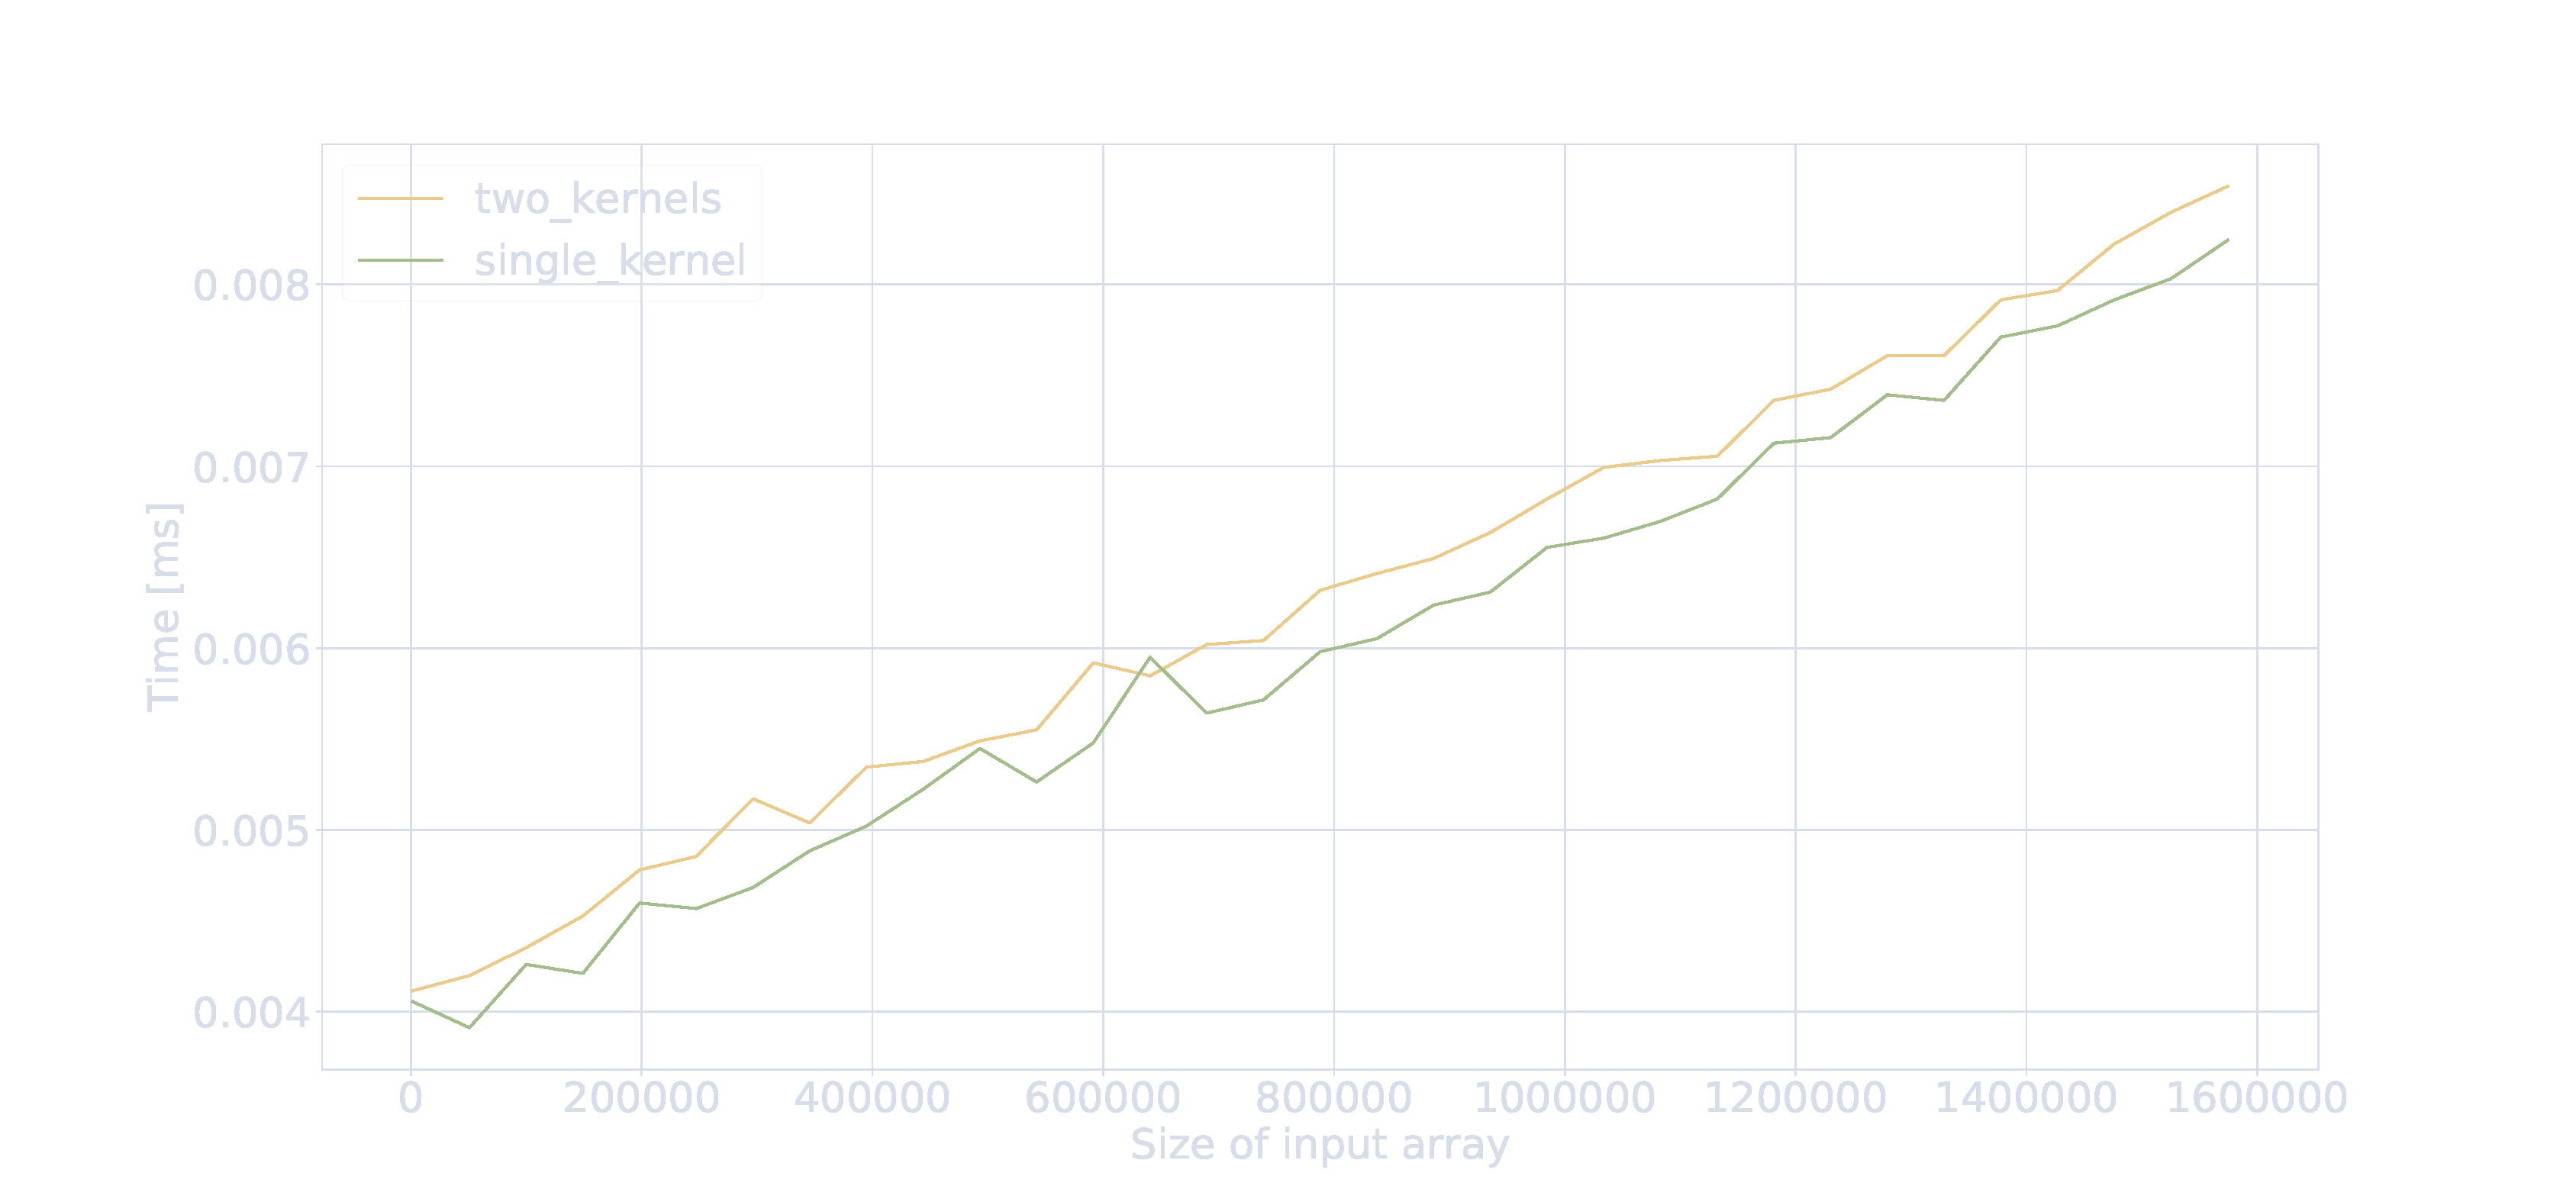
\includegraphics[width=0.9\textwidth]{reduce.pdf}
	\end{figure}
\end{frame}

\begin{frame}[fragile]{Device reduction}{}
\begin{lstlisting}[showstringspaces=false]
// .. block-wide reduce ..

if (threadIdx.x == 0)
  {
    block_results[blockIdx.x] = block_result;

    const int prev_count = 
      count->fetch_add (1, cuda::std::memory_order_release);

    temp_storage.need_to_perform_final_reduce 
      = prev_count == gridDim.x - 1;
}

\end{lstlisting}
\end{frame}

\begin{frame}[fragile]{Device reduction}{performance}
\centering
	\begin{figure}
		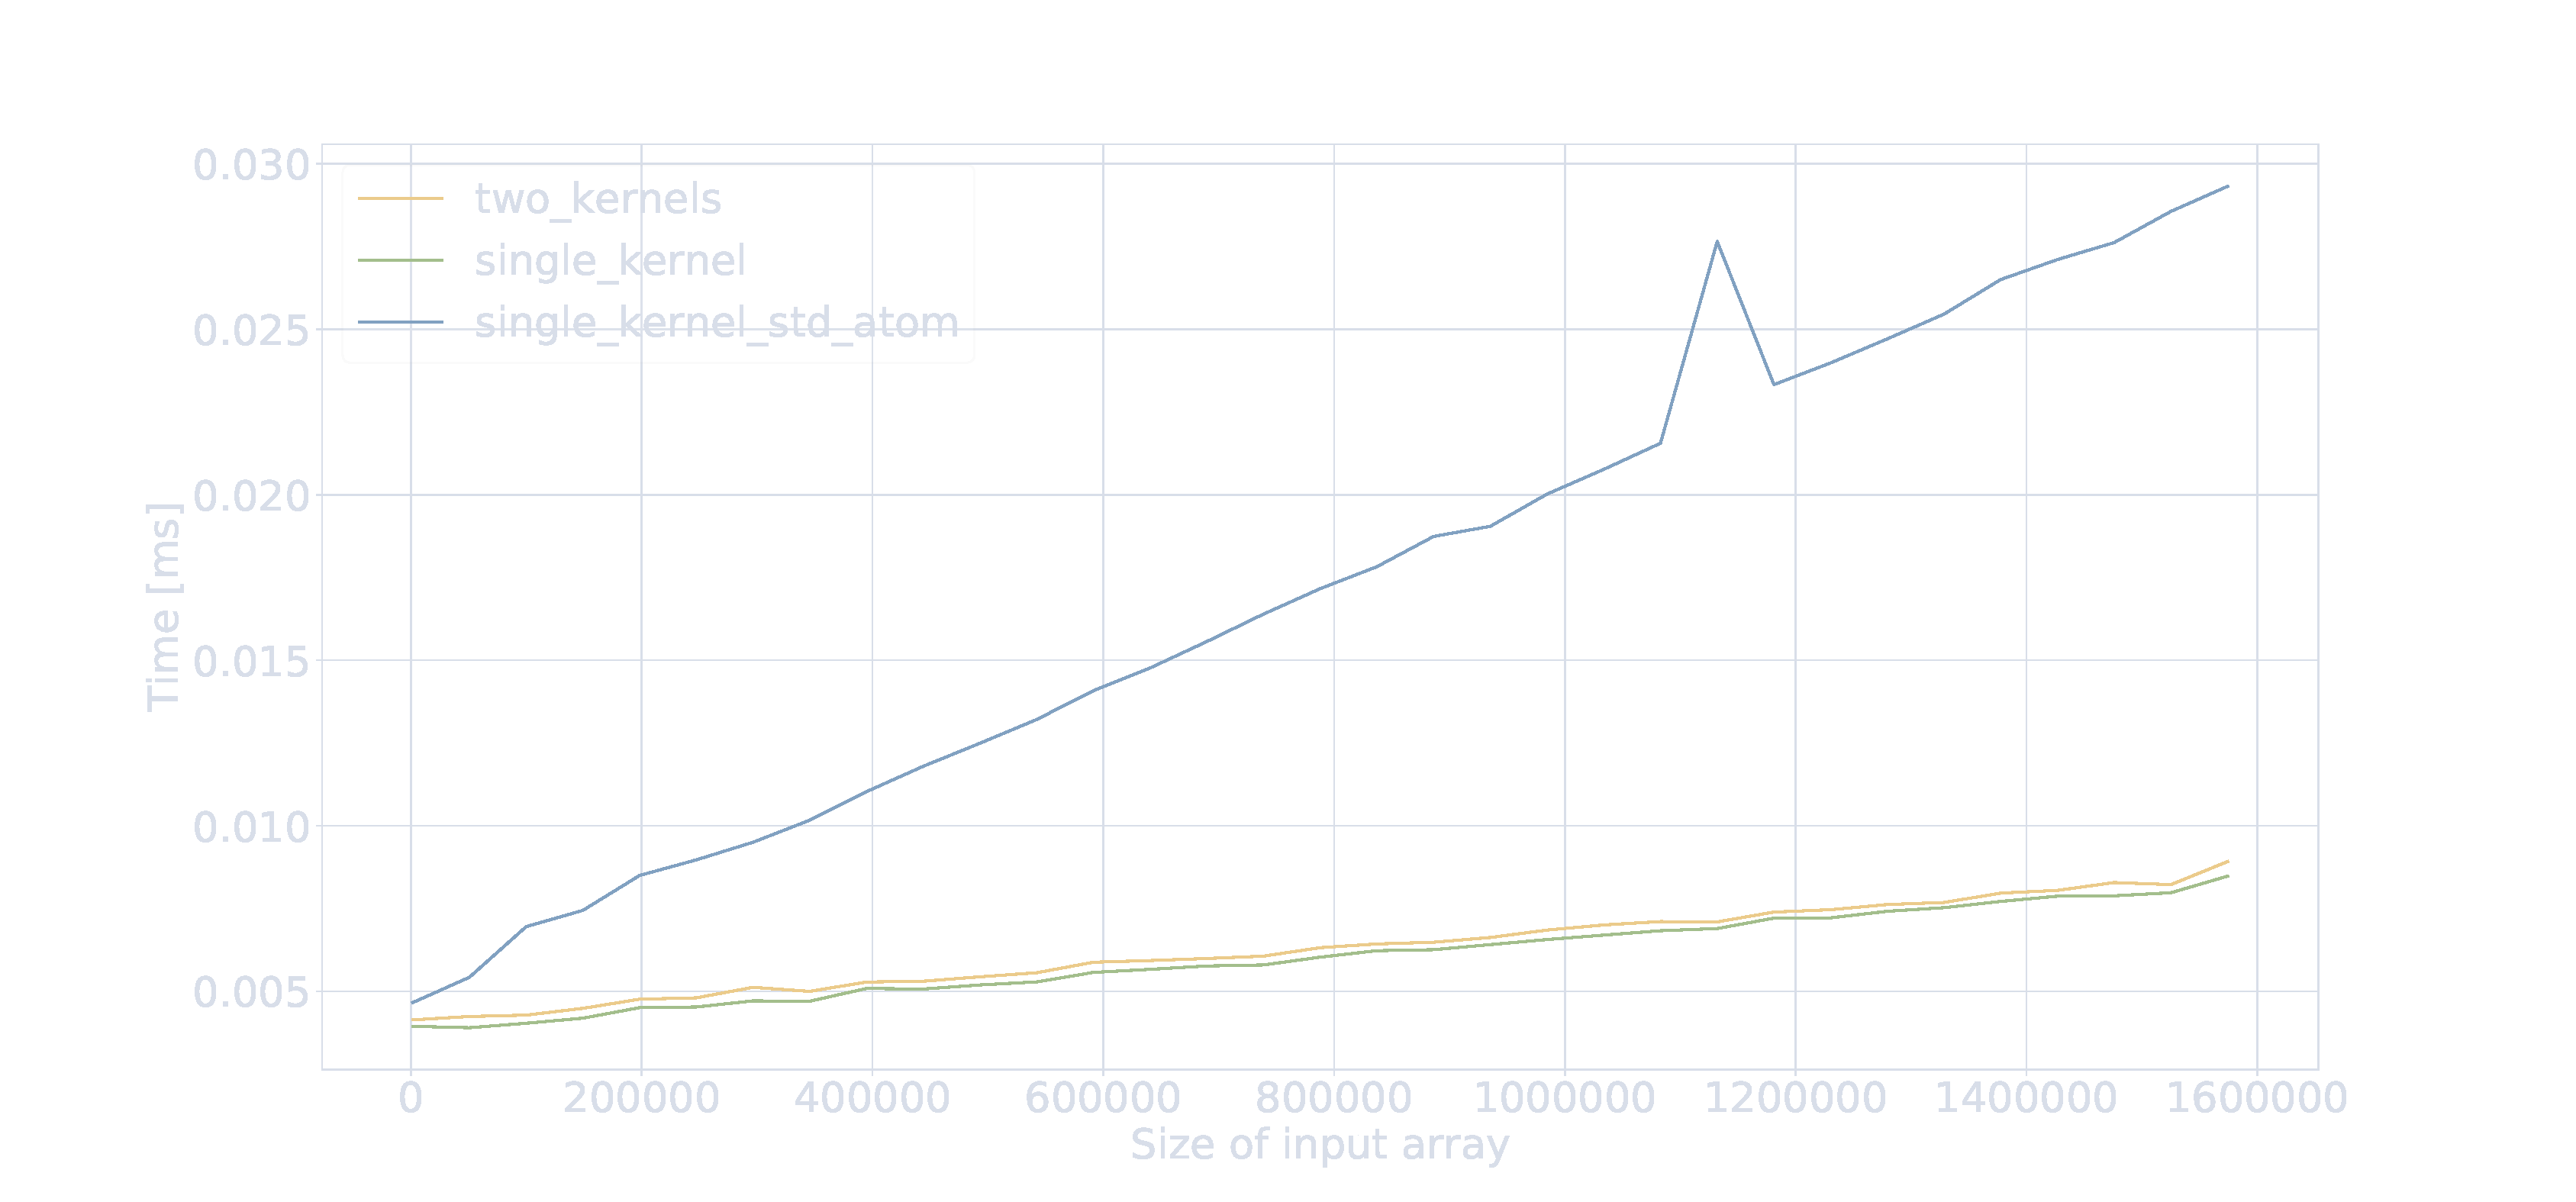
\includegraphics[width=0.9\textwidth]{reduce_std_atom.pdf}
	\end{figure}
\end{frame}

\begin{frame}[fragile]{Device reduction}{}
\begin{lstlisting}[showstringspaces=false]
// CUDA C++, __host__ __device__.
// Strictly conforming to the C++ Standard.
#include <cuda/std/atomic>
cuda::std::atomic<int> x;

// CUDA C++, __host__ __device__.
// Conforming extensions to the C++ Standard.
#include <cuda/atomic>
cuda::atomic<int, cuda::thread_scope_block> x;
\end{lstlisting}
\end{frame}

\begin{frame}[fragile]{Device reduction}{performance}
\centering
	\begin{figure}
		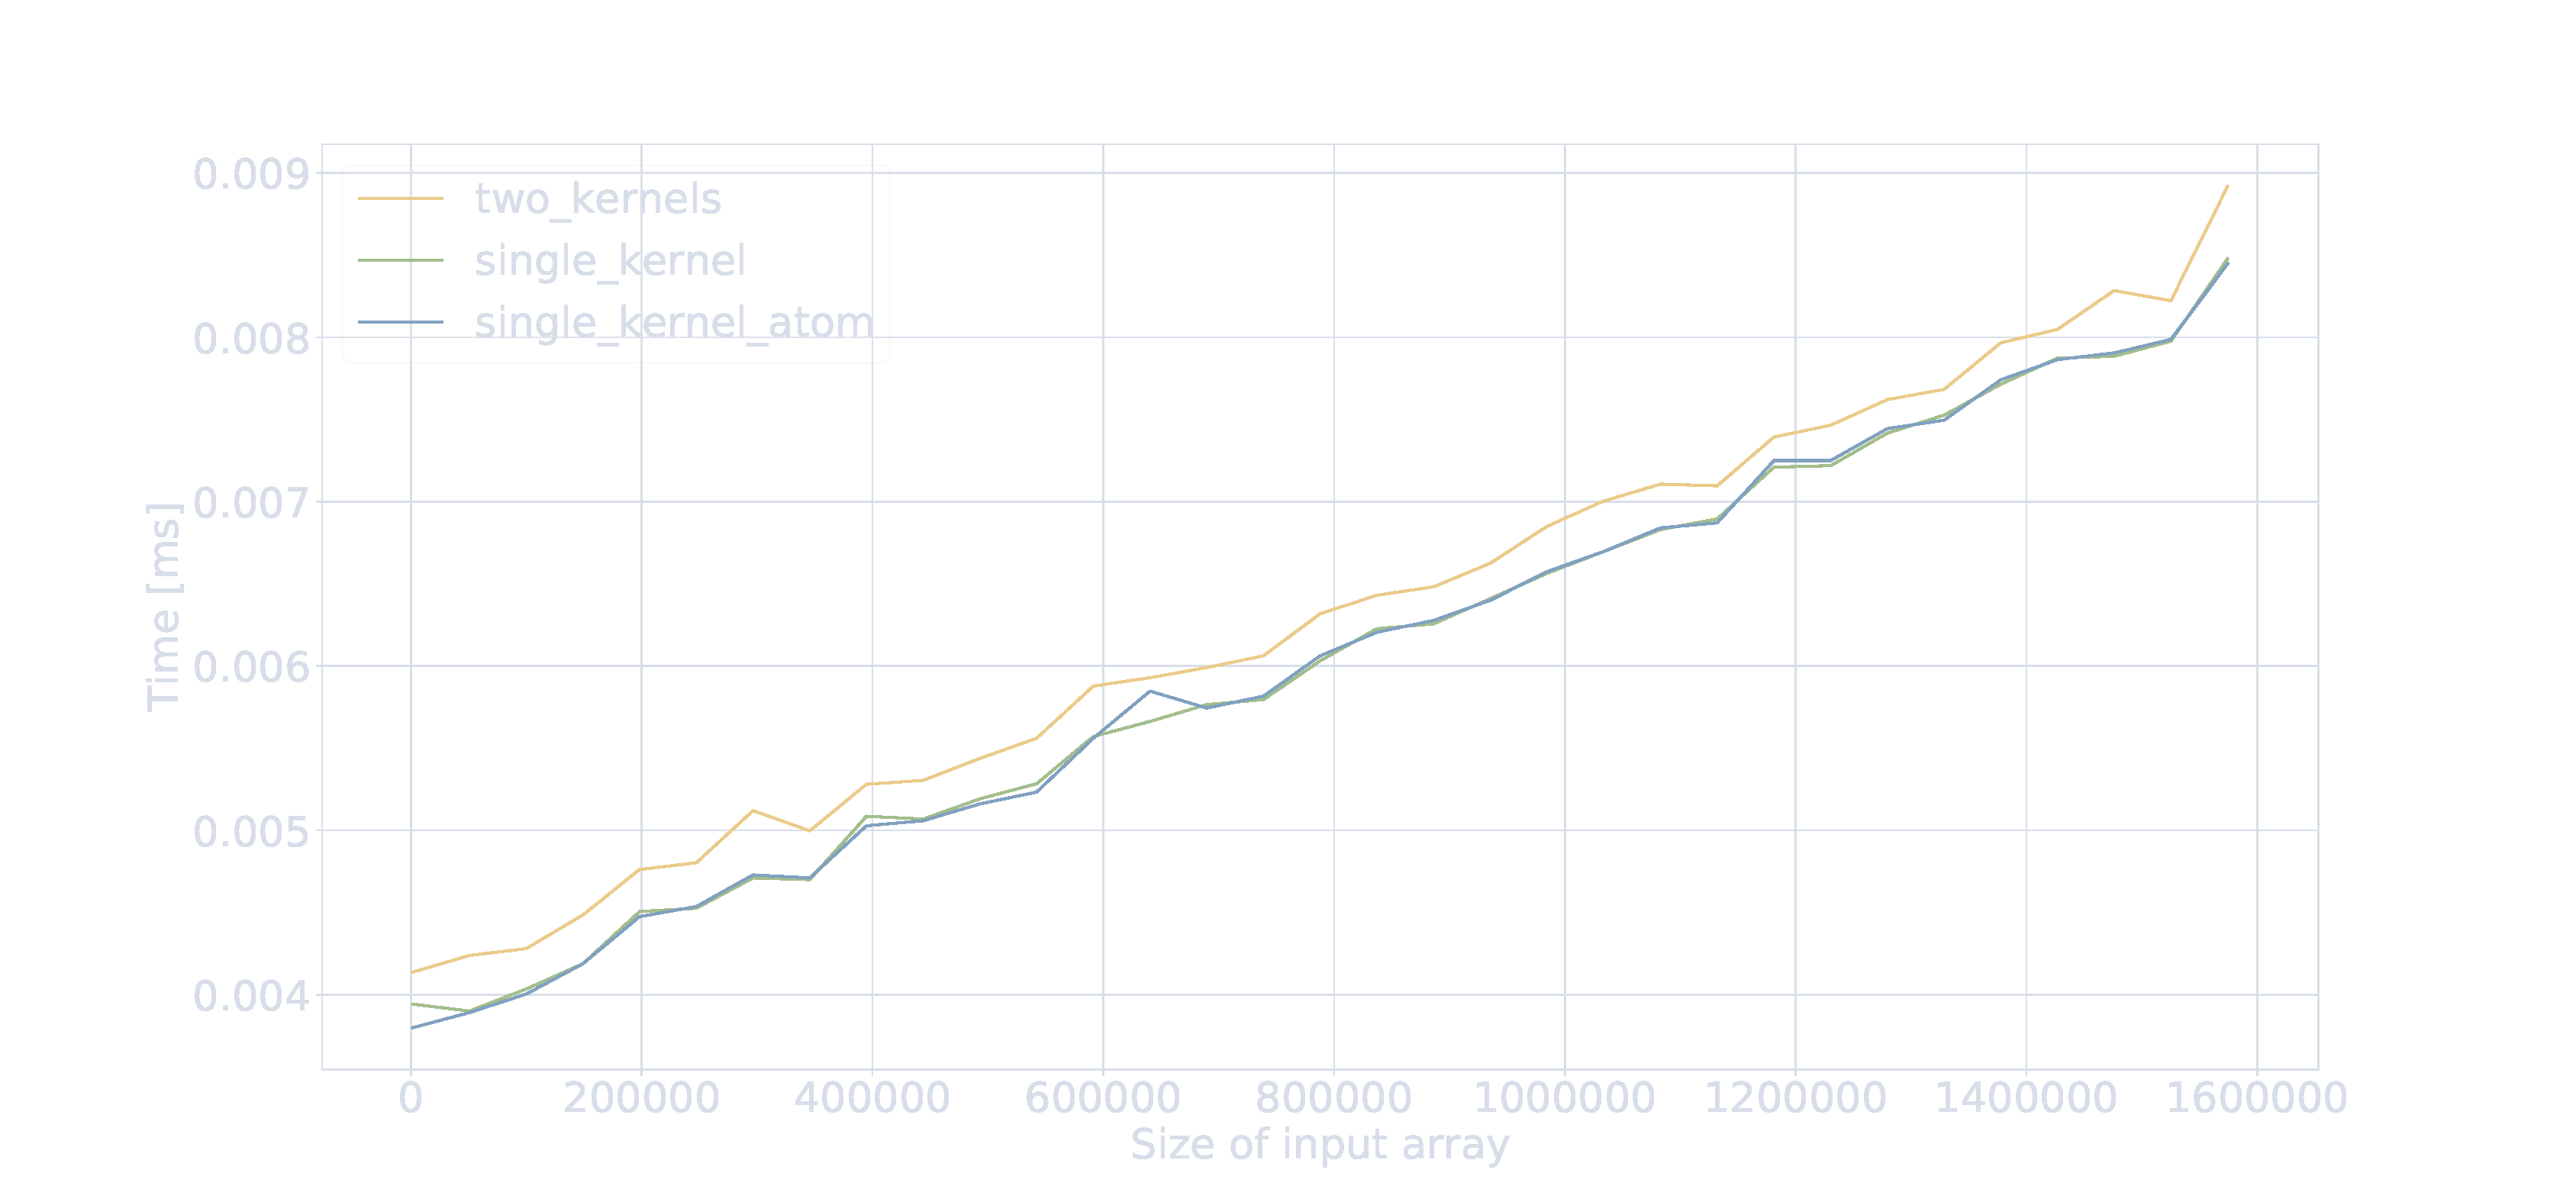
\includegraphics[width=0.9\textwidth]{reduce_atom.pdf}
	\end{figure}
\end{frame}

\begin{frame}[fragile]{Broadcast}{illustration}
	\centering
	\begin{figure}
		\centering
		\begin{tikzpicture}[square/.style={draw=black, thick, fill=NordBlue, text=NordDarkBlack,rectangle,minimum width=1cm,minimum height=1cm}]
		  \foreach \y in {1,...,5} {
				\foreach \x in {1,...,5} {
					\node[square] (n\x\y) at (\x cm,\y cm) {};
				}
			}
			\node[square] (n33t) at (3 cm,3 cm) {
\includegraphics[width=0.6cm]{thermometer.jpg}};
		\end{tikzpicture}
	\end{figure}
\end{frame}

\begin{frame}[fragile]{Broadcast}{illustration}
	\centering
	\begin{figure}
		\centering
		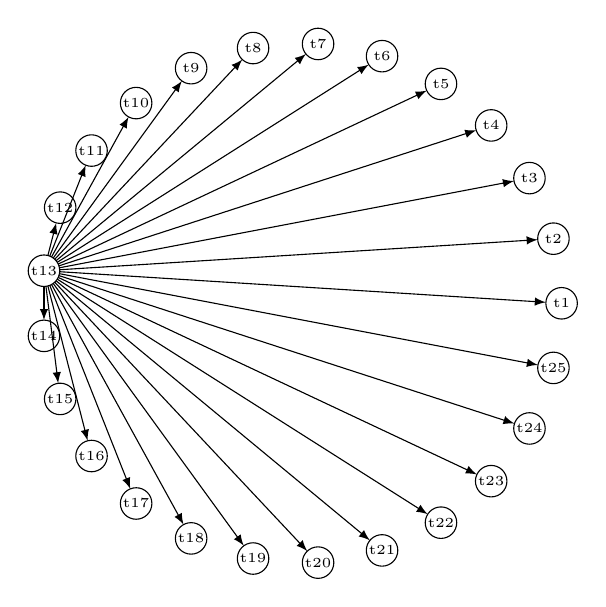
\begin{tikzpicture}
			\def \n {25}
			\def \radius {3.3cm}

			\foreach \s in {1,...,\n} {
				\node[draw, circle, minimum size=0.4cm, inner sep=0pt, outer sep=0pt] (n\s) at ({360/\n * (\s - 1)}:\radius) {\tiny t\s};
			}

			\foreach \s in {1,...,12} {
				\draw[->, >=latex] (n13) -- (n\s);
			}
			\foreach \s in {14,...,\n} {
				\draw[->, >=latex] (n13) -- (n\s);
			}
		\end{tikzpicture}
	\end{figure}
\end{frame}

\begin{frame}[fragile]{Broadcast}{basic version}
\centering
\begin{lstlisting}[showstringspaces=false]
unsigned int special_value = (unsigned int) -1;
unsigned int last_it = special_value;
int stride = blockDim.x * gridDim.x;


for (unsigned it = 0; it < last_it; it++) {
  int i = threadIdx.x + blockIdx.x * blockDim.x;
  for (; i < n; i += stride) {
    data[i] += value;
    if (data[i] > threshold)
      stop = true;
  }

  if (stop)
    last_it = it;
}
\end{lstlisting}
\end{frame}

\begin{frame}[fragile]{Broadcast}{volatile global}
	\begin{columns}
			\begin{column}{0.4\textwidth}
\begin{lstlisting}[title={sensor owner}]
if (data[i] > threshold)
  stop = true;

store (flag, stop, it + 1);
\end{lstlisting}
			\end{column}
			\begin{column}{0.4\textwidth}
\begin{lstlisting}[title={other threads}]
if (special_value == last_it) {
  status_word it_state 
    = load (flag);

  while (it_state.data <= it)
    it_state = load (flag);

  if (it_state.flag)
    last_it = it_state.data;
}
\end{lstlisting}
			\end{column}
	\end{columns}
\end{frame}

\begin{frame}[fragile]{Broadcast}{volatile global performance}
\centering
	\begin{figure}
		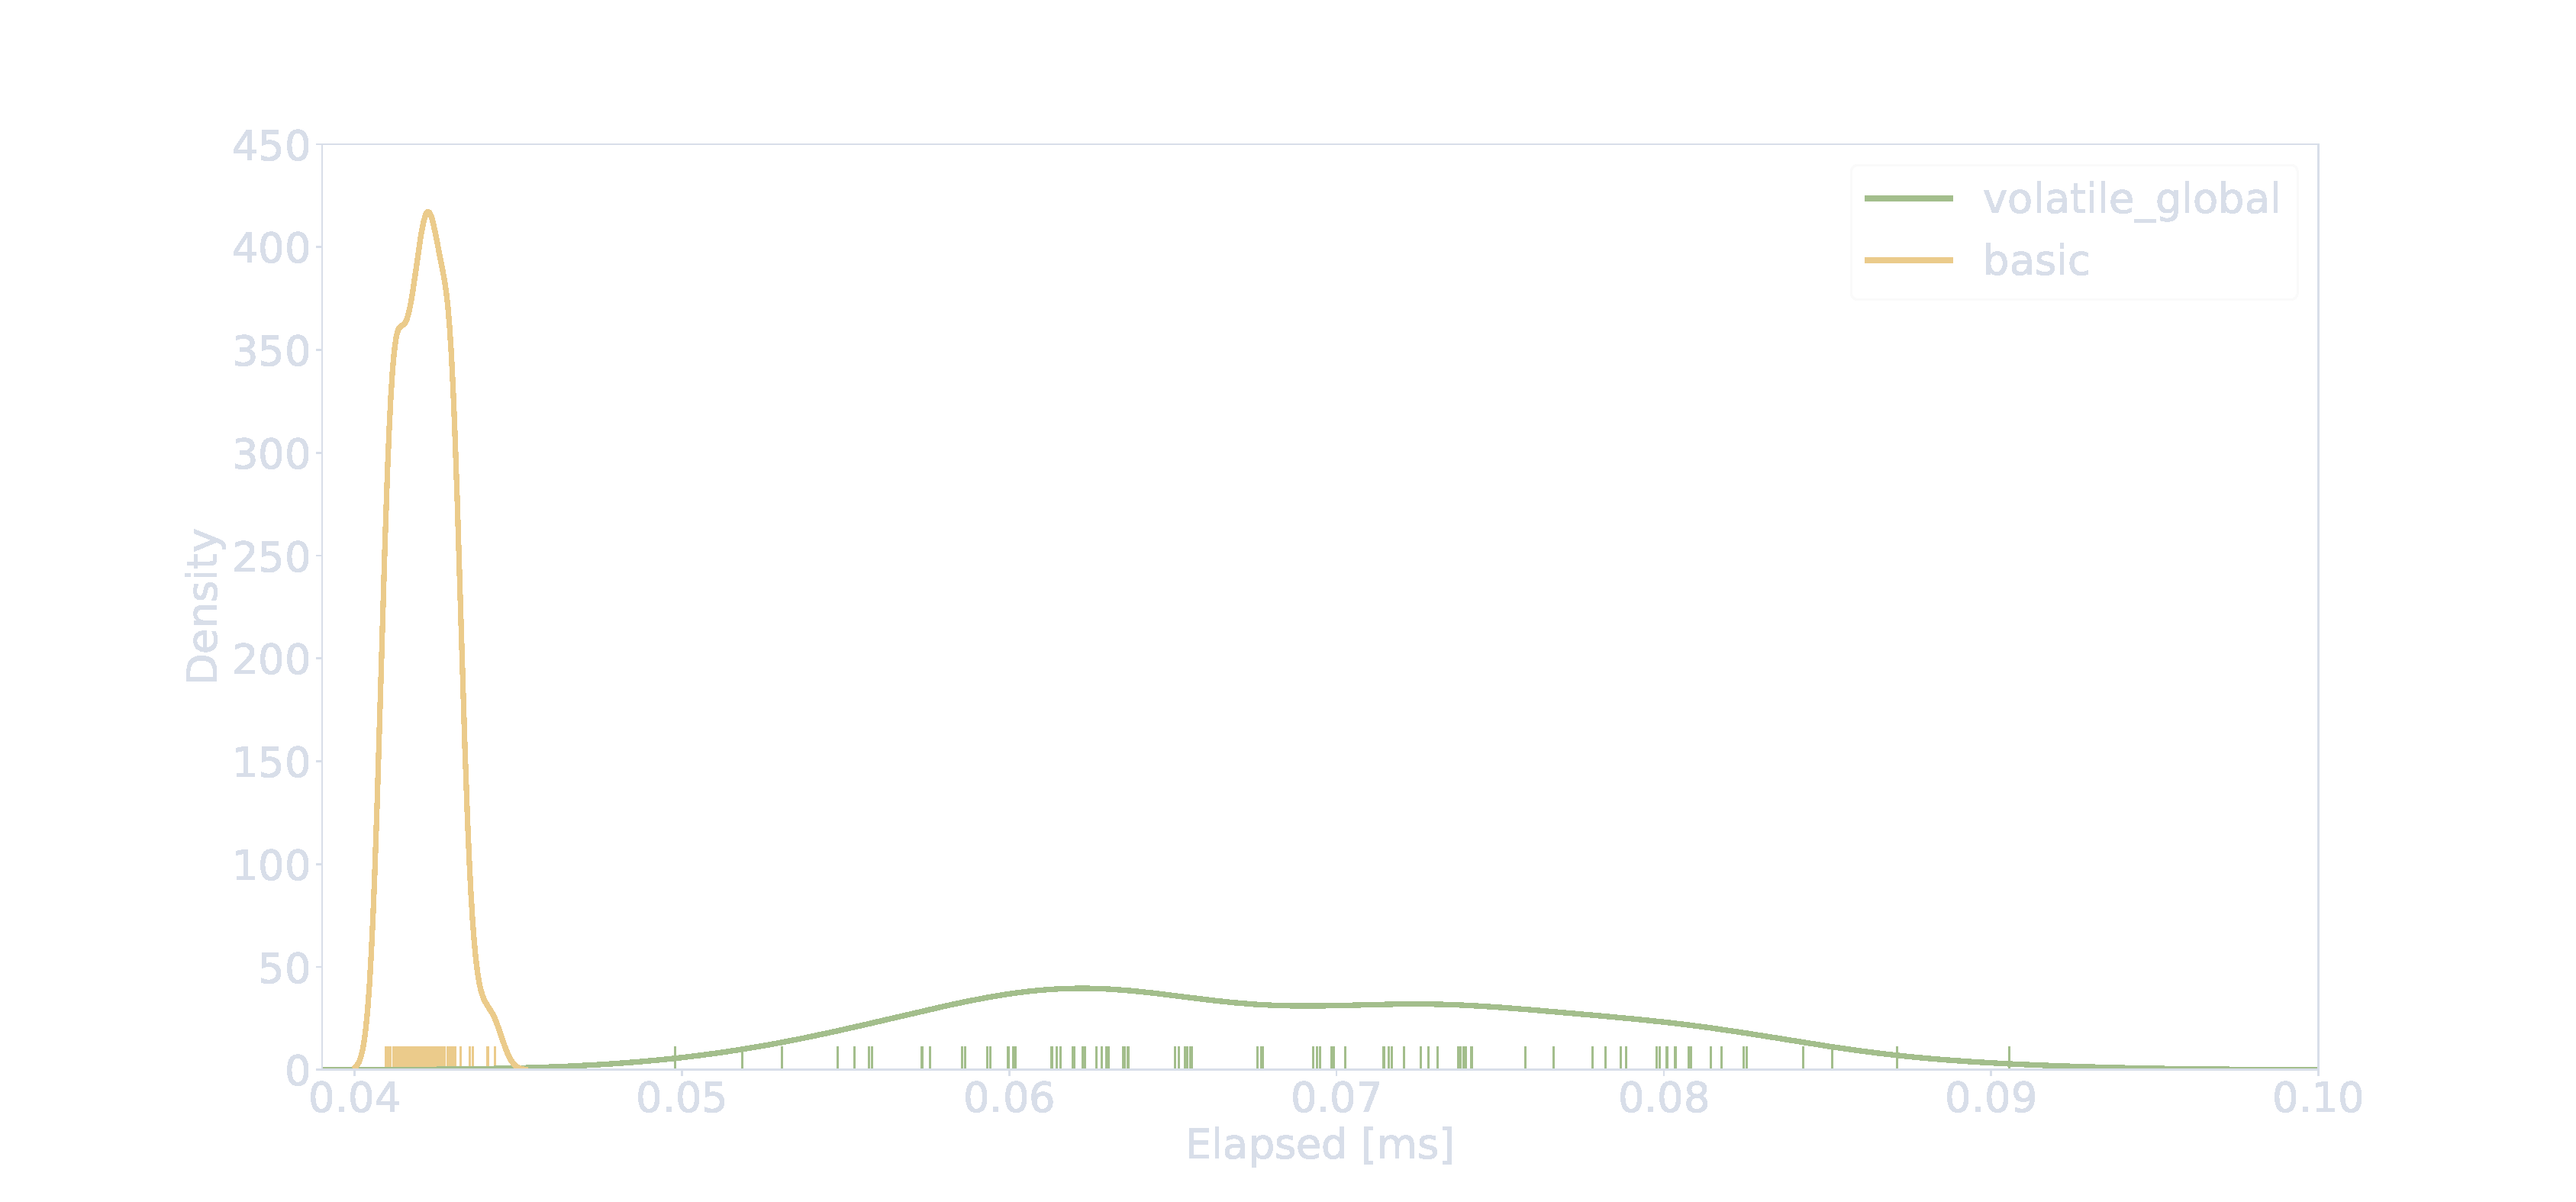
\includegraphics[width=0.9\textwidth]{density_02.pdf}
	\end{figure}
\end{frame}

\begin{frame}[fragile]{Broadcast}{volatile global block}
\centering
	\begin{columns}
			\begin{column}{0.6\textwidth}
\begin{lstlisting}[showstringspaces=false]
if (last_it == special_value) {
  if (threadIdx.x == 0) {
    status_word it_state = load (flag);

    while (it_state.data <= it)
      it_state = load (flag);

    if (it_state.flag)
      block_last_it = it_state.data;
  }
  __syncthreads ();

  last_it = block_last_it;
}
\end{lstlisting}
\end{column}
\end{columns}
\end{frame}

\begin{frame}[fragile]{Broadcast}{illustration}
	\centering
	\begin{figure}
		\centering
		\begin{tikzpicture}[square/.style={draw=black, thick, text=NordDarkBlack,rectangle,minimum width=1cm,minimum height=1cm}]
		  \foreach \y in {1,...,3} {
				\foreach \x in {1,...,5} {
					\node[fill=NordBlue, square] (n\x\y) at (\x cm,\y cm) {};
				}
			}
		  \foreach \y in {4,...,5} {
				\foreach \x in {1,...,5} {
					\node[fill=NordGreen, square] (n\x\y) at (\x cm,\y cm) {};
				}
			}
			\node[square] (n33t) at (3 cm,3 cm) {
\includegraphics[width=0.6cm]{thermometer.jpg}};
		\end{tikzpicture}
	\end{figure}
\end{frame}

\begin{frame}[fragile]{Broadcast}{illustration}
	\centering
	\begin{figure}
		\centering
		\begin{tikzpicture}
			\def \n {25}
			\def \radius {3.3cm}

			\foreach \s in {1,...,\n} {
				\node[draw, circle, minimum size=0.4cm, inner sep=0pt, outer sep=0pt] (n\s) at ({360/\n * (\s - 1)}:\radius) {\tiny t\s};
			}

			\foreach \s in {1,...,4} {
				\draw[->, >=latex] (n5) -- (n\s);
			}
			\foreach \s in {6,...,10} {
				\draw[->, >=latex] (n5) -- (n\s);
			}

			\foreach \s in {11,...,12} {
				\draw[->, >=latex] (n18) -- (n\s);
			}
			\foreach \s in {14,...,17} {
				\draw[->, >=latex] (n18) -- (n\s);
			}
			\foreach \s in {19,...,\n} {
				\draw[->, >=latex] (n18) -- (n\s);
			}

			\draw[NordGreen,->, >=latex,thick] (n13) -- (n5);
			\draw[NordBlue,->, >=latex,thick] (n13) -- (n18);
		\end{tikzpicture}
	\end{figure}
\end{frame}

\begin{frame}[fragile]{Broadcast}{volatile global block performance}
\centering
	\begin{figure}
		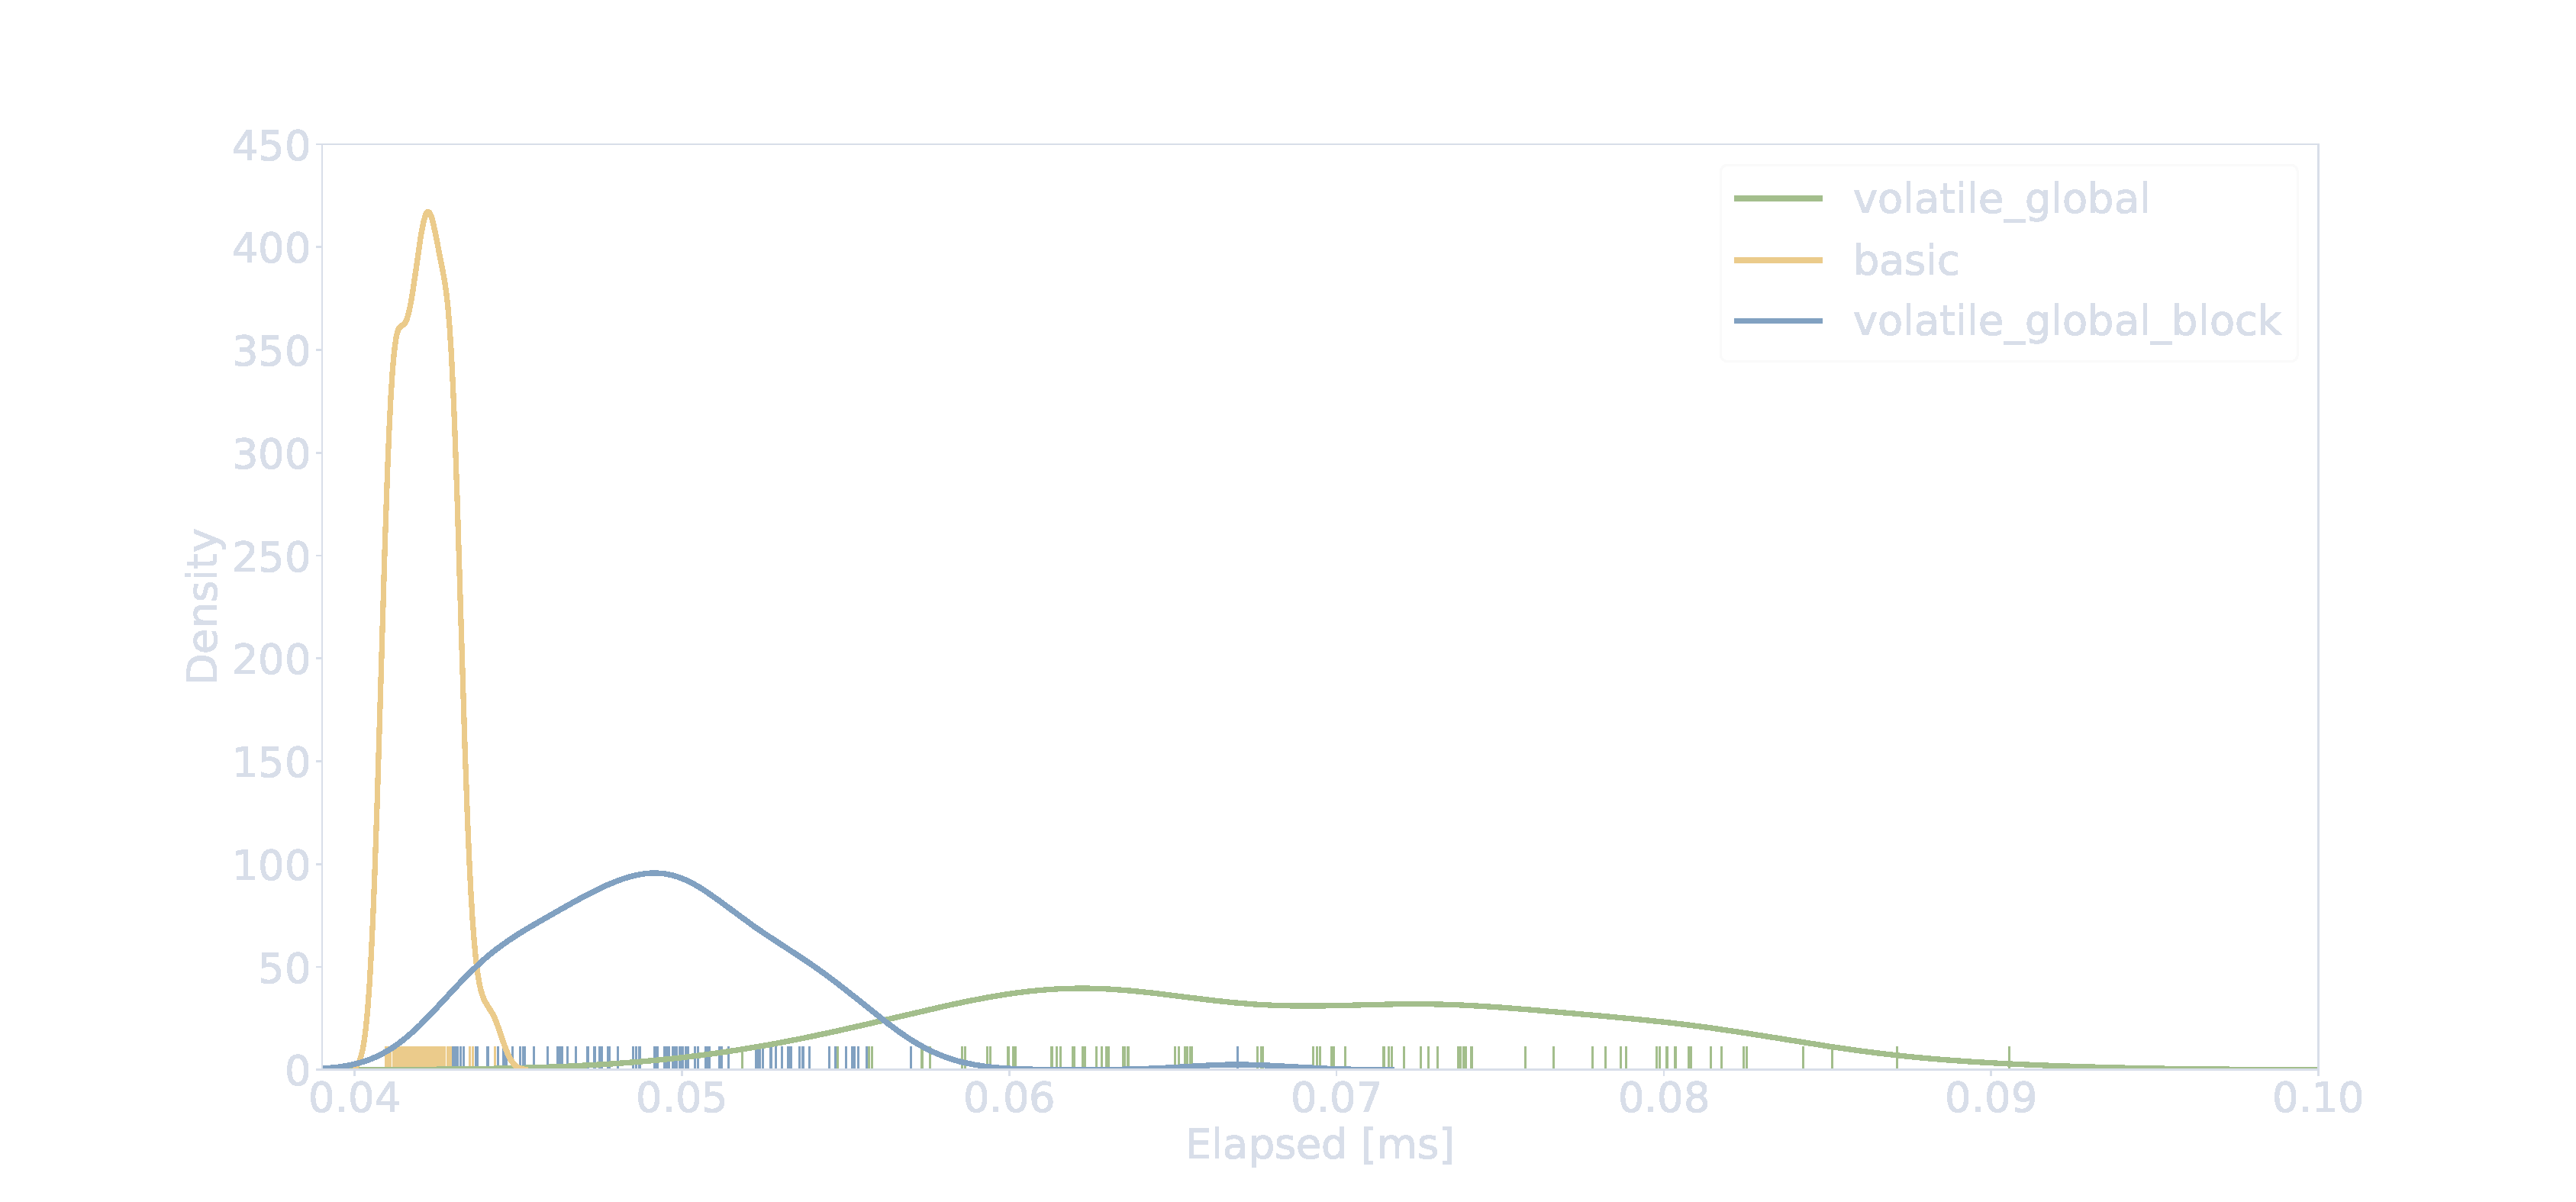
\includegraphics[width=0.9\textwidth]{density_03.pdf}
	\end{figure}
\end{frame}

\begin{frame}[fragile]{Broadcast}{volatile global block sleep}
\centering
	\begin{columns}
			\begin{column}{0.6\textwidth}
\begin{lstlisting}[showstringspaces=false]
if (last_it == special_value) {
  if (threadIdx.x == 0) {
    status_word it_state = load (flag);

    while (it_state.data <= it) {
      __nanosleep (250); //< new line 
      it_state = load (flag);
    }

    if (it_state.flag)
      block_last_it = it_state.data;
  }
  __syncthreads ();

  last_it = block_last_it;
}
\end{lstlisting}
\end{column}
\end{columns}
\end{frame}

\begin{frame}[fragile]{Broadcast}{volatile global block sleep performance}
\centering
	\begin{figure}
		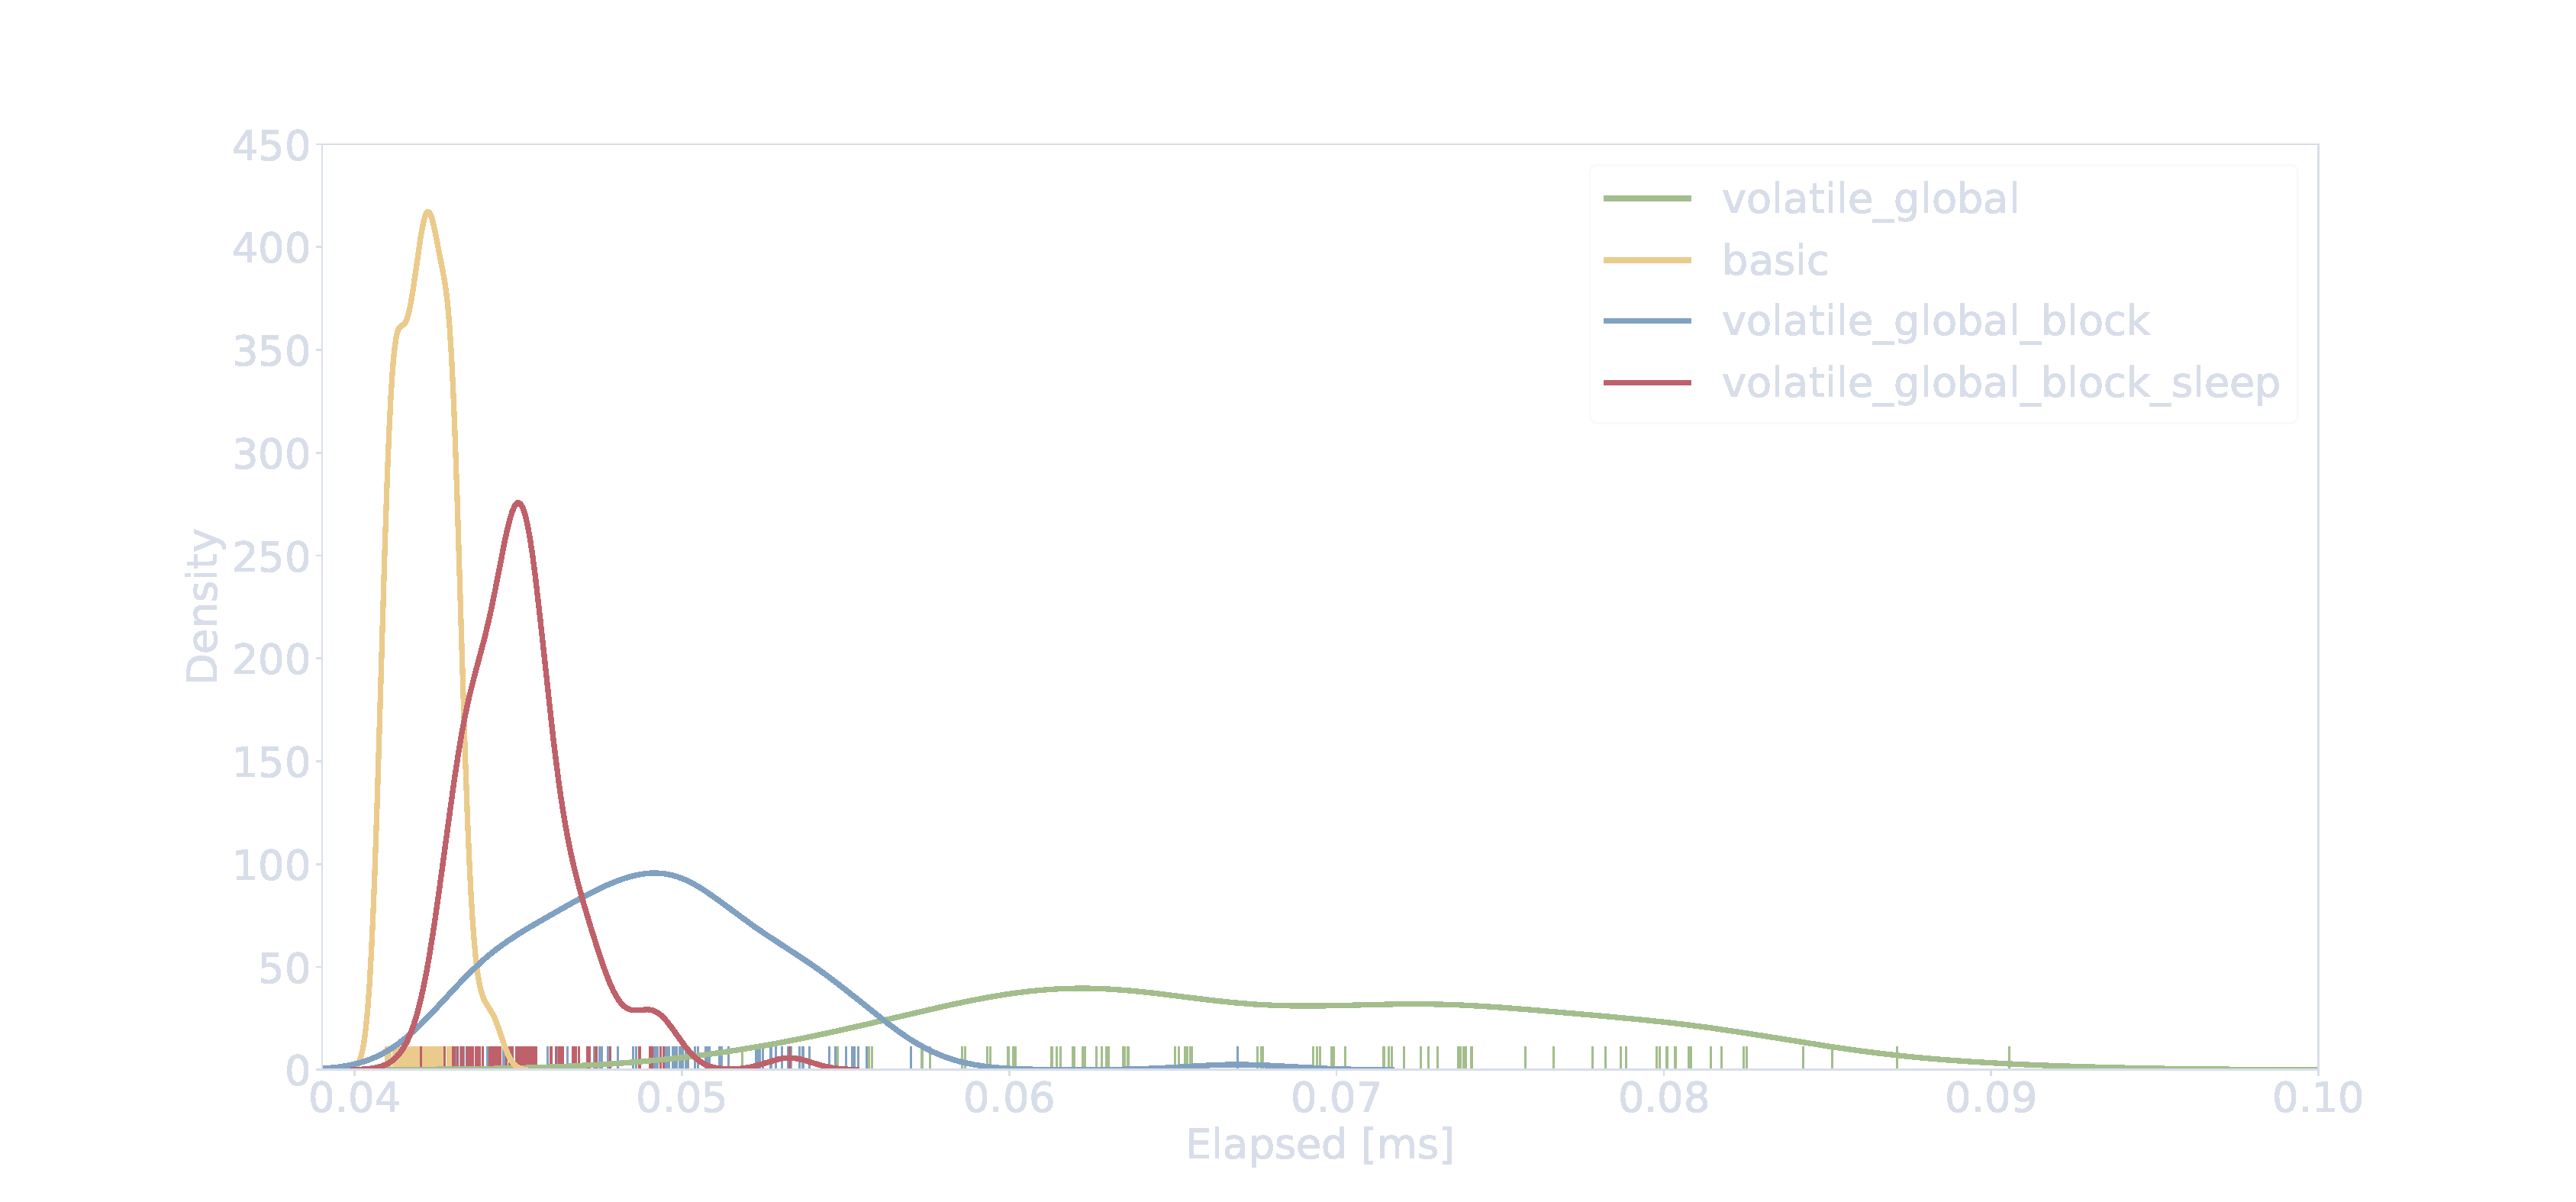
\includegraphics[width=0.9\textwidth]{density_04.pdf}
	\end{figure}
\end{frame}

\begin{frame}[fragile]{Broadcast}{atomic (sensor owner)}
	\begin{columns}
			\begin{column}{0.6\textwidth}
\begin{lstlisting}[]
if (data[i] > threshold)
  stop = true;

flag->store (
  status_word {stop, it + 1}, 
  cuda::memory_order_relaxed);
flag->notify_all ();
\end{lstlisting}
			\end{column}
	\end{columns}
\end{frame}

\begin{frame}[fragile]{Broadcast}{atomic}
	\begin{columns}
			\begin{column}{0.7\textwidth}
\begin{lstlisting}[title={other threads}]
if (threadIdx.x == 0) {
  status_word it_state 
    = flag->load (cuda::memory_order_relaxed);
  
  if (it_state.data <= it) {
    flag->wait (it_state, cuda::memory_order_relaxed);
    it_state = flag->load (cuda::memory_order_relaxed);
  }
  
  if (it_state.flag)
    block_last_it = it_state.data;
}
__syncthreads ();

last_it = block_last_it;
\end{lstlisting}
			\end{column}
	\end{columns}
\end{frame}

\begin{frame}[fragile]{Broadcast}{atomic performance}
\centering
	\begin{figure}
		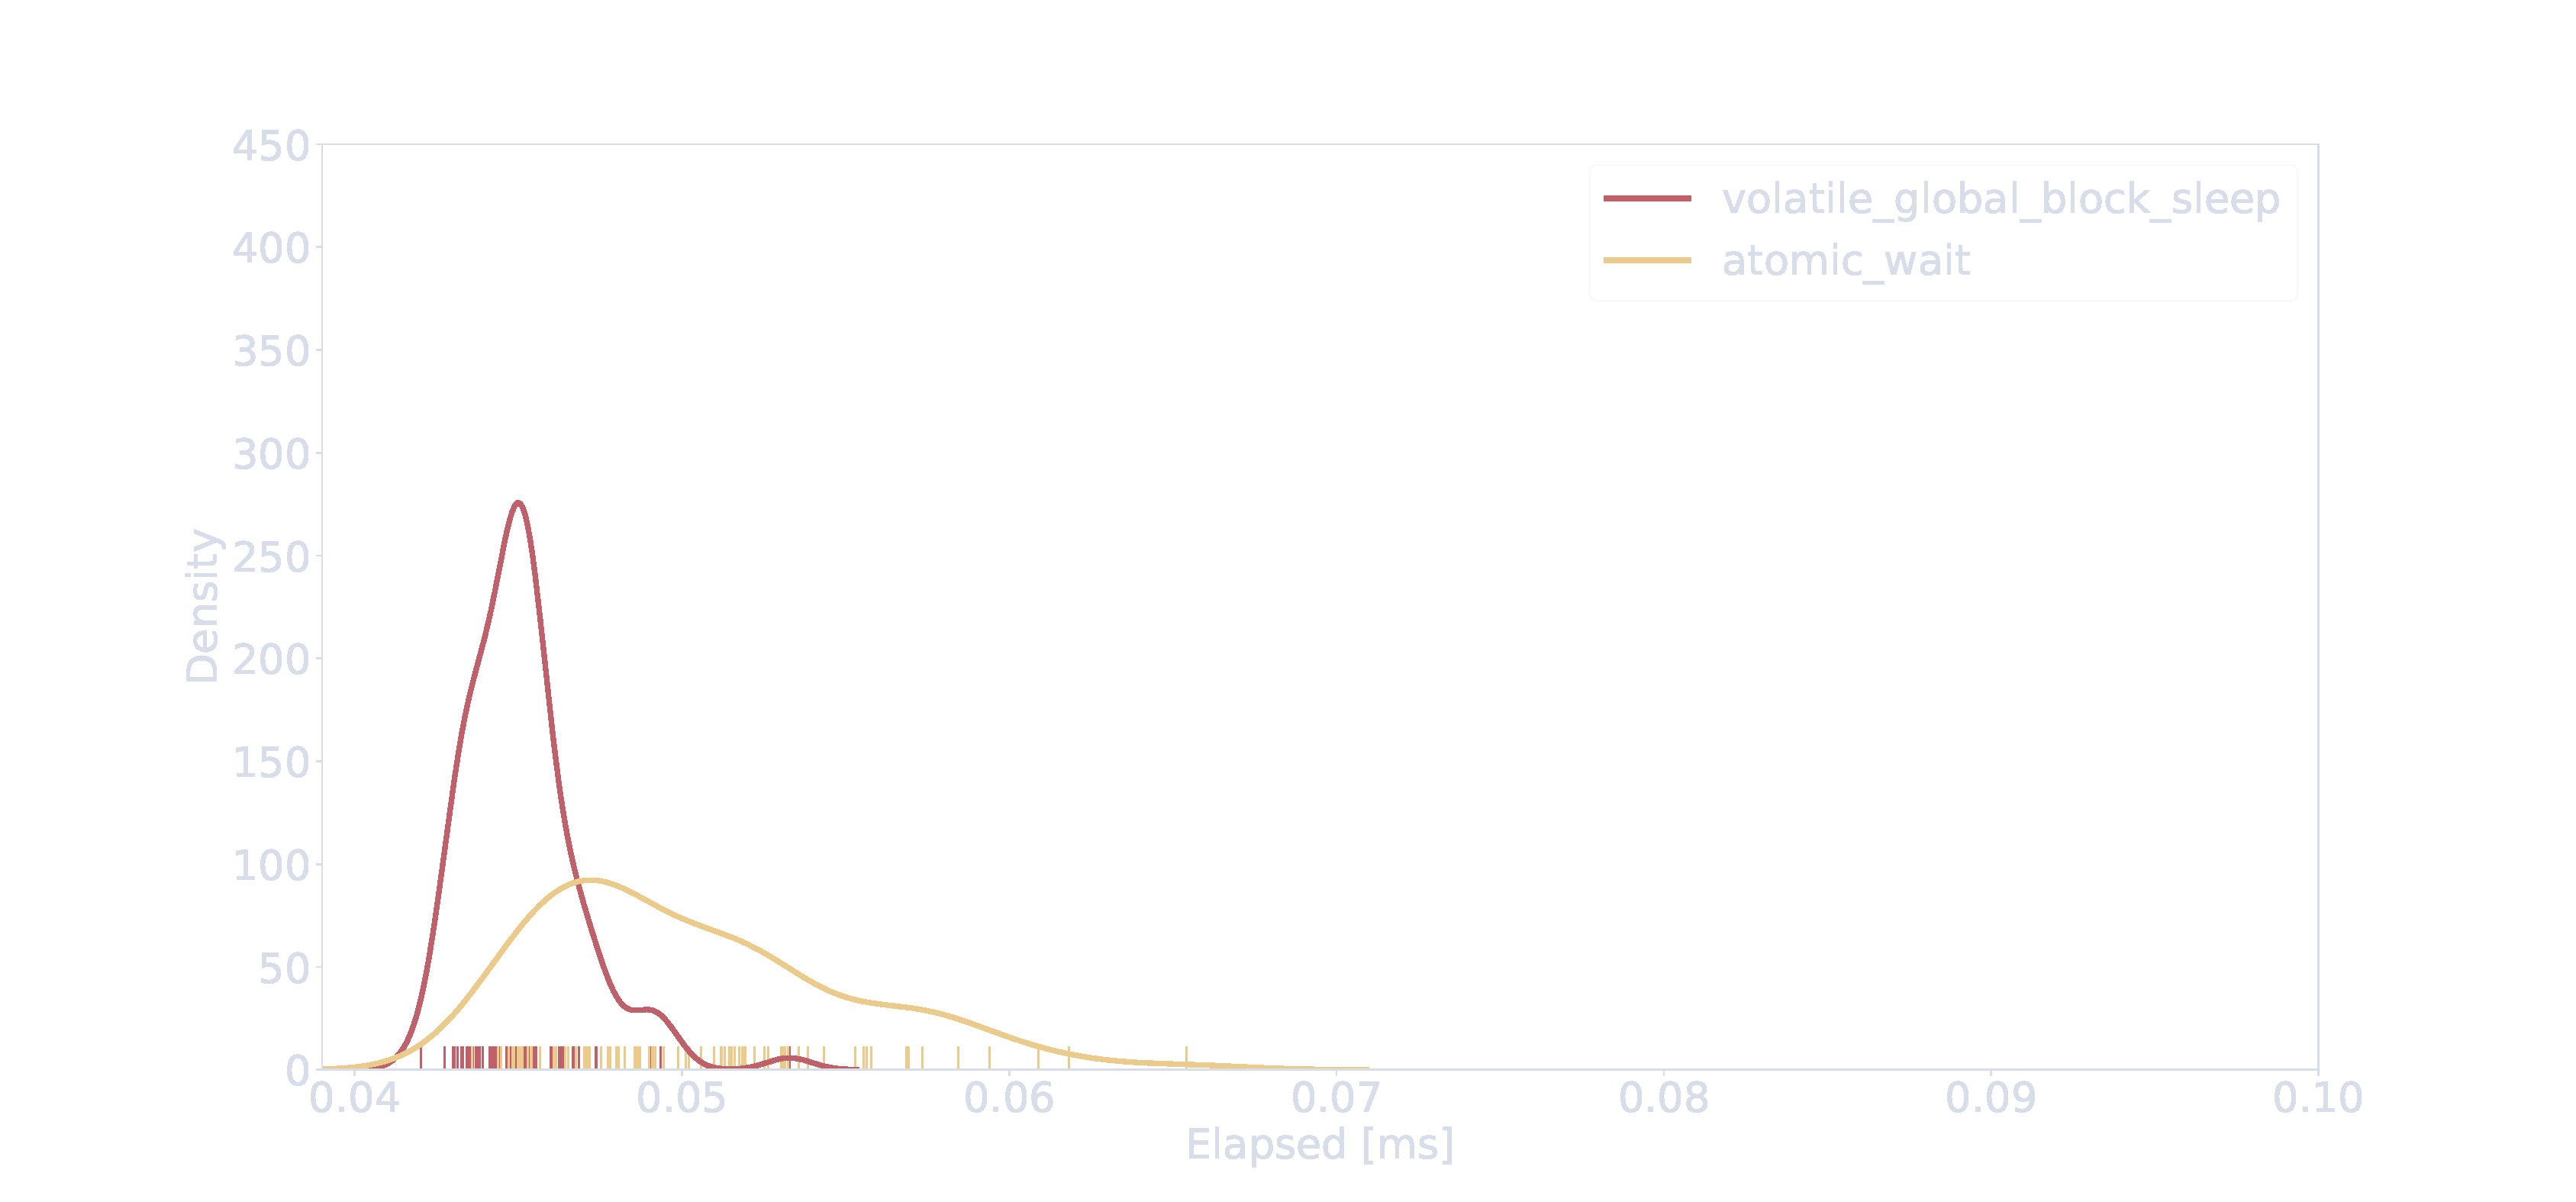
\includegraphics[width=0.9\textwidth]{density_atom_02.pdf}
	\end{figure}
\end{frame}

\begin{frame}[fragile]{Broadcast}{atomic performance}
\centering
	\begin{figure}
		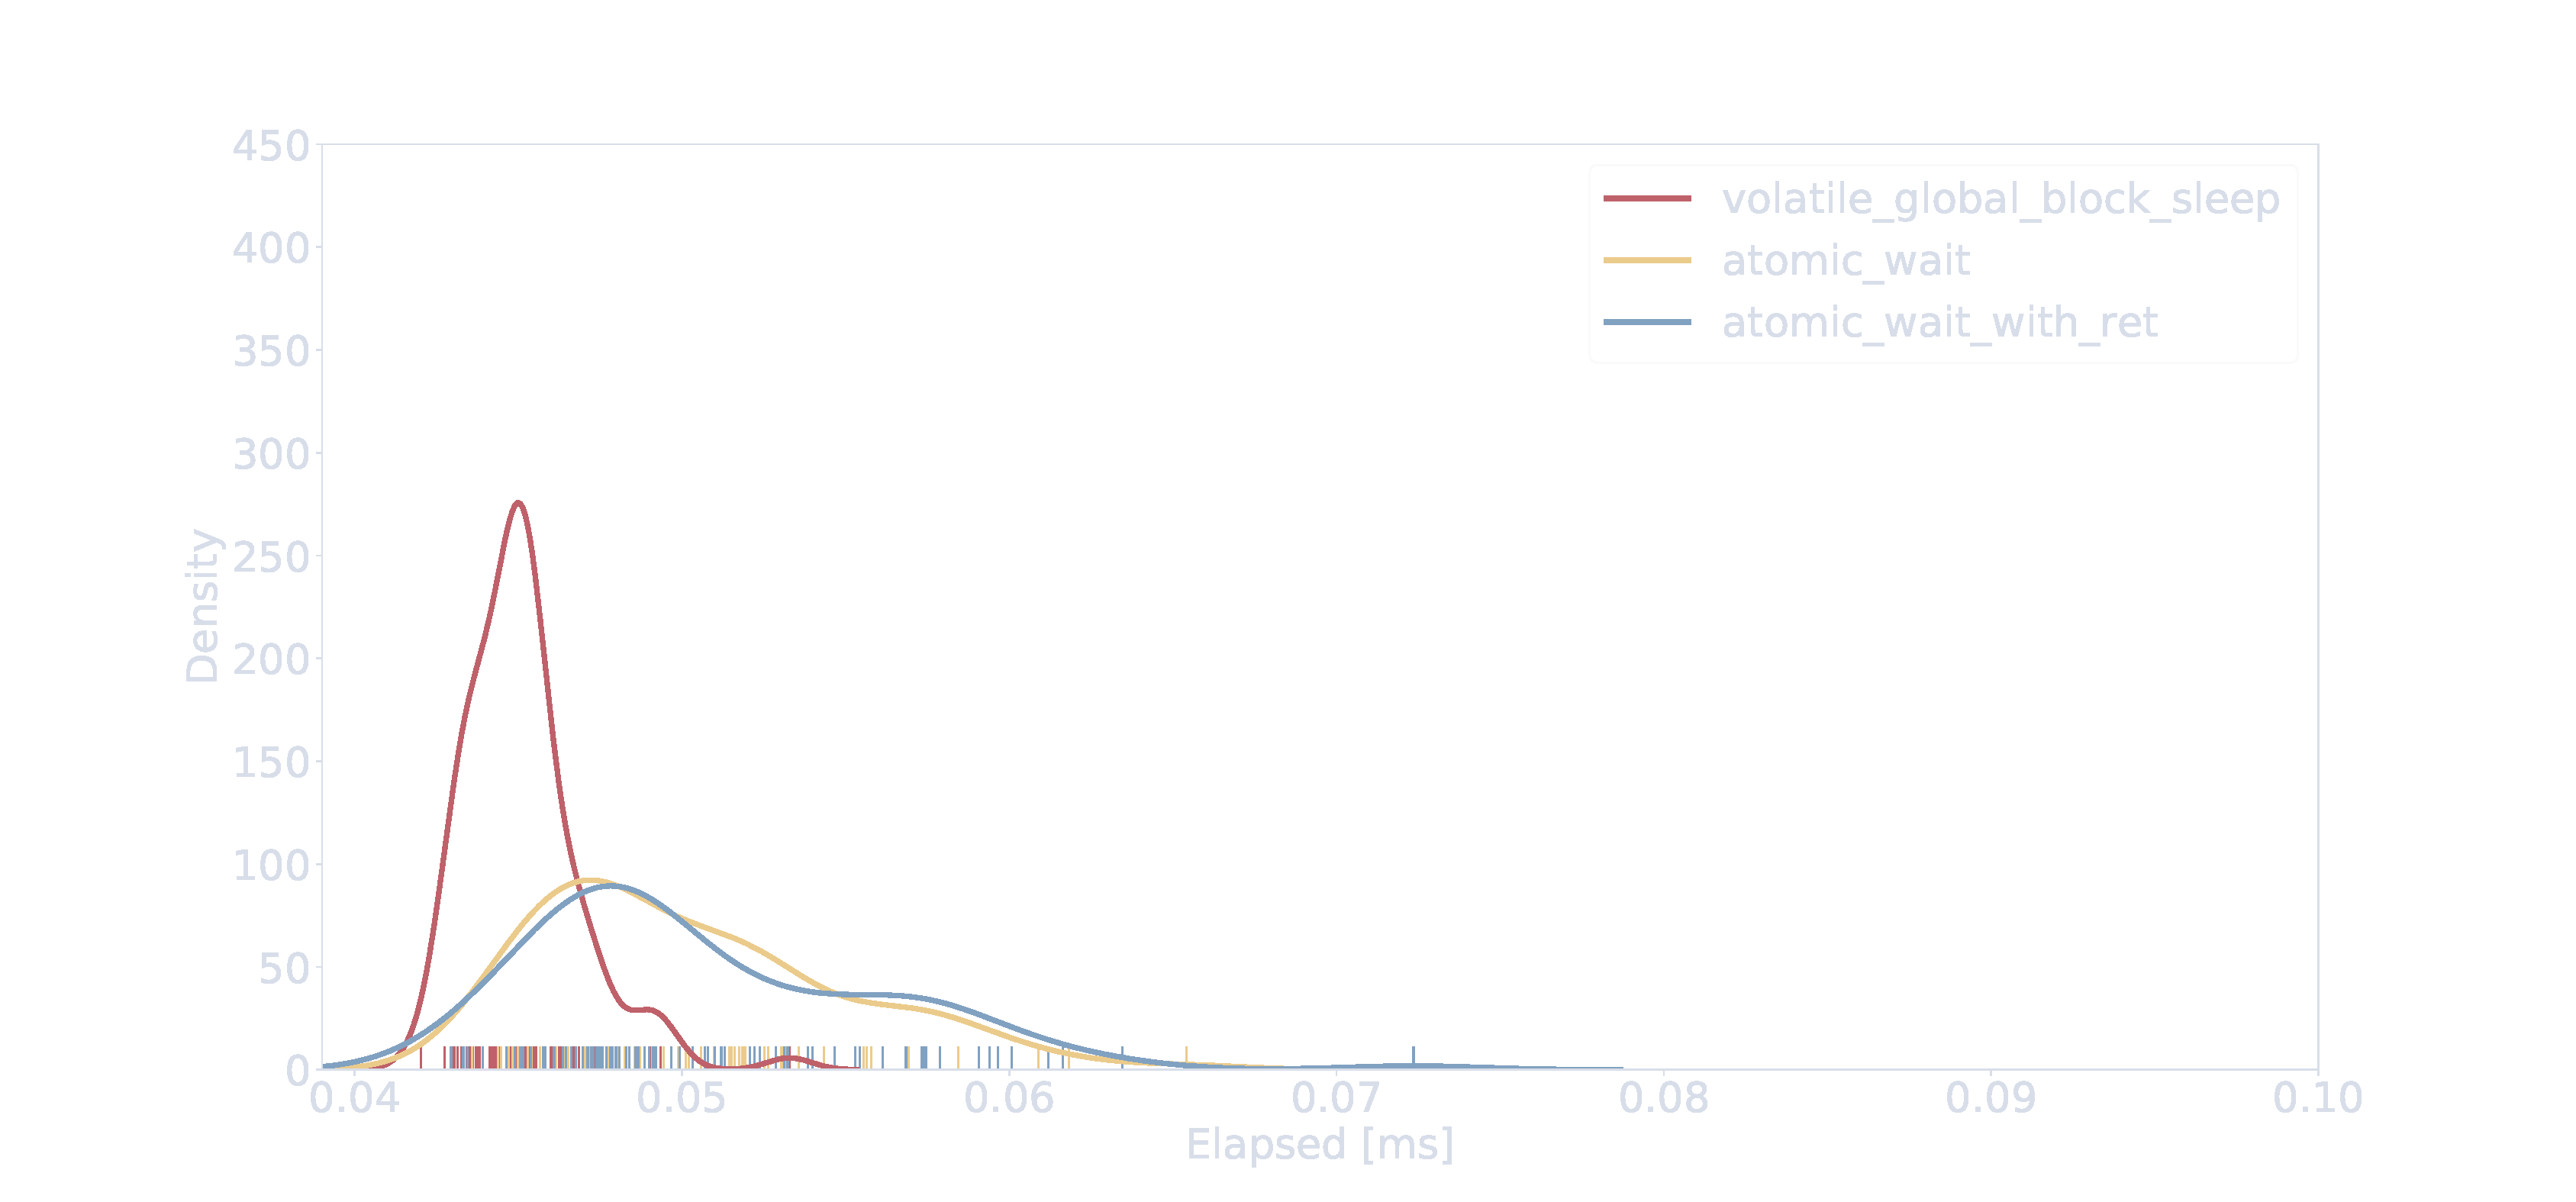
\includegraphics[width=0.9\textwidth]{density_atom_03.pdf}
	\end{figure}
\end{frame}

\begin{frame}[fragile]{Broadcast}{atomic performance}
\centering
	\begin{figure}
		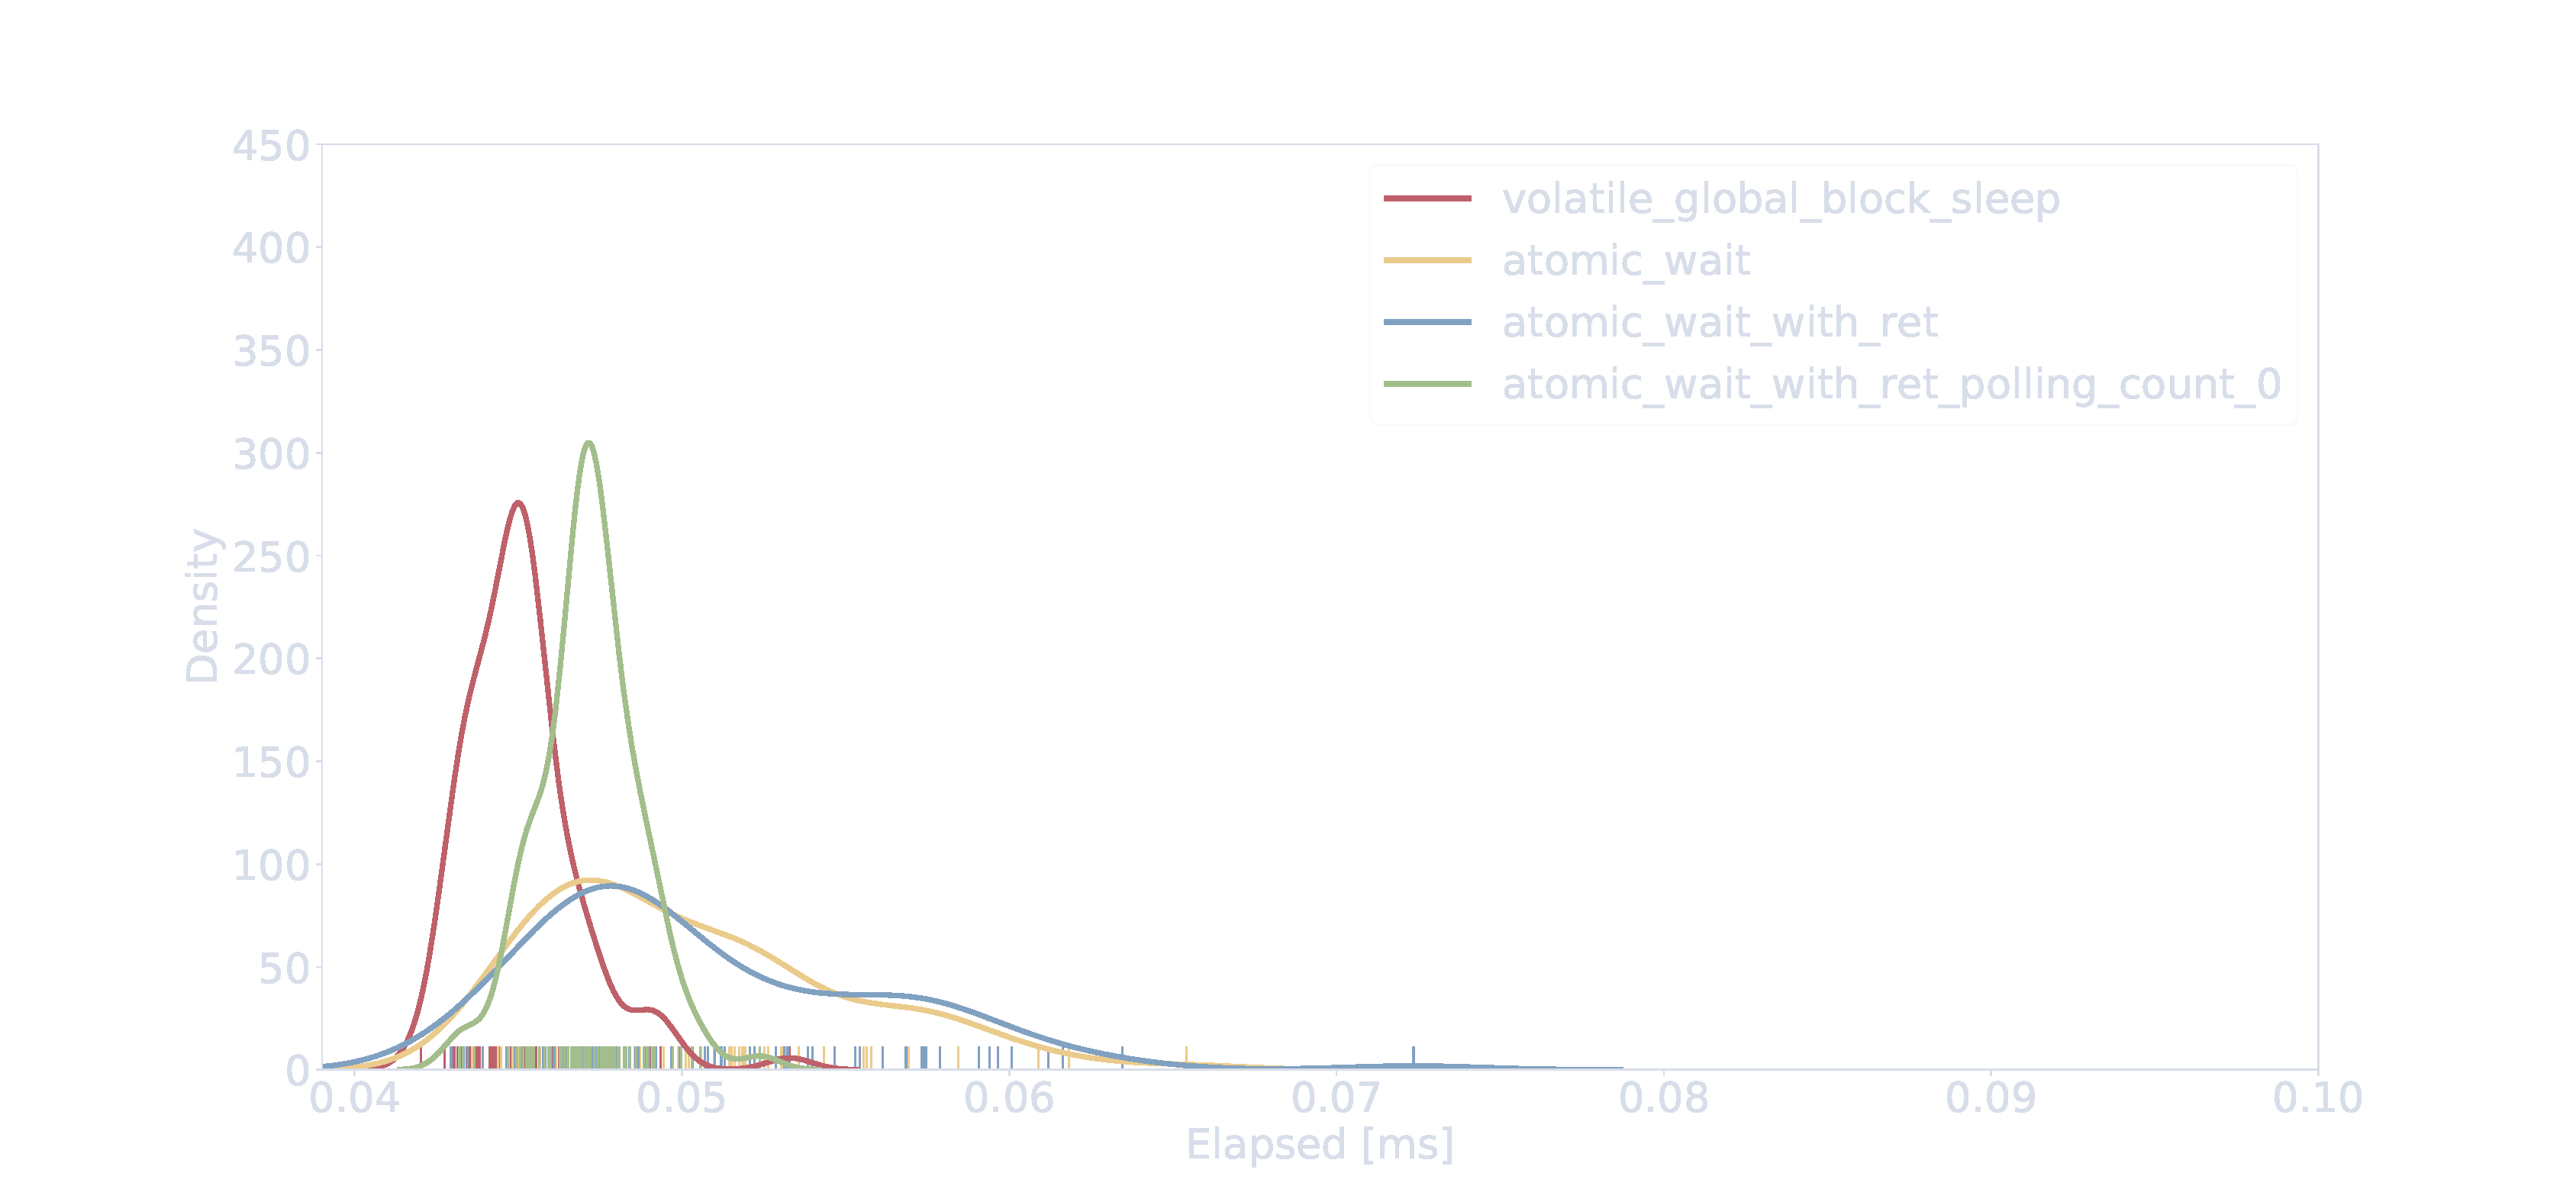
\includegraphics[width=0.9\textwidth]{density_atom_04.pdf}
	\end{figure}
\end{frame}

\begin{frame}[fragile]{Broadcast}{multi-GPU}
\centering
	\begin{figure}
		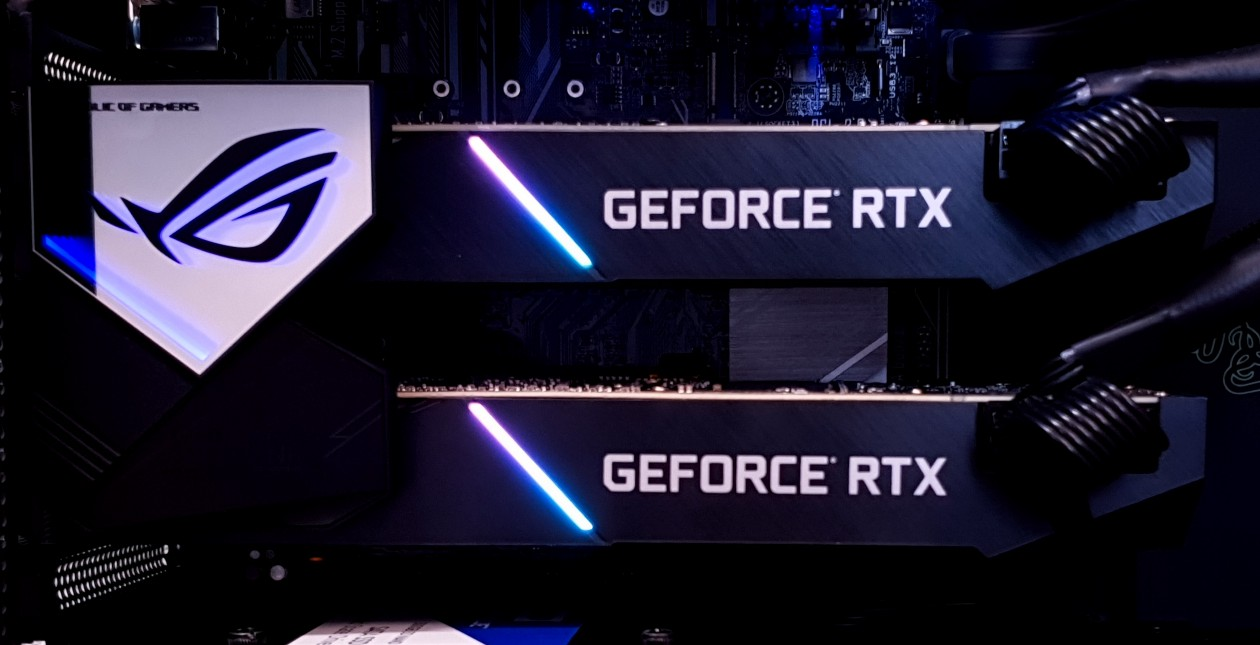
\includegraphics[width=0.7\textwidth]{nvlink.png}
	\end{figure}
\end{frame}

\begin{frame}[fragile]{Broadcast}{multi-GPU}
\centering
	\begin{figure}
		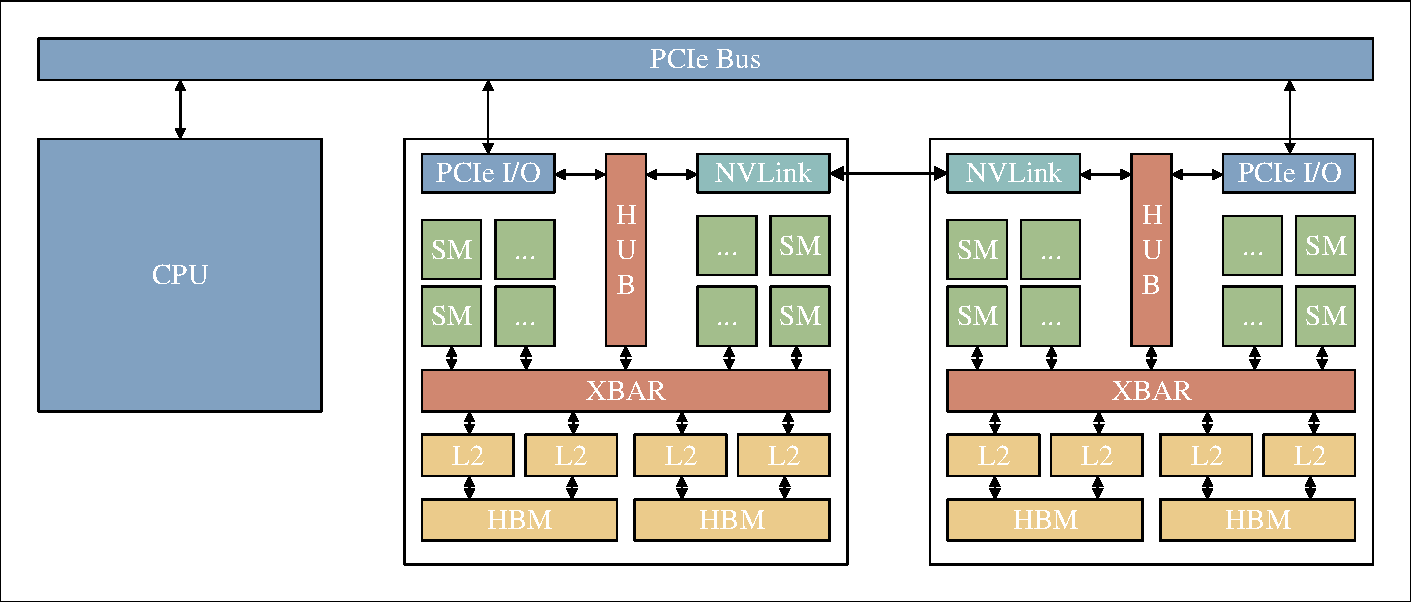
\includegraphics[trim=20 20 20 20,clip,width=\textwidth]{nvlink_architecture_mem_model.pdf}
	\end{figure}
\end{frame}

\begin{frame}[fragile]{Broadcast}{multi-GPU}
\centering
	\begin{figure}
		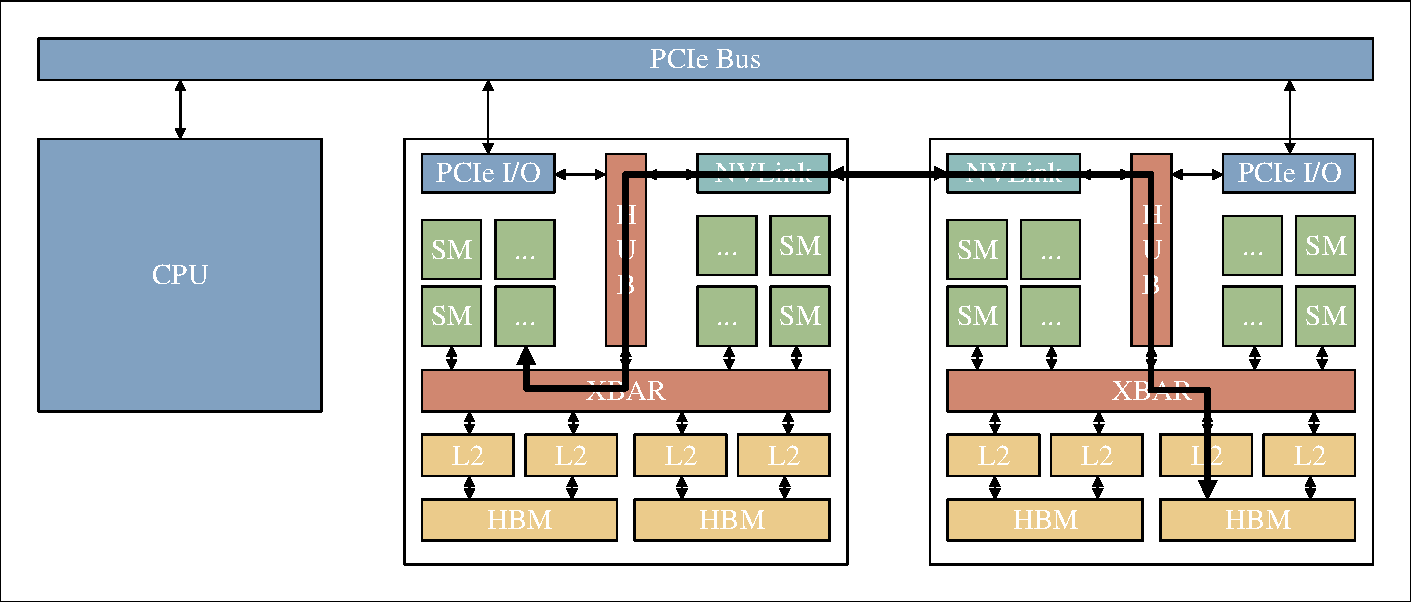
\includegraphics[trim=20 20 20 20,clip,width=\textwidth]{nvlink_architecture_mem_model_path.pdf}
	\end{figure}
\end{frame}

\begin{frame}[fragile]{Broadcast}{multi-GPU}
\centering
	\begin{figure}
		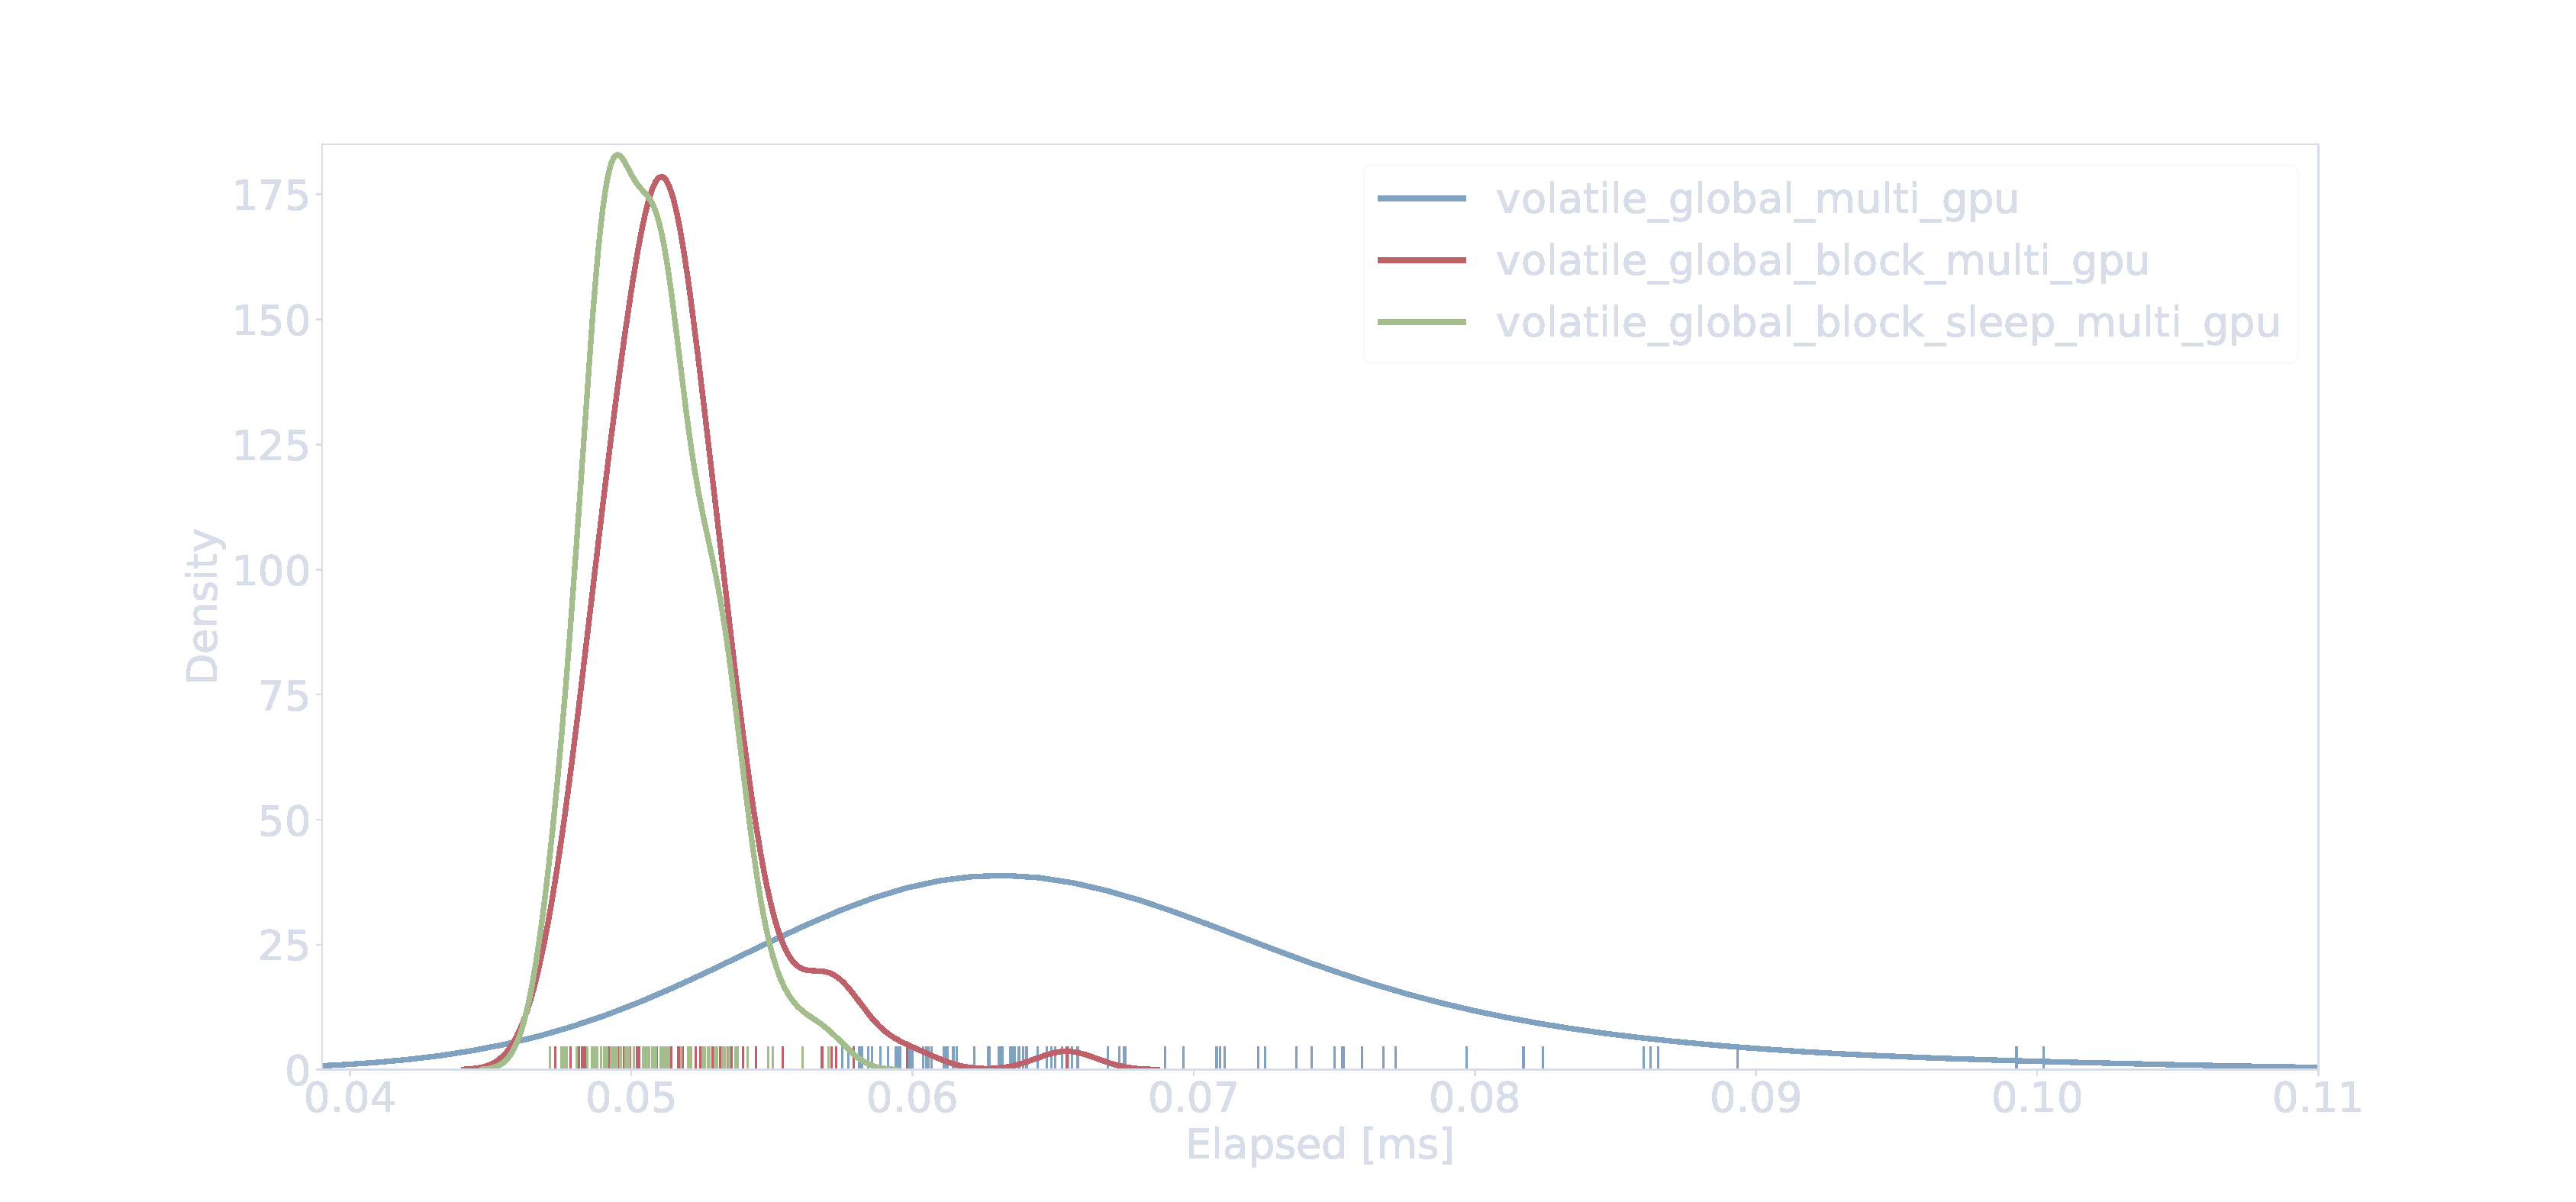
\includegraphics[width=\textwidth]{multi_gpu_density.pdf}
	\end{figure}
\end{frame}


\begin{frame}[fragile]{}{}
  Recommended materials
	\begin{itemize}
		\item CppCon 2018: Olivier Giroux ``High-Radix Concurrent C++.''
		\item CppCon 2019: Olivier Giroux ``The One-Decade Task: Putting std::atomic in CUDA.''
		\item Cpp Toronto 2020: Bryce Adelstein Lelbach ``The CUDA C++ Standard Library by.''
		\item Sorin, Daniel J. and Hill, Mark D. and Wood, David A. ``A Primer on Memory Consistency and Cache Coherence''
	\end{itemize}

  \vspace{0.1in}
	Source codes and presentation will be published soon, check \faTwitter @g\_evtushenko
\end{frame}

\end{document}

%%% Local Variables:
%%% mode: latex
%%% TeX-master: t
%%% TeX-engine: xetex
%%% End:
